% =========================================================================
% PROBLEMAS DE FLUXOS EM REDES — LIVRO / MONOGRAFIA INDEPENDENTE
% =========================================================================
\documentclass[11pt,a4paper,oneside]{book}

\usepackage{geometry}
\geometry{
    a4paper,
    left=2.4cm,
    right=2.4cm,
    top=2.7cm,
    bottom=2.7cm,
    headheight=14.5pt
}

\RequirePackage{fix-cm}
% =========================================================================
% CABEÇALHO UNIFICADO E DESIGN SYSTEM (NETWORKS FLOW)
% =========================================================================

% =========================================================================
% PACOTES FUNDAMENTAIS
% =========================================================================
\usepackage{amssymb}
\usepackage{amsmath}
\usepackage{amsthm}
\usepackage{bm}
\usepackage{enumitem}
\usepackage{mathtools}
\usepackage{lipsum}
\usepackage[brazilian]{babel}
\usepackage[utf8]{inputenc}
\usepackage[T1]{fontenc}
\usepackage[pdftex]{graphicx}
\usepackage{color}
\usepackage{xcolor}
\usepackage{colortbl}
\usepackage{tikz}
\usetikzlibrary{arrows.meta, calc, positioning, decorations.markings}
\usepackage{verbatim}
\usepackage[hyphens]{url}
\usepackage{longtable}
\usepackage{booktabs}
\usepackage[section]{placeins}
\usepackage{listings}
\usepackage{anyfontsize}
\usepackage{lmodern}
\usepackage{helvet}
\renewcommand{\familydefault}{\sfdefault}
\usepackage{fancyhdr}

\newif\ifapendiceteorico
\apendiceteoricofalse
\newif\ifapendicecodigo
\apendicecodigotrue

\fancypagestyle{textual}{%
    \fancyhf{}%
    \fancyhead[L]{\small\textsf{\nouppercase{\leftmark}}}%
    \fancyhead[R]{\small\textsf{\textbf{\thepage}}}%
    \fancyfoot{}%
    \renewcommand{\headrulewidth}{0.4pt}%
    \renewcommand{\footrulewidth}{0pt}%
}

\fancypagestyle{plain}{%
    \fancyhf{}%
    \fancyhead[R]{\small\textsf{\textbf{\thepage}}}%
    \fancyfoot{}%
    \renewcommand{\headrulewidth}{0pt}%
    \renewcommand{\footrulewidth}{0pt}%
}

\usepackage{titlesec}
\usepackage{setspace}
\usepackage[plainpages=false,pdfpagelabels]{hyperref}

\hypersetup{
    colorlinks=true,
    linkcolor=blue!80!black,
    citecolor=green!50!black,
    urlcolor=blue!60!black
}

% =========================================================================
% LISTAGENS DE CÓDIGO-FONTE C++ (LISTINGS)
% =========================================================================

% -------------------------------------------------------------------------
% Paleta de Cores de Sintaxe
% -------------------------------------------------------------------------
\definecolor{codegreen}{rgb}{0,0.6,0}
\definecolor{codegray}{rgb}{0.5,0.5,0.5}
\definecolor{codepurple}{rgb}{0.58,0,0.82}
\definecolor{backcolour}{rgb}{0.9,0.9,0.9}

% -------------------------------------------------------------------------
% Configurações Globais do Listings
% -------------------------------------------------------------------------
\lstset{
    language=C++,
    basicstyle=\ttfamily\small,
    tabsize=4,
    keepspaces=true,
    columns=fullflexible,
    lineskip=-2pt,
    backgroundcolor=\color{backcolour},
    commentstyle=\color{codegreen},
    keywordstyle=\color{blue}\bfseries,
    stringstyle=\color{codepurple},
    deletestring={[b]'},
    numbers=left,
    numberstyle=\tiny\color{codegray},
    numbersep=6pt,
    breaklines=true,
    breakatwhitespace=false,
    showspaces=false,
    showstringspaces=false,
    showtabs=false,
    frame=single,
    rulecolor=\color{black},
    captionpos=b
}

% =========================================================================
% ESTRUTURAS SEMÂNTICAS, TEOREMAS E DEFINIÇÕES
% =========================================================================
\newtheorem{prop}{Proposição}

% -------------------------------------------------------------------------
% Definições Formais
% -------------------------------------------------------------------------
\newcounter{definicao}
\renewcommand{\thedefinicao}{\arabic{definicao}}
\NewDocumentEnvironment{definicao}{o o}{%
    \par\addvspace{0.8\baselineskip}\noindent
    \refstepcounter{definicao}%
    \IfValueT{#2}{\label{#2}}%
    \textbf{Definição~\thedefinicao\IfValueT{#1}{ (#1)}}.%
    \space
}{%
    \par\addvspace{0.5\baselineskip}
}

% -------------------------------------------------------------------------
% Teoremas e Demonstrações
% -------------------------------------------------------------------------
\newcounter{teorema}
\renewcommand{\theteorema}{\arabic{teorema}}
\NewDocumentEnvironment{teorema}{o o}{%
    \par\addvspace{0.8\baselineskip}\noindent
    \refstepcounter{teorema}%
    \IfValueT{#2}{\label{#2}}%
    \textbf{Teorema~\theteorema\IfValueT{#1}{ (#1)}}.%
    \space\itshape
}{%
    \par\addvspace{0.5\baselineskip}
}

\NewDocumentEnvironment{demonstracao}{}{%
    \par\noindent\textbf{Demonstração.}\space
}{%
    \hfill $\blacksquare$\par\addvspace{0.5\baselineskip}
}

% -------------------------------------------------------------------------
% Macros Conceituais e Auxiliares
% -------------------------------------------------------------------------
\newcommand{\intuicao}[1]{\paragraph{Intuição #1.}}
\newcommand{\implicacoes}[1]{\paragraph{Implicações Estratégicas #1.}}
\newcommand{\sa}{\text{s.a.}\quad}

% =========================================================================
% PALETA CROMÁTICA SEMÂNTICA (DESIGN SYSTEM)
% =========================================================================

% -------------------------------------------------------------------------
% Partições S e T
% -------------------------------------------------------------------------
\definecolor{setSborder}{RGB}{22, 101, 52}
\definecolor{setStext}{RGB}{20, 83, 45}
\definecolor{setSsource}{RGB}{187, 247, 208}
\definecolor{setSnode}{RGB}{220, 252, 231}
\colorlet{setSbg}{green!10}

\definecolor{setTborder}{RGB}{190, 18, 60}
\definecolor{setTtext}{RGB}{159, 18, 57}
\definecolor{setTsink}{RGB}{254, 205, 211}
\definecolor{setTnode}{RGB}{255, 228, 230}
\colorlet{setTbg}{red!10}

% -------------------------------------------------------------------------
% Fronteira de Corte e Elementos Neutros
% -------------------------------------------------------------------------
\definecolor{cutviolet}{RGB}{109, 40, 217}
\definecolor{cutred}{RGB}{225, 29, 72}
\definecolor{darkslate}{RGB}{30, 41, 59}

% -------------------------------------------------------------------------
% Cores da Capa e Cards
% -------------------------------------------------------------------------
\definecolor{topbg}{RGB}{15, 23, 42}
\definecolor{bottombg}{RGB}{248, 250, 252}
\definecolor{accentgold}{RGB}{226, 192, 116}
\definecolor{accentcyan}{RGB}{14, 165, 233}
\definecolor{cardbg}{RGB}{224, 232, 242}
\definecolor{cardborder}{RGB}{186, 202, 220}

% -------------------------------------------------------------------------
% Aliases de Compatibilidade
% -------------------------------------------------------------------------
\colorlet{scyan}{setSborder}
\colorlet{scyanbg}{setSnode}
\colorlet{ssourcebg}{setSsource}
\colorlet{tgold}{setTborder}
\colorlet{tgoldbg}{setTnode}
\colorlet{tsinkbg}{setTsink}

% =========================================================================
% BIBLIOTECA DE ESTILOS GRÁFICOS (TIKZ)
% =========================================================================
\newcommand{\tikzsubcaption}[2]{\node[font=\footnotesize\bfseries, above] at #1 {#2};}

\tikzset{
    >=Stealth,
    % ---------------------------------------------------------------------
    % Redes de Fluxo e Otimização
    % ---------------------------------------------------------------------
    flow node/.style={circle, draw, fill=white, minimum size=8.5mm, inner sep=1pt, font=\small},
    source node/.style={flow node, draw=setSborder, fill=setSsource, text=setStext, line width=1.1pt},
    sink node/.style={flow node, draw=setTborder, fill=setTsink, text=setTtext, line width=1.1pt},
    s node internal/.style={flow node, draw=setSborder!80, fill=setSnode, text=setStext, line width=0.9pt},
    t node internal/.style={flow node, draw=setTborder!80, fill=setTnode, text=setTtext, line width=0.9pt},
    trans node/.style={flow node, fill=yellow!15},
    flow edge/.style={->, thick},
    sat edge/.style={->, line width=1.5pt, cutviolet},
    res edge/.style={->, blue, dashed},
    rev edge/.style={->, red, dashed, line width=1.1pt},
    cut S/.style={dashed, draw=setSborder, fill=setSbg, rounded corners, thick},
    cut T/.style={dashed, draw=setTborder, fill=setTbg, rounded corners, thick},
    % ---------------------------------------------------------------------
    % Rótulos de Partição e Legendas
    % ---------------------------------------------------------------------
    cut label S/.style={font=\footnotesize\bfseries, text=setStext, anchor=north west},
    cut label T/.style={font=\footnotesize\bfseries, text=setTtext, anchor=north east},
    bip label L/.style={font=\large\bfseries, blue!80!black},
    bip label R/.style={font=\large\bfseries, orange!80!black},
    % ---------------------------------------------------------------------
    % Network Simplex e Árvores de Base
    % ---------------------------------------------------------------------
    tree edge/.style={->, line width=1.8pt, blue!80!black},
    nontree edge/.style={->, gray, dashed},
    pivot enter/.style={->, red, dashed, line width=1.5pt},
    pivot leave/.style={->, gray, dashed, line width=1.2pt},
    % ---------------------------------------------------------------------
    % Grafos em Camadas e Distâncias
    % ---------------------------------------------------------------------
    active node/.style={flow node, fill=yellow!30},
    gap node/.style={flow node, fill=orange!40},
    layer line/.style={gray!40, dashed},
    % ---------------------------------------------------------------------
    % Grafos Bipartidos e Emparelhamento
    % ---------------------------------------------------------------------
    bip L/.style={circle, draw, fill=blue!15, minimum size=7.5mm, inner sep=1pt, font=\small},
    bip R/.style={circle, draw, fill=orange!15, minimum size=7.5mm, inner sep=1pt, font=\small},
    cover node/.style={double, double distance=1.2pt},
    match edge/.style={-, line width=1.8pt, blue!80!black},
    unmatch edge/.style={-, gray},
    % ---------------------------------------------------------------------
    % Segmentação de Imagens e Caixas Conceituais
    % ---------------------------------------------------------------------
    pixel node/.style={circle, draw, fill=white, minimum size=8mm, font=\footnotesize},
    nlink/.style={-, thick},
    tlink s/.style={->, green!60!black, dashed},
    tlink t/.style={->, red!70!black, dashed},
    concept box/.style={draw, rounded corners=4pt, minimum height=1.4cm, align=center, font=\small},
    legend node/.style={circle, draw, minimum size=4mm, inner sep=0pt},
    % ---------------------------------------------------------------------
    % Rótulos de Arestas
    % ---------------------------------------------------------------------
    edge lbl/.style={font=\footnotesize, fill=white, inner sep=1.2pt, pos=0.5},
    edge lbl sloped/.style={edge lbl, sloped},
    edge lbl above/.style={edge lbl sloped, above=2.8pt},
    edge lbl below/.style={edge lbl sloped, below=2.8pt},
    edge lbl right/.style={edge lbl, right=3pt},
    edge lbl left/.style={edge lbl, left=3pt},
    edge lbl above norm/.style={edge lbl, above=3pt},
    edge lbl below norm/.style={edge lbl, below=3pt},
    edge lbl green/.style={font=\footnotesize, fill=green!10, inner sep=1.2pt, pos=0.5},
    edge lbl red/.style={font=\footnotesize, fill=red!10, inner sep=1.2pt, pos=0.5},
    stage box/.style={draw=blue!80!black, fill=blue!5, rounded corners=4pt, line width=1pt, align=center, font=\footnotesize, minimum height=1.4cm, text width=2.4cm},
    main/.style={flow node},
    % ---------------------------------------------------------------------
    % Pílulas da Capa e Badges
    % ---------------------------------------------------------------------
    cover badge/.style={
        draw,
        rounded corners=3pt,
        fill=topbg!95,
        font=\fontsize{7.5}{9.5}\selectfont\bfseries,
        minimum height=0.48cm,
        text height=5.2pt,
        text depth=0pt,
        inner xsep=6pt,
        inner ysep=0pt,
        align=center
    },
    card badge/.style={
        draw,
        rounded corners=3.5pt,
        fill=white,
        font=\fontsize{7.5}{9.5}\selectfont\bfseries,
        minimum height=0.52cm,
        text height=5.8pt,
        text depth=1.2pt,
        inner xsep=8pt,
        inner ysep=0pt,
        align=center
    }
}

% =========================================================================
% OPERADORES MATEMÁTICOS E MACROS AUXILIARES
% =========================================================================
\DeclareMathOperator{\ccap}{cap}
\DeclareMathOperator{\cost}{custo}
\DeclareMathOperator{\dist}{dist}

\newcommand{\cred}[2][]{\bar{w}_{#1}(#2)}
\newcommand{\cres}[2][f]{c_{#1}(#2)}
\newcommand{\Dres}[1][f]{D_{#1}}
\newcommand{\code}[1]{\lstinline{#1}}
\newcommand{\bannertext}[1]{\textbf{\textsf{#1}}}


\setstretch{1.18}

\usepackage{fancyhdr}
\pagestyle{fancy}
\fancyhf{}
\fancyhead[L]{\nouppercase{\leftmark}}
\fancyhead[R]{\thepage}
\renewcommand{\headrulewidth}{0.4pt}
\fancypagestyle{plain}{%
  \fancyhf{}%
  \fancyfoot[C]{\thepage}%
  \renewcommand{\headrulewidth}{0pt}%
}

\titleformat{\chapter}[display]
  {\normalfont\huge\bfseries\sffamily}{\chaptertitlename\ \thechapter}{14pt}{\Huge}
\titlespacing*{\chapter}{0pt}{10pt}{25pt}

\newcommand{\divisaobloco}[2]{\part{#2}}
\newcommand{\apendice}[1]{\chapter{#1}}

\begin{document}
\setlength{\emergencystretch}{3em}

% =========================================================================
% CAPA EDITORIAL MIT PRESS E PREFÁCIO DO AUTOR
% =========================================================================
\hypersetup{pageanchor=false}
\begin{titlepage}
    \thispagestyle{empty}
    \begin{tikzpicture}[remember picture, overlay]
        \fill[bottombg] (current page.south west) rectangle (current page.north east);

        \coordinate (splitLeft) at ($(current page.south west)+(0, 16.6cm)$);
        \coordinate (splitRight) at ($(current page.south east)+(0, 16.6cm)$);
        \coordinate (splitMid) at ($(splitLeft)!0.5!(splitRight)$);

        \fill[topbg] (splitLeft) rectangle (current page.north east);
        \draw[line width=2.5pt, accentgold] (splitLeft) -- (splitRight);

        \begin{scope}[opacity=0.09]
            \coordinate (N1) at ($(current page.north west)+(3, -2)$);
            \coordinate (N2) at ($(current page.north)+(0, -3.5)$);
            \coordinate (N3) at ($(current page.north east)+(-3, -1.8)$);
            \coordinate (N4) at ($(current page.north west)+(1.5, -6.5)$);
            \coordinate (N5) at ($(current page.north)+(2, -7.5)$);
            \coordinate (N6) at ($(current page.north east)+(-2, -5.5)$);
            \coordinate (N7) at ($(current page.north)+(-4, -11)$);
            \coordinate (N8) at ($(current page.north)+(3.5, -11.5)$);

            \draw[white, line width=1pt] (N1)--(N2)--(N3)--(N6)--(N5)--(N4)--(N1);
            \draw[white, line width=0.8pt] (N2)--(N5)--(N8)--(N6);
            \draw[white, line width=0.8pt] (N4)--(N7)--(N5);
            \foreach \pt in {N1,N2,N3,N4,N5,N6,N7,N8} {
                \fill[white] (\pt) circle (3pt);
            }
        \end{scope}

        \draw[line width=3.5pt, accentgold] ($(current page.north west)+(2.2cm, -2.1cm)$) -- ($(current page.north west)+(2.2cm, -3.45cm)$);

        \node[anchor=north west, align=left] at ($(current page.north west)+(2.55cm, -2.05cm)$) {
            {\fontsize{14.5}{18}\selectfont\textbf{\color{white}GABRIEL FRIGO}}\\[0.14cm]
            {\fontsize{9}{12}\selectfont\color{accentgold}UNIVERSIDADE FEDERAL DO ABC \quad $\bullet$ \quad CMCC}
        };

        \node[anchor=north west, align=left, text width=16.5cm] at ($(current page.north west)+(2.2cm, -4.75cm)$) {
            {\fontsize{30.5}{38}\selectfont\textbf{\color{white}PROBLEMAS\hspace{0.35em}DE}}\\[0.40cm]
            {\fontsize{34.5}{42}\selectfont\textbf{\color{white}FLUXOS\hspace{0.35em}EM\hspace{0.35em}REDES}}\\[0.80cm]
            {\fontsize{13}{18}\selectfont\color{white!90}\textbf{Teoria Matemática, Algoritmos Combinatórios}\\[0.19cm]
            \fontsize{13}{18}\selectfont\color{white!90}\textbf{e Implementações de Alta Performance}}
        };

        \node[anchor=south] at ($(splitMid)+(0, 0.88cm)$) {
            \begin{tikzpicture}
                \node (B1) [cover badge, draw=accentcyan, text=accentcyan] {C++23 STANDARD};
                \node (B2) [cover badge, draw=accentgold, text=accentgold, right=0.14cm of B1] {TEOREMAS E PROVAS};
                \node (B3) [cover badge, draw=white!45, text=white!95, right=0.14cm of B2] {FLUXO MÁXIMO \& CORTE MÍNIMO};
                \node (B4) [cover badge, draw=white!45, text=white!95, right=0.14cm of B3] {FLUXO DE CUSTO MÍNIMO};
            \end{tikzpicture}
        };

        \begin{scope}[shift={($(current page.north)+(0, -19.6cm)$)}]
            \draw[line width=1.3pt, cardborder, fill=cardbg, rounded corners=12pt]
                (-6.8, -3.95) rectangle (6.8, 3.95);

            \node[font=\footnotesize\bfseries, text=darkslate, anchor=north] at (0, 3.55)
                {TEOREMA DO FLUXO MÁXIMO E CORTE MÍNIMO : \enspace $|f^*| = \operatorname{cap}(S, T) = 14$};

            \draw[darkslate!16, line width=0.8pt] (-6.2, 2.95) -- (6.2, 2.95);

            \node[card badge, draw=setSborder!80, text=setStext] at (-3.5, 2.45)
                {Conjunto $S$};

            \node[card badge, draw=cutviolet!80, text=cutviolet!90!black] at (0, 2.45)
                {\textbf{Corte Mínimo} $(S, T)$};

            \node[card badge, draw=setTborder!80, text=setTtext] at (3.5, 2.45)
                {Conjunto $T$};

            \coordinate (S)  at (-5.0, -0.20);
            \coordinate (V1) at (-2.0,  1.45);
            \coordinate (V2) at (-2.0, -1.85);
            \coordinate (V3) at ( 2.0,  1.45);
            \coordinate (V4) at ( 2.0, -1.85);
            \coordinate (T)  at ( 5.0, -0.20);

            \draw[-{Stealth[length=3.2mm]}, line width=1.6pt, darkslate] (S) --
                node[sloped, above=2.5pt, font=\scriptsize\bfseries, fill=cardbg, inner sep=1.5pt] {$8 / 10$} (V1);

            \draw[-{Stealth[length=3.2mm]}, line width=1.6pt, darkslate] (S) --
                node[sloped, below=2.5pt, font=\scriptsize\bfseries, fill=cardbg, inner sep=1.5pt] {$6 / 10$} (V2);

            \draw[-{Stealth[length=3.2mm]}, line width=1.6pt, darkslate] (V1) --
                node[left=3pt, font=\scriptsize\bfseries, fill=cardbg, inner sep=1.5pt] {$1 / 3$} (V2);

            \draw[-{Stealth[length=3.2mm]}, line width=1.6pt, darkslate] (V1) --
                node[pos=0.25, sloped, above=2.5pt, font=\scriptsize\bfseries, fill=cardbg, inner sep=1.5pt] {$4 / 4$} (V3);

            \draw[-{Stealth[length=3.2mm]}, line width=1.6pt, darkslate] (V1) --
                node[pos=0.25, sloped, above=2.5pt, font=\scriptsize\bfseries, fill=cardbg, inner sep=1.5pt] {$3 / 3$} (V4);

            \draw[-{Stealth[length=3.2mm]}, line width=1.6pt, darkslate] (V2) --
                node[pos=0.25, sloped, below=2.5pt, font=\scriptsize\bfseries, fill=cardbg, inner sep=1.5pt] {$2 / 2$} (V3);

            \draw[-{Stealth[length=3.2mm]}, line width=1.6pt, darkslate] (V2) --
                node[pos=0.25, sloped, below=2.5pt, font=\scriptsize\bfseries, fill=cardbg, inner sep=1.5pt] {$5 / 5$} (V4);

            \draw[-{Stealth[length=3.2mm]}, line width=1.6pt, darkslate] (V3) --
                node[sloped, above=2.5pt, font=\scriptsize\bfseries, fill=cardbg, inner sep=1.5pt] {$6 / 9$} (T);

            \draw[-{Stealth[length=3.2mm]}, line width=1.6pt, darkslate] (V4) --
                node[sloped, below=2.5pt, font=\scriptsize\bfseries, fill=cardbg, inner sep=1.5pt] {$8 / 10$} (T);

            \draw[line width=2.0pt, dashed, cutviolet]
                (0, 2.15) to[out=-80, in=100] (0, -2.60);

            \node (S_node)  at (S)  [circle, draw=setSborder, fill=setSsource, line width=2.0pt, minimum size=11mm, font=\large\bfseries, text=setStext] {$s$};
            \node (V1_node) at (V1) [circle, draw=setSborder!80, fill=setSnode, line width=1.5pt, minimum size=10mm, font=\normalsize\bfseries, text=setStext] {$v_1$};
            \node (V2_node) at (V2) [circle, draw=setSborder!80, fill=setSnode, line width=1.5pt, minimum size=10mm, font=\normalsize\bfseries, text=setStext] {$v_2$};

            \node (V3_node) at (V3) [circle, draw=setTborder!80, fill=setTnode, line width=1.5pt, minimum size=10mm, font=\normalsize\bfseries, text=setTtext] {$v_3$};
            \node (V4_node) at (V4) [circle, draw=setTborder!80, fill=setTnode, line width=1.5pt, minimum size=10mm, font=\normalsize\bfseries, text=setTtext] {$v_4$};
            \node (T_node)  at (T)  [circle, draw=setTborder, fill=setTsink, line width=2.0pt, minimum size=11mm, font=\large\bfseries, text=setTtext] {$t$};
        \end{scope}

        \node[anchor=south, align=center] at ($(current page.south)+(0, 2.0cm)$) {
            {\fontsize{10.5}{14}\selectfont\color{darkslate} Orientação Acadêmica: \textbf{Profa. Dra. Cristiane Maria Sato}}\\[0.25cm]
            {\fontsize{9}{12}\selectfont\color{darkslate!70} Santo André -- SP \quad $\bullet$ \quad 2026}
        };
    \end{tikzpicture}
\end{titlepage}
\clearpage

\frontmatter

\begin{titlepage}
    \centering
    \vspace*{0.5cm}
    {\fontsize{13}{16}\selectfont\textbf{UNIVERSIDADE FEDERAL DO ABC}}\\[0.2cm]
    {\fontsize{10}{13}\selectfont\textbf{\textsf{CENTRO DE MATEMÁTICA, COMPUTAÇÃO E COGNIÇÃO -- CMCC}}}\\[0.15cm]
    {\fontsize{9}{12}\selectfont\color{darkslate!75} Bacharelado em Ciência da Computação}

    \vspace{1.8cm}

    {\fontsize{24}{30}\selectfont\textbf{\textsf{PROBLEMAS DE FLUXOS EM REDES}}}\\[0.5cm]
    {\fontsize{12.5}{17}\selectfont\textbf{\color{darkslate!85}Teoria Matemática, Algoritmos Combinatórios\\ e Implementações de Alta Performance}}\\[0.6cm]

    \begin{tikzpicture}
        \draw[line width=1.5pt, darkslate] (-3, 0) -- (0, 0);
        \draw[line width=1.8pt, accentgold] (0.3, 0) -- (3, 0);
    \end{tikzpicture}

    \vspace{0.8cm}

    {\fontsize{14}{18}\selectfont\textbf{\textsf{Gabriel Frigo}}}\\[0.35cm]
    {\fontsize{10.5}{14}\selectfont Orientação Acadêmica: \textbf{\textsf{Profa. Dra. Cristiane Maria Sato}}}

    \vspace{0.5cm}

    \begin{tikzpicture}
        \node[draw=cardborder, fill=cardbg, rounded corners=8pt, line width=1pt, inner sep=12pt, text width=13.0cm, align=left] {
            {\fontsize{9}{13}\selectfont\textbf{\color{darkslate}ESCOPO MONOGRÁFICO:}}\\[0.15cm]
            {\fontsize{8.5}{12}\selectfont\color{darkslate!90} Tratado monográfico completo dedicado ao estudo rigoroso, demonstrações formais axiomáticas e engenharia de software em C++23 de problemas clássicos e contemporâneos de fluxos em redes, dualidade primal-dual e suas aplicações em otimização combinatória e visão computacional.}\\[0.25cm]
            {\fontsize{8}{11}\selectfont\color{darkslate!80} \textbf{Palavras-chave:} Fluxo Máximo $\bullet$ Corte Mínimo $\bullet$ Custo Mínimo $\bullet$ Dualidade Linear $\bullet$ Network Simplex $\bullet$ C++23}
        };
    \end{tikzpicture}

    \vspace{0.35cm}

    \begin{tikzpicture}
        \node[draw=cardborder, fill=cardbg, rounded corners=8pt, line width=1pt, inner sep=12pt, text width=13.0cm, align=left] {
            {\fontsize{9}{13}\selectfont\textbf{\color{darkslate}DECLARAÇÃO DE TRANSPARÊNCIA E USO DE IA ASSISTIVA:}}\\[0.15cm]
            {\fontsize{8.5}{12}\selectfont\color{darkslate!90} Ferramentas de Inteligência Artificial (especificamente o ecossistema Google Gemini, integrando NotebookLM e Gems, sob o ambiente de assistência Antigravity) foram empregadas exclusivamente como instrumentos auxiliares de apoio ao estudo bibliográfico, editoração, refinamento gramatical e assistência na geração de diagramas vetoriais, sem qualquer papel de autoria ou geração autônoma de conteúdo conceitual. A formulação teórica, a concepção arquitetural das implementações em C++23, a condução das provas matemáticas e a revisão analítica integral decorrem de esforço intelectual e auditoria humana rigorosa.}
        };
    \end{tikzpicture}

    \vfill

    {\fontsize{9.5}{13}\selectfont\color{darkslate!80}\textbf{1ª Edição Monográfica}}\\[0.2cm]
    {\fontsize{10.5}{14}\selectfont\textbf{Santo André -- SP}}\\[0.15cm]
    {\fontsize{10.5}{14}\selectfont\textbf{2026}}
\end{titlepage}
\hypersetup{pageanchor=true}

\chapter*{Prefácio do Autor}
\addcontentsline{toc}{chapter}{Prefácio do Autor}

A teoria de fluxos em digrafos situa-se na interseção entre Matemática Discreta, Otimização Combinatória e Ciência da Computação Teórica. Desde as formulações seminais de Ford e Fulkerson na década de 1950, os modelos de fluxo constituem uma estrutura matemática unificadora para diversos problemas em grafos, como as dualidades de König, Gallai, Hall e Menger.

Este volume aborda de forma integrada o rigor conceitual e o desenvolvimento de software em C++23, buscando conectar as provas formais de otimalidade às estruturas de dados e decisões de implementação.

O livro organiza-se em quatro eixos:
\begin{enumerate}[leftmargin=1.5em, itemsep=0.4em]
    \item \textbf{Fundamentação Teórica:} Demonstrações formais dos teoremas fundamentais de fluxos em redes (do Teorema do Fluxo Máximo e Corte Mínimo à Total Unimodularidade), acompanhadas de definições rigorosas e intuições estruturais;
    \item \textbf{Arquitetura em C++23:} Implementação orientada a objetos com classes base abstratas, representações residuais indexadas e estruturas de dados otimizadas para memória contígua;
    \item \textbf{Reduções e Aplicações:} Resolução de problemas clássicos em grafos bipartidos, caminhos disjuntos e o modelo de corte mínimo aplicado à Segmentação Interativa de Imagens;
    \item \textbf{Protocolo Experimental:} Metodologia empírica sob isolamento de tempo de CPU e validação cruzada sobre as coleções de benchmark da literatura (DIMACS).
\end{enumerate}

Esta versão monográfica consolida o conteúdo técnico da pesquisa de forma completa e autocontida, com demonstrações matemáticas detalhadas, implementações de referência e benchmarks experimentais.

\vspace{1cm}
\begin{flushright}
    \textbf{Gabriel Frigo}\\
    \textit{Santo André, SP}
\end{flushright}

\newpage
\tableofcontents
\newpage



\mainmatter

\divisaobloco{bloco:max_flow}{Teoria Estrutural e Algoritmos de Fluxo Máximo}
% =========================================================================
% FUNDAMENTOS MATEMÁTICOS DOS GRAFOS DE FLUXO
% =========================================================================
\chapter{Fundamentos Matemáticos dos Grafos de Fluxo}\label{sec:base_matematica}

A formulação do problema de fluxo apoia-se na Teoria dos Grafos e na Otimização Combinatória (veja~\cite{ahuja1993network, bondy2008graph}). Uma rede de fluxo é um digrafo $D = (V, A)$, onde $V$ representa o conjunto de vértices e $A$ o conjunto de arcos.

A rede possui dois vértices terminais: uma fonte $s \in V$ e um sumidouro $t \in V$. Cada arco $(u,v) \in A$ possui uma capacidade não negativa $c(u,v) \ge 0$, dada por uma função $c: A \rightarrow \mathbb{R}_{\ge 0}$, que delimita o limite superior de fluxo admissível no arco.

A Figura~\ref{fig:rede_fluxo} ilustra uma rede de fluxo elementar com quatro vértices, onde as capacidades estão indicadas sobre os arcos.

\begin{figure}[!ht]
\centering
\begin{tikzpicture}[node distance=2.5cm, thick]
    \node[source node] (s) at (0, 0) {$s$};
    \node[flow node] (u) at (2.6, 1.5) {$u$};
    \node[flow node] (v) at (2.6, -1.5) {$v$};
    \node[sink node] (t) at (5.2, 0) {$t$};

    \draw[flow edge] (s) -- node[edge lbl above] {$10$} (u);
    \draw[flow edge] (s) -- node[edge lbl below] {$8$} (v);
    \draw[flow edge] (u) -- node[edge lbl, right] {$5$} (v);
    \draw[flow edge] (u) -- node[edge lbl above] {$7$} (t);
    \draw[flow edge] (v) -- node[edge lbl below] {$10$} (t);
\end{tikzpicture}
\caption{Rede de fluxo com fonte $s$, sumidouro $t$ e capacidades nos arcos.}
\label{fig:rede_fluxo}
\end{figure}

Um fluxo em $D$ é uma função $f: A \rightarrow \mathbb{R}_{\ge 0}$. O fluxo $f$ é dito viável se satisfaz duas condições (veja~\cite{ford1956maximal, cook1998combinatorial}):

\begin{enumerate}
    \item \textbf{Restrição de Capacidade:} O fluxo em cada arco é não negativo e não excede sua capacidade:
    \begin{equation}
        0 \le f(u,v) \le c(u,v), \quad \forall (u,v) \in A
    \end{equation}

    \item \textbf{Conservação de Fluxo:} Para todo vértice intermediário $v \in V \setminus \{s, t\}$, a soma dos fluxos que entram em $v$ é igual à soma dos fluxos que saem de $v$:
    \begin{equation}
        \sum_{(u,v) \in A} f(u,v) = \sum_{(v,w) \in A} f(v,w)
    \end{equation}
\end{enumerate}

O valor do fluxo $f$, denotado por $|f|$, é o fluxo líquido que sai da fonte $s$:
\begin{equation}
    |f| = \sum_{(s,v) \in A} f(s,v) - \sum_{(v,s) \in A} f(v,s)
\end{equation}
Pela conservação de fluxo, este valor é igual ao fluxo líquido que entra no sumidouro $t$. O Problema do Fluxo Máximo consiste em determinar um fluxo viável $f$ que maximize $|f|$.

Essa estrutura é formalizada computacionalmente na classe base \code{FlowNetwork}, que gerencia a estrutura de adjacência da rede e assegura que as restrições de capacidade e conservação sejam mantidas.



% =========================================================================
% TEOREMA DO FLUXO MÁXIMO E CORTE MÍNIMO (MFMC)
% =========================================================================
\chapter{O Teorema Fundamental do Fluxo Máximo e Corte Mínimo}\label{sec:mfmc_capitulo}

\section{Redes Residuais, Caminhos Aumentantes e Dualidade}

Para determinar se um fluxo pode ser aumentado e permitir a reversão de decisões de roteamento anteriores, introduz-se o conceito de rede residual (veja~\cite{ahuja1993network, ford1956maximal}).

\begin{definicao}[Capacidade Residual e Digrafo Residual][def:residual]
Dado um fluxo viável $f$ operando sobre uma rede $D = (V, A)$ com capacidades originais $c: A \to \mathbb{R}_{\ge 0}$:
\begin{enumerate}
    \item A \textbf{capacidade residual} de qualquer par ordenado $(u,v) \in V \times V$, denotada por $c_f(u,v)$, é definida por:
    \begin{equation}
        c_f(u,v) \coloneqq c(u,v) - f(u,v) + f(v,u)
    \end{equation}
    convencionando-se $c(u,v) = 0$ e $f(u,v) = 0$ caso $(u,v) \notin A$.
    \item O \textbf{digrafo residual} $D_f = (V, A_f)$ é o grafo orientado cujos arcos são aqueles com capacidade residual estritamente positiva:
    \begin{equation}
        A_f \coloneqq \{ (u,v) \in V \times V \mid c_f(u,v) > 0 \}
    \end{equation}
\end{enumerate}
O termo $+ f(v,u)$ representa a capacidade residual reversa, permitindo cancelar fluxo enviado no sentido oposto.
\end{definicao}

Um caminho aumentante em $D_f$ é um caminho simples direcionado com origem na fonte $s$ e término no sumidouro $t$. A existência de um caminho aumentante $P$ implica que o fluxo $|f|$ pode ser incrementado por $\delta = \min_{(u,v) \in P} c_f(u,v) > 0$, denominado capacidade residual gargalo de $P$.

A Figura~\ref{fig:rede_residual} ilustra uma rede com fluxo parcial e seu correspondente digrafo residual $D_f$, evidenciando os arcos diretos (capacidade ociosa) e inversos (fluxo cancelável).

\begin{figure}[!ht]
\centering
\begin{tikzpicture}[thick]

\begin{scope}[xshift=0cm]
  \node[source node] (s) at (0,1.2) {$s$};
  \node[flow node] (a) at (2,2.4) {$a$};
  \node[flow node] (b) at (2,0) {$b$};
  \node[sink node] (t) at (4,1.2) {$t$};
  \draw[flow edge] (s) -- node[edge lbl above] {$2/3$} (a);
  \draw[flow edge] (s) -- node[edge lbl below] {$1/2$} (b);
  \draw[flow edge] (a) -- node[edge lbl, right] {$1/1$} (b);
  \draw[flow edge] (a) -- node[edge lbl above] {$1/3$} (t);
  \draw[flow edge] (b) -- node[edge lbl below] {$2/3$} (t);
  \node[font=\footnotesize,below] at (2,-0.7) {\textit{(a) Rede original} $f/c$};
\end{scope}

\node at (5.2,1.2) {\Huge $\Rightarrow$};

\begin{scope}[xshift=6.5cm]
  \node[source node] (s2) at (0,1.2) {$s$};
  \node[flow node] (a2) at (2,2.4) {$a$};
  \node[flow node] (b2) at (2,0) {$b$};
  \node[sink node] (t2) at (4,1.2) {$t$};

  \draw[flow edge,blue] (s2) -- node[edge lbl below, text=blue!80!black] {$1$} (a2);
  \draw[flow edge,blue] (s2) -- node[edge lbl above, text=blue!80!black] {$1$} (b2);
  \draw[flow edge,blue] (a2) -- node[edge lbl below, text=blue!80!black] {$2$} (t2);
  \draw[flow edge,blue] (b2) -- node[edge lbl above, text=blue!80!black] {$1$} (t2);

  \draw[rev edge,bend right=30] (a2) to node[edge lbl above, text=red!80!black] {$2$} (s2);
  \draw[rev edge,bend left=30] (b2) to node[edge lbl below, text=red!80!black] {$1$} (s2);
  \draw[rev edge] (b2) -- node[edge lbl, left, text=red!80!black] {$1$} (a2);
  \draw[rev edge,bend right=30] (t2) to node[edge lbl above, text=red!80!black] {$1$} (a2);
  \draw[rev edge,bend left=30] (t2) to node[edge lbl below, text=red!80!black] {$2$} (b2);
  \node[font=\footnotesize,below] at (2,-0.7) {\textit{(b) Digrafo residual} $D_f$};
\end{scope}
\end{tikzpicture}
\caption{Rede com fluxo parcial (esquerda, valores $f/c$) e o digrafo residual $D_f$ resultante (direita). Arcos azuis sólidos: capacidade ociosa ($c_f > 0$). Arcos vermelhos tracejados: capacidade reversa (fluxo cancelável).}
\label{fig:rede_residual}
\end{figure}
\FloatBarrier

O critério de parada e o certificado de otimalidade para fluxos apoiam-se no conceito de corte:

\begin{definicao}[Corte $s-t$ e Capacidade de Corte][def:corte]
Dada uma rede de fluxo $D = (V, A)$ com capacidades $c: A \to \mathbb{R}_{\ge 0}$, fonte $s$ e sumidouro $t$:
\begin{enumerate}
    \item Um \textbf{corte $s-t$} é uma partição do conjunto de vértices $V$ em dois subconjuntos disjuntos $S$ e $T = V \setminus S$ tais que $s \in S$ e $t \in T$.
    \item A \textbf{capacidade do corte}, denotada por $\ccap(S, T)$, é a soma das capacidades dos arcos direcionados com cauda em $S$ e cabeça em $T$:
    \begin{equation}
        \ccap(S, T) \coloneqq \sum_{(u,v) \in A, \, u \in S, \, v \in T} c(u,v)
    \end{equation}
\end{enumerate}
\textbf{Observação:} Arcos de $T$ para $S$ não entram no cálculo de $\ccap(S, T)$, pois cruzam no sentido oposto ao corte.
\end{definicao}

O Teorema do Fluxo Máximo e Corte Mínimo estabelece a equivalência entre o valor ótimo do fluxo e a capacidade mínima de corte:

\begin{teorema}[Fluxo Máximo e Corte Mínimo --- Ford e Fulkerson, 1956][teo:mfmc]
Em qualquer rede de fluxo $D = (V, A)$ com capacidades não negativas, fonte $s$ e sumidouro $t$, o valor do fluxo máximo é igual à capacidade do corte $s-t$ mínimo:
\begin{equation}
    \max_f |f| = \min_{(S,T)} \ccap(S,T)
\end{equation}
Além disso, um fluxo viável $f$ é máximo se, e somente se, o digrafo residual $D_f$ não contém nenhum caminho aumentante de $s$ a $t$.
\end{teorema}

\intuicao{Princípio do Gargalo} A relação entre fluxo e corte fundamenta-se no princípio do gargalo: qualquer partição $(S, T)$ que separe a fonte $s$ do sumidouro $t$ impõe um limite superior sobre a quantidade de fluxo transportável, pois todo o fluxo líquido que transita de $s$ a $t$ deve cruzar os arcos direcionados de $S$ para $T$. Deste modo, $|f| \le \ccap(S, T)$ para qualquer fluxo viável $f$ e qualquer corte $s-t$. O teorema afirma que o valor máximo do fluxo coincide com a capacidade mínima de um corte: quando o fluxo atinge seu valor máximo, os arcos que cruzam o corte mínimo encontram-se saturados ($f(u,v) = c(u,v)$), inviabilizando caminhos aumentantes na rede residual.


\begin{demonstracao}
A demonstração deste teorema é construtiva e baseia-se na estrutura do digrafo residual (veja~\cite{ford1956maximal, cook1998combinatorial}). Pelo Lema da Capacidade do Corte, $|f| \le \ccap(S, T)$ para qualquer fluxo viável $f$ e qualquer partição $s-t$. Se existir um fluxo $f$ e um corte $(S, T)$ tais que $|f| = \ccap(S, T)$, então $f$ é um fluxo máximo e $(S, T)$ é um corte mínimo.

Suponha que $f$ seja um fluxo máximo. Se existisse um caminho aumentante $P$ de $s$ a $t$ em $D_f$, seria possível definir um fluxo $f'$ com $|f'| = |f| + c_f(P) > |f|$, contradizendo a maximalidade de $f$. Logo, não existe caminho aumentante em $D_f$ (veja~\cite{ahuja1993network}). Definimos o conjunto $S$ como o conjunto de todos os vértices que são alcançáveis a partir da fonte $s$ em $D_f$ através de arcos com capacidade residual estritamente positiva ($c_f > 0$). Definimos $T = V \setminus S$ como o restante dos vértices.

Como não há caminho aumentante, o sumidouro $t$ é inalcançável a partir de $s$ em $D_f$, logo $t \in T$ e $s \in S$. Temos, portanto, um corte $s-t$ válido particionando a rede.

\begin{figure}[!ht]
\centering
\begin{tikzpicture}[thick]
    \draw[cut S] (-0.8, -1.8) rectangle (2.8, 1.8);
    \node[cut label S] at (-0.6, 1.65) {$\mathbf{S}$};

    \draw[cut T] (5.4, -1.8) rectangle (9.0, 1.8);
    \node[cut label T] at (8.8, 1.65) {$\mathbf{T}$};

    \node[source node] (s) at (0.0, 0.0) {$s$};
    \node[s node internal] (a) at (2.0, 0.8) {$a$};
    \node[s node internal] (b) at (2.0, -0.8) {$b$};

    \node[t node internal] (c) at (6.2, 0.8) {$c$};
    \node[t node internal] (d) at (6.2, -0.8) {$d$};
    \node[sink node] (t) at (8.2, 0.0) {$t$};

    \draw[line width=1.5pt, dashed, cutviolet] (4.1, -1.85) -- (4.1, 1.85)
        node[above=2.5pt, solid, font=\scriptsize\bfseries, text=cutviolet!90!black, fill=white, inner sep=2.5pt, rounded corners=3pt, draw=cutviolet!70] {Corte Mínimo $(S,T)$};

    \draw[sat edge] (a) -- node[edge lbl above, text=cutviolet!90!black] {$f=c$} (c);
    \draw[sat edge] (b) -- node[edge lbl below, text=cutviolet!90!black] {$f=c$} (d);

    \draw[flow edge] (s) -- (a);
    \draw[flow edge] (s) -- (b);
    \draw[flow edge] (c) -- (t);
    \draw[flow edge] (d) -- (t);
    \draw[flow edge] (a) -- (b);
    \draw[flow edge] (c) -- (d);
\end{tikzpicture}

\caption{Corte mínimo $(S,T)$: os arcos que cruzam de $S$ para $T$ (em violeta) estão saturados ($f = c$).}
\label{fig:corte_minimo}
\end{figure}

Para qualquer arco original $(u,v) \in A$ tal que $u \in S$ e $v \in T$, sabemos que $v$ não é alcançável a partir de $u$ em $D_f$. Isto implica obrigatoriamente que a capacidade residual $c_f(u,v) = 0$. Pela definição de capacidade residual, isto só ocorre se o arco original estiver completamente saturado, ou seja, $f(u,v) = c(u,v)$. De forma análoga, para qualquer arco no sentido reverso, de $T$ para $S$, o fluxo deve ser nulo ($f(v,u) = 0$), caso contrário haveria capacidade residual reversa permitindo a travessia de $S$ para $T$ (veja~\cite{cook1998combinatorial}).

Conclui-se que o fluxo líquido através do corte $(S, T)$ é exatamente a soma das capacidades dos arcos de $S$ para $T$, o que corresponde à capacidade total do corte. Como o fluxo da rede deve passar através deste gargalo, provamos que o valor $|f|$ iguala a capacidade deste corte, atestando a otimalidade de ambos (veja~\cite{ford1956maximal}). \end{demonstracao}

\implicacoes{e Certificado de Otimalidade} O Teorema Max-Flow Min-Cut fornece um certificado de dualidade forte de otimalidade. Enquanto a busca exaustiva por cortes mínimos exigiria avaliar $2^{|V|-2}$ partições bipartidas, o teorema assegura que o corte mínimo pode ser obtido em tempo linear $\mathcal{O}(|V| + |A|)$ executando uma busca em largura (BFS) a partir de $s$ sobre a rede residual final produzida por qualquer algoritmo de fluxo máximo (como Edmonds-Karp ou Dinic). Além disso, este teorema permite demonstrar teoremas estruturais em teoria dos grafos, incluindo König, Hall e Menger.


\section{A Formulação Primal-Dual em Programação Linear}\label{sec:dualidade_primal_dual}

A equivalência entre o valor do fluxo máximo e a capacidade do corte mínimo admite demonstração algébrica sob a ótica da Programação Linear~\cite{cook1998combinatorial, schrijver2003combinatorial}. O Teorema do Fluxo Máximo e Corte Mínimo corresponde à dualidade forte de von Neumann e Dantzig aplicada a redes direcionadas.

O Problema do Fluxo Máximo consiste em maximizar o valor do fluxo $|f|$, formulado como o seguinte Programa Linear Primal:
\begin{align}
    \max \quad & \sum_{(s,v) \in A} f(s,v) - \sum_{(u,s) \in A} f(u,s) \label{eq:primal_obj} \\[4pt]
    \sa & \sum_{(v,w) \in A} f(v,w) - \sum_{(u,v) \in A} f(u,v) = 0, \quad \forall v \in V \setminus \{s, t\} \label{eq:primal_conservacao} \\[4pt]
    & 0 \le f(u,v) \le c(u,v), \quad \forall (u,v) \in A \label{eq:primal_capacidade}
\end{align}

Para derivar o Programa Linear Dual correspondente, associam-se multiplicadores de Lagrange (variáveis duais) às restrições do primal:
\begin{enumerate}
    \item Para cada restrição de conservação de fluxo no vértice $v \in V \setminus \{s,t\}$ (Equação~\ref{eq:primal_conservacao}), introduz-se uma variável dual irrestrita $p(v) \in \mathbb{R}$, interpretada como um \textbf{potencial nodal}. Convenciona-se $p(s) = 1$ e $p(t) = 0$.
    \item Para cada restrição de capacidade superior $f(u,v) \le c(u,v)$ (Equação~\ref{eq:primal_capacidade}), introduz-se uma variável dual não negativa $d(u,v) \ge 0$, que quantifica a \textbf{tensão} ao longo do arco $(u,v)$.
\end{enumerate}

Pela teoria da dualidade linear, a maximização do fluxo converte-se na minimização do produto das capacidades pelas tensões dos arcos. O Programa Linear Dual resultante assume a forma:
\begin{align}
    \min \quad & \sum_{(u,v) \in A} c(u,v) \cdot d(u,v) \label{eq:dual_obj} \\[4pt]
    \sa & d(u,v) - p(u) + p(v) \ge 0, \quad \forall (u,v) \in A \label{eq:dual_tensao} \\[4pt]
    & d(u,v) \ge 0, \quad \forall (u,v) \in A \\[4pt]
    & p(s) = 1, \quad p(t) = 0, \quad p(v) \in \mathbb{R}, \quad \forall v \in V
\end{align}

Para qualquer arco $(u,v)$, tem-se $d(u,v) \ge p(u) - p(v)$. Como $c(u,v) \ge 0$, a solução ótima dual satisfaz:
\begin{equation}
    d(u,v) = \max\{0, \, p(u) - p(v)\}
\end{equation}

Em um programa linear arbitrário, as variáveis duais $p(v)$ poderiam assumir valores fracionários em $[0, 1]$. Contudo, a matriz de coeficientes do sistema de restrições é a transposta da matriz de incidência do digrafo $D$. Conforme demonstrado na Subseção~\ref{sec:tum_secao}, a matriz de incidência de um digrafo é \textbf{Totalmente Unimodular (TUM)}.

Pela teoria dos Poliedros e da Programação Inteira~\cite{cook1998combinatorial, korte2018combinatorial}, a total unimodularidade da matriz de restrições garante que todos os vértices do poliedro dual são inteiros. Consequentemente, para capacidades inteiras, existe solução básica ótima dual onde os potenciais nodais são binários:
\begin{equation}
    p^*(v) \in \{0, 1\}, \quad \forall v \in V
\end{equation}

Essa propriedade binária induz uma partição de corte:
\begin{equation}
    S = \{v \in V \mid p^*(v) = 1\} \quad \text{e} \quad T = \{v \in V \mid p^*(v) = 0\}
\end{equation}
Como $p^*(s) = 1$ e $p^*(t) = 0$, tem-se $s \in S$ e $t \in T$, definindo um corte $s-t$.

Sob esta partição binária, as variáveis $d^*(u,v) = \max\{0, \, p^*(u) - p^*(v)\}$ resultam em:
\begin{equation}
    d^*(u,v) = \begin{cases}
        1, & \text{se } u \in S \text{ e } v \in T; \\
        0, & \text{caso contrário}.
    \end{cases}
\end{equation}
Substituindo $d^*(u,v)$ na função objetivo dual~\eqref{eq:dual_obj}:
\begin{equation}
    \sum_{(u,v) \in A} c(u,v) \cdot d^*(u,v) = \sum_{u \in S, \, v \in T} c(u,v) = \ccap(S, T)
\end{equation}

Pelo Teorema da Dualidade Forte:
\begin{equation}
    \max |f| = \min \sum_{(u,v) \in A} c(u,v) d(u,v) = \min_{(S,T)} \ccap(S,T)
\end{equation}
o que comprova que o corte mínimo é o dual linear do fluxo máximo.

A representação esquemática dessa solução dual é ilustrada na Figura~\ref{fig:primal_dual_potenciais}.

\begin{figure}[!ht]
\centering
\begin{tikzpicture}[thick]
  \draw[cut S] (-0.8, -1.8) rectangle (2.8, 1.8);
  \node[cut label S] at (-0.6, 1.65) {$\mathbf{S} : p^*(u) = 1$};

  \draw[cut T] (5.4, -1.8) rectangle (9.0, 1.8);
  \node[cut label T] at (8.8, 1.65) {$\mathbf{T} : p^*(v) = 0$};

  \node[source node] (s) at (0.0, 0.0) {$s$};
  \node[s node internal] (a) at (2.0, 0.8) {$a$};
  \node[s node internal] (b) at (2.0, -0.8) {$b$};

  \node[t node internal] (c) at (6.2, 0.8) {$c$};
  \node[t node internal] (d) at (6.2, -0.8) {$d$};
  \node[sink node] (t) at (8.2, 0.0) {$t$};

  \draw[flow edge] (s) -- node[edge lbl above] {$d=0$} (a);
  \draw[flow edge] (s) -- node[edge lbl below] {$d=0$} (b);
  \draw[flow edge] (a) -- node[edge lbl left] {$d=0$} (b);

  \draw[flow edge] (c) -- node[edge lbl above] {$d=0$} (t);
  \draw[flow edge] (d) -- node[edge lbl below] {$d=0$} (t);
  \draw[flow edge] (c) -- node[edge lbl right] {$d=0$} (d);

  \draw[line width=1.5pt, dashed, cutviolet] (4.1, -1.85) -- (4.1, 1.85)
      node[above=2.5pt, solid, font=\scriptsize\bfseries, text=cutviolet!90!black, fill=white, inner sep=2.5pt, rounded corners=3pt, draw=cutviolet!70] {Corte Mínimo $(S,T)$};

  \draw[sat edge] (a) -- node[edge lbl above, text=cutviolet!90!black] {$\mathbf{d=1},\; f=c$} (c);
  \draw[sat edge] (b) -- node[edge lbl below, text=cutviolet!90!black] {$\mathbf{d=1},\; f=c$} (d);

  \node[font=\footnotesize, align=center, below=4pt] at (4.1, -2.0) {Custo dual: $\sum c(e)d(e) = c(a,c)\cdot 1 + c(b,d)\cdot 1 = \ccap(S,T)$. Pela dualidade forte: $\max |f| = \min \ccap(S,T)$.};
\end{tikzpicture}
\caption{Representação esquemática da solução dual no Teorema do Fluxo Máximo e Corte Mínimo: os potenciais nodais ótimos assumem valores binários $p^*(u) = 1$ no bloco S e $p^*(v) = 0$ no bloco $\mathbf{T}$. As variáveis duais de tensão $d(u, v) = \max\{0, p(u) - p(v)\}$ são ativadas ($d = 1$) exclusivamente sobre os arcos saturados que cruzam de S para T, anulando-se ($d = 0$) nas arestas internas ou reversas.}
\label{fig:primal_dual_potenciais}
\end{figure}


\section{O Teorema da Integralidade}

Para que problemas combinatórios discretos possam ser resolvidos via redes de fluxo, demonstra-se a integralidade da solução ótima.

\begin{teorema}[Integralidade de Ford-Fulkerson, 1956][teo:integralidade]
Se a função de capacidade $c(u,v)$ assume valores inteiros para todos os arcos $(u,v) \in A$, então existe um fluxo máximo $f^*$ onde $f^*(u,v) \in \mathbb{Z}$ para todo $(u,v) \in A$~\cite{ford1956maximal}.
\end{teorema}

\intuicao{dos Incrementos Discretos} Com fluxo inicial nulo $f_0 \equiv 0$ e capacidades inteiras, todas as capacidades residuais iniciais em $D_{f_0}$ são inteiras. A cada iteração de aumento, o gargalo residual $\delta$ ao longo de um caminho simples é um inteiro positivo. Como a adição e subtração de inteiros preserva a integralidade, o fluxo e as capacidades residuais mantêm-se inteiros em todas as etapas.

\begin{demonstracao}
Procedemos por indução no número $k$ de iterações de aumento de fluxo realizadas pelo método de Ford-Fulkerson:

\medskip
\noindent \textit{Base de indução ($k = 0$):} \\
O fluxo inicial é nulo: $f_0(u,v) = 0 \in \mathbb{Z}$ para todo $(u,v) \in A$. Logo, $f_0$ é um fluxo viável inteiro.

\medskip
\noindent \textit{Passo indutivo:} \\
Assuma que, após $k$ iterações, $f_k(u,v) \in \mathbb{Z}$ para todo $(u,v) \in A$. Como as capacidades $c(u,v)$ são inteiras, as capacidades residuais em $D_{f_k}$:
\begin{align*}
    c_{f_k}(u,v) &= c(u,v) - f_k(u,v) \in \mathbb{Z} \quad \text{(arcos diretos)} \\
    c_{f_k}(v,u) &= f_k(u,v) \in \mathbb{Z} \quad \text{(arcos reversos)}
\end{align*}
são inteiras e não negativas.

Se não existe caminho aumentante em $D_{f_k}$, o algoritmo termina e $f_k$ é o fluxo máximo, que é inteiro. Caso exista um caminho simples aumentante $P$ de $s$ a $t$ em $D_{f_k}$, o acréscimo de fluxo é:
$$\delta_k = \min_{(u,v) \in P} c_{f_k}(u,v)$$
Como $P$ é finito e $c_{f_k}(u,v) \in \mathbb{Z}^+$ para todo $(u,v) \in P$, tem-se $\delta_k \in \mathbb{Z}$ e $\delta_k \ge 1$.

O novo fluxo $f_{k+1}$ é obtido por:
$$f_{k+1}(u,v) = \begin{cases} f_k(u,v) + \delta_k, & \text{se } (u,v) \in P \text{ é direto} \\ f_k(u,v) - \delta_k, & \text{se } (v,u) \in P \text{ é reverso} \\ f_k(u,v), & \text{caso contrário} \end{cases}$$
Como $\mathbb{Z}$ é fechado sob adição e subtração, $f_{k+1}(u,v) \in \mathbb{Z}$ para todo $(u,v) \in A$.

Como as capacidades são finitas, a capacidade de qualquer corte $s-t$ é finita. Visto que cada iteração aumenta o fluxo em pelo menos uma unidade ($\delta_k \ge 1$), o algoritmo atinge a condição de término em número finito de iterações. Pelo Teorema~\ref{teo:mfmc}, o fluxo final $f^*$ é máximo e inteiro.
\end{demonstracao}

\implicacoes{e Reduções Combinatórias} Embora a formulação clássica de fluxo máximo seja um programa linear contínuo, a integralidade natural das soluções para capacidades inteiras elimina a necessidade de variáveis binárias explícitas. A solução ótima do problema contínuo coincide com um vértice inteiro do poliedro de fluxos. Essa propriedade viabiliza resolver problemas discretos (como emparelhamento bipartido e cortes de separação) em tempo estritamente polinomial.

\textbf{Observação construtiva:} Os algoritmos de aumento de fluxo (Ford-Fulkerson, Edmonds-Karp e Dinic) e de pré-fluxo (Push-Relabel) constroem soluções inteiras ao longo de todas as etapas quando operam sobre capacidades inteiras, partindo do fluxo nulo e aplicando apenas operações aritméticas em $\mathbb{Z}$. Do ponto de vista da programação linear, a integralidade dos vértices do poliedro decorre da \textbf{Total Unimodularidade} da matriz de incidência (demonstrada na Subseção~\ref{sec:tum_secao}).



% =========================================================================
% ALGORITMOS DE CAMINHOS AUMENTANTES
% =========================================================================
\chapter{Algoritmos de Caminhos Aumentantes (Abordagem Primal)}\label{sec:caminhos_aumentantes}

\section{Arquitetura Orientada a Objetos e Estruturas de Dados}

A infraestrutura de algoritmos de fluxo desenvolvida neste projeto (Apêndices~\ref{ap:flownetwork} a~\ref{ap:push_relabel_improved}) é implementada em C++23 fundamentada em orientação a objetos.

Definem-se apelidos de tipos inteiros padronizados (\lstinline{Long} e \lstinline{Size}) e constantes de saturação (\lstinline{INF} e \lstinline{MAX} com deslocamento de bits \lstinline{>> 8} para prevenir estouro aritmético em operações de soma).

O núcleo do sistema é definido pela classe base abstrata \lstinline{FlowNetwork}, que encapsula a representação do digrafo e o estado do fluxo:

\begin{itemize}
    \item \textbf{\lstinline{Edge}:} Estrutura que representa um arco direcionado, contendo \lstinline{from} (origem), \lstinline{to} (destino), \lstinline{capacity} (capacidade original $c$) e \lstinline{flow} (fluxo atual $f$).
    \item \textbf{\lstinline{size}:} Quantidade de vértices ($|V|$), utilizada no dimensionamento de estruturas auxiliares.
    \item \textbf{\lstinline{edges}:} Vetor contíguo que armazena todos os arcos da rede.
    \item \textbf{\lstinline{adjacency}:} Vetor de listas de adjacência (\lstinline{std::vector<std::vector<Size>>}), armazenando os índices dos arcos no vetor \lstinline{edges} para acesso em tempo $\mathcal{O}(1)$.
\end{itemize}

A manipulação de fluxo é encapsulada em dois métodos protegidos:

\begin{itemize}
    \item \textbf{\lstinline{get_residual_capacity(Size edge_id)}:} Computa a capacidade residual $c_f(u,v) = c(u,v) - f(u,v)$. O atributo \lstinline{[[nodiscard]]} assegura que o valor retornado seja consumido pelo chamador.
    \item \textbf{\lstinline{push_flow(Size edge_id, Long flow_amount)}:} Atualiza o fluxo no arco direto e no reverso. Como arcos direto e reverso são inseridos em pares consecutivos (índices $2k$ e $2k+1$), a operação bit a bit \lstinline{id ^ 1ULL} acessa o arco complementar em $\mathcal{O}(1)$.
\end{itemize}

A interface pública fornece métodos virtuais \lstinline{make} e \lstinline{clone} para instanciação e clonagem profunda de redes sem acoplamento a classes concretas. O método virtual puro \lstinline{compute_max_flow(Size source, Size sink)} padroniza a execução do cálculo de fluxo máximo, e \lstinline{get_edges()} permite consultar os arcos resultantes via referência constante (\lstinline{const &}). A implementação completa da classe base está no Código~\ref{lst:flownetwork} (Apêndice~\ref{ap:flownetwork}).


\section{O Paradigma dos Caminhos Aumentantes}
\label{sec:fluxo_primal}

Algoritmos primais mantêm a viabilidade das restrições de conservação ($\sum f_{in} = \sum f_{out}$) e capacidade ($0 \le f \le c$) em todas as iterações.

Partindo do fluxo nulo ($f \equiv 0$), o algoritmo busca na rede residual $D_f$ um caminho simples direcionado da fonte $s$ ao sumidouro $t$ (caminho aumentante). Identificado o caminho, aumenta-se o fluxo pelo valor da capacidade residual mínima ao longo dos seus arcos (capacidade gargalo). A condição de otimalidade é atingida quando não existem caminhos aumentantes conectando $s$ a $t$ em $D_f$.

A estratégia de seleção dos caminhos determina a complexidade assintótica dos algoritmos:
\begin{itemize}
    \item \textbf{Ford-Fulkerson:} Seleção arbitrária via busca em profundidade (DFS); tempo pseudopolinomial $\mathcal{O}(|A| \cdot |f^*|)$.
    \item \textbf{Edmonds-Karp:} Seleção de caminhos com menor número de arcos via busca em largura (BFS); tempo fortemente polinomial $\mathcal{O}(|V| \cdot |A|^2)$.
    \item \textbf{Dinic:} Busca em fases sobre digrafos de níveis com fluxos bloqueadores; tempo $\mathcal{O}(|V|^2 \cdot |A|)$.
\end{itemize}


\section{O Método Genérico de Ford-Fulkerson e a Barreira Pseudopolinomial}\label{sec:ford_fulkerson}

\paragraph{Princípio Teórico.}
O método clássico de Ford e Fulkerson~\cite{ford1956maximal} baseia-se na manutenção da rede residual $D_f$ e no aumento sucessivo de fluxo ao longo de caminhos aumentantes. O método original não especifica a ordem de escolha dos caminhos em digrafos com múltiplos trajetos viáveis~\cite{ahuja1993network}.

\paragraph{Complexidade Assintótica e Barreira Pseudopolinomial.}
Caso as capacidades assumam valores irracionais, seleções arbitrárias de caminhos podem convergir para um valor estritamente inferior ao fluxo máximo~\cite{cook1998combinatorial}.

Para capacidades inteiras, uma sequência desfavorável de caminhos pode demandar tempo $\mathcal{O}(|A| \cdot |f^*|)$, dependente da magnitude das capacidades originais. Essa dependência caracteriza a barreira pseudopolinomial, ilustrada no contraexemplo da Figura~\ref{fig:ford_fulkerson_patologico}.

\begin{figure}[!ht]
\centering
\begin{tikzpicture}[thick]
\begin{scope}[xshift=0cm]
  \tikzsubcaption{(2.5,2.6)}{(a) Rede patológica ($M = 10^6$)}
  \node[source node] (s) at (0, 1) {$s$};
  \node[flow node] (u) at (2.5, 2) {$u$};
  \node[flow node] (v) at (2.5, 0) {$v$};
  \node[sink node] (t) at (5, 1) {$t$};

  \draw[flow edge] (s) -- node[edge lbl above] {$M$} (u);
  \draw[flow edge] (s) -- node[edge lbl below] {$M$} (v);
  \draw[sat edge] (u) -- node[edge lbl right, text=red!80!black] {$c=1$} (v);
  \draw[flow edge] (u) -- node[edge lbl above] {$M$} (t);
  \draw[flow edge] (v) -- node[edge lbl below] {$M$} (t);
\end{scope}

\begin{scope}[xshift=7.2cm]
  \tikzsubcaption{(2.5,2.6)}{(b) Degeneração da DFS: $2M$ iterações}
  \node[source node] (s2) at (0, 1) {$s$};
  \node[flow node] (u2) at (2.5, 2) {$u$};
  \node[flow node] (v2) at (2.5, 0) {$v$};
  \node[sink node] (t2) at (5, 1) {$t$};

  \draw[tree edge, line width=1.8pt] (s2) -- node[edge lbl above] {$+1$} (u2);
  \draw[sat edge, line width=1.8pt] (u2) -- node[edge lbl right] {$+1$} (v2);
  \draw[tree edge, line width=1.8pt] (v2) -- node[edge lbl below] {$+1$} (t2);

  \draw[flow edge, opacity=0.3] (s2) -- (v2);
  \draw[flow edge, opacity=0.3] (u2) -- (t2);

  \node[font=\scriptsize, align=center, below=3pt] at (2.5,-0.5) {DFS alterna $s \to u \to v \to t$ e $s \to v \to u \to t$\\Aumento $\delta=1 \implies 2 \times 10^6$ passos (BFS / Dinic: 1 fase / 2 passos)};
\end{scope}
\end{tikzpicture}

\caption{Contraexemplo patológico de Ford-Fulkerson com capacidades $M = 10^6$ e arco central unitário $c=1$. (a)~Rede com fluxo máximo $|f^*| = 2M$. (b)~DFS ingênua alternando caminhos pelo arco central, aumentando $\delta=1$ por passo em $2 \times 10^6$ iterações. Em contrapartida, métodos baseados em BFS priorizam caminhos de menor distância: Edmonds-Karp encerra em $2$ iterações e Dinic em $1$ única fase de fluxo bloqueador.}
\label{fig:ford_fulkerson_patologico}
\end{figure}

\paragraph{Implementação em C++.}
A implementação do método com DFS está descrita no Código~\ref{lst:ford_fulkerson} (Apêndice~\ref{ap:ford_fulkerson}).


\section{O Algoritmo de Edmonds-Karp}\label{sec:edmonds_karp}

\paragraph{Princípio Teórico e Seleção por Caminhos Mais Curtos.}
O algoritmo de Edmonds-Karp~\cite{edmonds1972theoretical, dinic1970algorithm} seleciona a cada iteração o caminho aumentante com menor número de arcos entre $s$ e $t$ na rede residual $D_f$. Cada arco recebe peso unitário para fins de distância pela BFS.

\paragraph{Dinâmica Operacional via BFS.}
A BFS garante a monotonicidade das distâncias: ao longo das iterações, a distância mínima em número de arcos $d(s, v)$ em $D_f$ não decresce para nenhum vértice $v \in V$~\cite{cook1998combinatorial}.

\paragraph{Complexidade Assintótica.}
Quando um arco $(u,v)$ atua como gargalo, ele é saturado e removido de $D_f$, satisfazendo $d(v) = d(u) + 1$. Para que retorne a $D_f$ em iteração posterior, fluxo deve ser enviado em sentido oposto $(v,u)$, exigindo que a nova distância satisfaça $d'(u) = d'(v) + 1$. Pela monotonicidade ($d'(v) \ge d(v)$), decorre:
\begin{equation}
    d'(u) \ge d(u) + 2
\end{equation}
Como o comprimento de um caminho simples é limitado por $|V| - 1$, cada arco pode ser saturado no máximo $\mathcal{O}(|V|)$ vezes. Havendo $\mathcal{O}(|A|)$ arcos, o número total de aumentos é $\mathcal{O}(|V| \cdot |A|)$. Com custo $\mathcal{O}(|A|)$ por BFS, o tempo total no pior caso é $\mathcal{O}(|V| \cdot |A|^2)$~\cite{korte2018combinatorial}.

\paragraph{Implementação em C++.}
A classe correspondente está estruturada como \lstinline{EdmondsKarp} (Código~\ref{lst:edmonds_karp}, Apêndice~\ref{ap:edmonds_karp}).

\begin{figure}[!ht]
\centering
\begin{tikzpicture}[thick]
  \node[source node] (s) at (0, 0) {$s$ (0)};
  \node[flow node] (a) at (3.5, 1.5) {$a$ (1)};
  \node[flow node] (b) at (2, -1.5) {$b$ (1)};
  \node[flow node] (c) at (5, -1.5) {$c$ (2)};
  \node[sink node] (t) at (7, 0) {$t$ (2)};

  \draw[res edge, line width=1.5pt] (s) -- node[edge lbl above] {$c=5$} (a);
  \draw[res edge, line width=1.5pt] (a) -- node[edge lbl above] {$c=5$} (t);

  \draw[flow edge] (s) -- node[edge lbl below] {$c=10$} (b);
  \draw[flow edge] (b) -- node[edge lbl below] {$c=10$} (c);
  \draw[flow edge] (c) -- node[edge lbl below] {$c=10$} (t);

  \draw[flow edge] (a) -- node[edge lbl right] {$c=2$} (b);
\end{tikzpicture}
\caption{O Algoritmo de Edmonds-Karp utiliza busca em largura (BFS) na rede residual para encontrar o caminho aumentante mais curto em número de arestas. A BFS seleciona o caminho $s \to a \to t$ (comprimento 2), preterindo $s \to b \to c \to t$ (comprimento 3), mesmo com capacidade superior. Os níveis estão indicados entre parênteses.}
\label{fig:edmonds_karp}
\end{figure}


\section{O Algoritmo de Dinic}\label{sec:dinic}

\paragraph{Princípio Teórico e Digrafo de Níveis.}
O algoritmo de Dinic~\cite{dinic1970algorithm} reduz o tempo assintótico ao processar o fluxo em fases estruturadas sobre um \textbf{Digrafo de Níveis} (\textit{Level Graph}).

No início de cada fase, uma BFS a partir de $s$ calcula as distâncias mínimas $d(v)$ em $D_f$. O Digrafo de Níveis é o subgrafo acíclico composto exclusivamente pelos arcos residuais que satisfazem:
\begin{equation}
    d(v) = d(u) + 1
\end{equation}

\paragraph{Fluxos Bloqueadores.}
Sobre o Digrafo de Níveis, emprega-se busca em profundidade (DFS) para encontrar um \textbf{Fluxo Bloqueador} (\textit{Blocking Flow}), saturando simultaneamente caminhos admissíveis até que não reste caminho de $s$ a $t$ no Digrafo de Níveis~\cite{cook1998combinatorial}.

\paragraph{Otimização por Ponteiros de Avanço.}
Para evitar revisitações desnecessárias a arcos saturados ou caminhos sem saída em uma mesma fase, a implementação mantém um vetor de ponteiros (\textit{dead-end pointers}) que registra o índice do último arco explorado a partir de cada vértice.

\paragraph{Complexidade Assintótica.}
A determinação do fluxo bloqueador opera em $\mathcal{O}(|V| \cdot |A|)$ com a otimização de ponteiros~\cite{korte2018combinatorial}. Pela monotonicidade estrita das distâncias entre fases ($d_{k+1}(t) \ge d_k(t) + 1$), o número máximo de fases é limitado por $|V| - 1$. Consequentemente, o tempo total é $\mathcal{O}(|V|^2 \cdot |A|)$~\cite{dinic1970algorithm}.

\paragraph{Implementação em C++.}
A classe correspondente está estruturada como \lstinline{Dinic} (Código~\ref{lst:dinic}, Apêndice~\ref{ap:dinic}).

\begin{figure}[!ht]
\centering
\begin{tikzpicture}[thick]
\foreach \x in {0,2.5,5.0,7.5} { \draw[layer line] (\x,-0.7) -- (\x,3.8); }

\node[gray,font=\footnotesize] at (0,4.1) {nív. 0};
\node[gray,font=\footnotesize] at (2.5,4.1) {nív. 1};
\node[gray,font=\footnotesize] at (5.0,4.1) {nív. 2};
\node[gray,font=\footnotesize] at (7.5,4.1) {nív. 3};

\node[source node] (s) at (0,1.5) {$s$};
\node[flow node] (a) at (2.5,3) {$a$};
\node[flow node] (b) at (2.5,0) {$b$};
\node[flow node] (c) at (5.0,3) {$c$};
\node[flow node] (d) at (5.0,0) {$d$};
\node[sink node] (t) at (7.5,1.5) {$t$};

\draw[flow edge,blue,line width=1.5pt] (s) -- (a);
\draw[flow edge,blue,line width=1.5pt] (s) -- (b);
\draw[flow edge,blue,line width=1.5pt] (a) -- (c);
\draw[flow edge,blue,line width=1.5pt] (b) -- (d);
\draw[flow edge,blue,line width=1.5pt] (a) -- (d);
\draw[flow edge,blue,line width=1.5pt] (b) -- (c);
\draw[flow edge,blue,line width=1.5pt] (c) -- (t);
\draw[flow edge,blue,line width=1.5pt] (d) -- (t);

\draw[nontree edge,bend right=30] (a) to (b);
\draw[nontree edge,bend right=20] (c) to (a);
\end{tikzpicture}

\caption{Digrafo de Níveis no Algoritmo de Dinic (organizado em colunas, onde cada coluna da esquerda para a direita representa um nível crescente). Arcos azuis são os arcos admissíveis (avançam exatamente um nível: $d(v) = d(u)+1$), que compõem o Digrafo de Níveis. Arcos cinza tracejados são excluídos por não avançarem nível. O Fluxo Bloqueador é extraído apenas sobre os arcos azuis.}
\label{fig:grafo_niveis}
\end{figure}


\section{O Algoritmo de Malhotra, Kumar e Maheshwari (MPM)}\label{sec:mpm}

\paragraph{Potenciais de Vazão em Vértices.}
O algoritmo de Malhotra, Kumar e Maheshwari (MPM)~\cite{malhotra1978algorithm} calcula um fluxo bloqueador no Digrafo de Níveis $D_L = (V_L, A_L)$ em tempo $\mathcal{O}(|V|^2)$ por fase, substituindo a busca por caminhos individuais em profundidade (DFS) de Dinic pela seleção de vértices de capacidade residual mínima.

Para cada vértice ativo $v \in V_L$, definem-se a capacidade de entrada admissível $c_{\text{in}}(v)$, a capacidade de saída admissível $c_{\text{out}}(v)$ e o potencial de vazão $\rho(v)$:
\begin{equation}
    c_{\text{in}}(v) = \sum_{(u,v) \in A_L} c_f(u,v), \qquad
    c_{\text{out}}(v) = \sum_{(v,w) \in A_L} c_f(v,w)
\end{equation}
\begin{equation}
    \rho(v) = \begin{cases}
        c_{\text{out}}(s), & \text{se } v = s, \\
        c_{\text{in}}(t), & \text{se } v = t, \\
        \min\bigl(c_{\text{in}}(v),\, c_{\text{out}}(v)\bigr), & \text{se } v \in V_L \setminus \{s, t\}.
    \end{cases}
\end{equation}

\paragraph{Procedimento de Fase por Nó de Referência.}
Em cada passo dentro de uma fase sobre $D_L$:
\begin{enumerate}
    \item \textbf{Poda de Potencial Nulo:} Todo vértice $u \in V_L$ com $\rho(u) = 0$ não pode transportar fluxo adicional entre $s$ e $t$ na fase atual; tais vértices e seus arcos incidentes são removidos em cascata, atualizando-se $c_{\text{in}}$ e $c_{\text{out}}$ dos vizinhos.
    \item \textbf{Seleção do Vértice de Referência:} Seleciona-se $v^* = \arg\min_{v \in V_L} \rho(v)$, com potencial positivo $\Delta = \rho(v^*) > 0$.
    \item \textbf{Propagação para o Sorvedouro e Recuo para a Fonte:} Pela minimalidade de $\Delta = \rho(v^*)$, todo vértice ativo intermediário dispõe de capacidade residual suficiente ($\ge \Delta$) tanto de entrada quanto de saída. O algoritmo empurra $\Delta$ unidades de fluxo de $v^*$ até $t$ avançando camada por camada ($d(w) = d(u) + 1$) e puxa $\Delta$ unidades de fluxo de $v^*$ até $s$ retrocedendo camada por camada ($d(u) = d(w) - 1$).
    \item \textbf{Saturação Nodal:} Após o envio de $\Delta$ unidades, ao menos um dos somatórios $c_{\text{in}}(v^*)$ ou $c_{\text{out}}(v^*)$ anula-se. O vértice $v^*$ é removido de $D_L$ e o laço repete-se até que $s$ ou $t$ seja desconectado.
\end{enumerate}

\begin{teorema}[Complexidade do Algoritmo MPM, 1978][teo:mpm]
O algoritmo MPM determina um fluxo bloqueador em cada fase em tempo $\mathcal{O}(|V|^2)$ e resolve o Problema do Fluxo Máximo em tempo $\mathcal{O}(|V|^3)$.
\end{teorema}

\begin{demonstracao}
Em cada fase sobre $D_L$, cada iteração do laço principal remove definitivamente o vértice de referência $v^*$ (além de eventuais vértices podados com $\rho = 0$), ocorrendo no máximo $|V|$ seleções de vértice de referência por fase. A busca do mínimo $\rho(v^*)$ consome $\mathcal{O}(|V|)$ por iteração, totalizando $\mathcal{O}(|V|^2)$ na fase. Durante a propagação em camadas por fila FIFO deduplicada, em cada arco $(u, w) \in A_L$ o envio de fluxo ou satura completamente o arco — caso em que o ponteiro de adjacência avança definitivamente, ocorrendo no máximo $|A|$ vezes em toda a fase — ou esgota o excesso acumulado em $u$ sem saturar o arco, o que ocorre no máximo uma vez por vértice em cada iteração, somando $\mathcal{O}(|V|^2)$ empurrões não saturantes por fase. Portanto, cada fase executa em $\mathcal{O}(|V|^2 + |A|) = \mathcal{O}(|V|^2)$. Como o número de fases de níveis é limitado por $|V| - 1$, o tempo total é $\mathcal{O}(|V|^3)$.
\end{demonstracao}

\paragraph{Implementação em C++.}
O motor correspondente encontra-se implementado na classe \lstinline{MPM} (Código~\ref{lst:mpm}, Apêndice~\ref{ap:mpm}), herdando polimorficamente de \lstinline{FlowNetwork}.

% =========================================================================
% ALGORITMOS DE PRÉ-FLUXO E ALTURAS (PUSH-RELABEL)
% =========================================================================
\chapter{Algoritmos de Pré-fluxo e Alturas (Abordagem Dual)}\label{sec:prefluxo_alturas}
\label{sec:prefluxo}

A família de algoritmos de Goldberg e Tarjan~\cite{goldberg1988new} baseia-se no conceito de pré-fluxo e na manutenção de uma função de alturas, caracterizando uma abordagem dual para o Problema do Fluxo Máximo.

Diferente do paradigma primal, o método de pré-fluxo relaxa a restrição de conservação nos vértices intermediários durante a execução, mantendo como invariante a inexistência de caminhos aumentantes entre fonte e sumidouro na rede residual $D_f$. Inicializa-se a rede saturando todos os arcos de saída da fonte $s$, com $h(s) = |V|$ e $h(t) = 0$. Sob a condição $h(u) \le h(v) + 1$ para todo arco residual $(u,v) \in A_f$, não existem caminhos de $s$ a $t$ em $D_f$. O algoritmo transfere excessos localmente através de operações de empurrar (\textit{push}) e ajuste de altura (\textit{relabel}) até que todos os excessos cheguem ao sumidouro $t$ ou retornem à fonte $s$. Quando todos os nós intermediários têm excesso nulo, a conservação de fluxo é restabelecida e o fluxo obtido é máximo.

Formalmente, um pré-fluxo $f$ satisfaz as restrições de capacidade ($0 \le f(u,v) \le c(u,v)$) e admite excesso não negativo nos vértices intermediários $v \in V \setminus \{s, t\}$:
\begin{equation}
    e(v) = \sum_{(u,v) \in A} f(u,v) - \sum_{(v,w) \in A} f(v,w) \ge 0
\end{equation}

Um vértice intermediário com $e(v) > 0$ é denominado ativo. O algoritmo movimenta esse excesso até o sumidouro $t$ ou, quando não houver arcos residuais descendentes, de volta à fonte $s$~\cite{cook1998combinatorial}.

Quando um vértice ativo $u$ tem $h(u) \ge |V|$, seus arcos admissíveis apontam em direção à fonte, viabilizando o retorno do excesso via arcos residuais reversos criados na saturação inicial.

A função de alturas $h: V \rightarrow \mathbb{N}$ é válida para um pré-fluxo se satisfaz:
\begin{enumerate}
    \item $h(t) = 0$;
    \item $h(s) = |V|$;
    \item $h(u) \le h(v) + 1$, para todo $(u,v) \in A_f$.
\end{enumerate}

A terceira condição garante que nenhum caminho direcionado de $s$ a $t$ existe em $D_f$. O algoritmo encerra quando $e(v) = 0$ para todo $v \in V \setminus \{s, t\}$, momento em que o pré-fluxo é um fluxo viável e máximo.

\begin{figure}[!ht]
\centering
\begin{tikzpicture}[thick]
  \node[source node] (s) at (0, 0) {$s$};
  \node[active node] (a) at (2, 1) {$a$};
  \node[flow node] (b) at (2, -1) {$b$};
  \node[active node] (c) at (4, 0) {$c$};
  \node[sink node] (t) at (6, 0) {$t$};

  \node[above, font=\footnotesize] at (a.north) {$e(a) = 3$};
  \node[below, font=\footnotesize] at (b.south) {$e(b) = 0$};
  \node[above, font=\footnotesize] at (c.north) {$e(c) = 1$};

  \draw[flow edge] (s) -- node[above left, font=\footnotesize] {5} (a);
  \draw[flow edge] (s) -- node[below left, font=\footnotesize] {2} (b);
  \draw[flow edge] (a) -- node[above, font=\footnotesize, pos=0.35] {2} (c);
  \draw[flow edge] (b) -- node[below, font=\footnotesize, pos=0.35] {2} (c);
  \draw[flow edge] (c) -- node[above, font=\footnotesize] {3} (t);
\end{tikzpicture}
\caption{Pré-fluxo com relaxação da conservação: os vértices intermediários $a$ e $c$ possuem excesso positivo ($e > 0$), sendo classificados como ativos.}
\label{fig:prefluxo}
\end{figure}


\section{Invariantes de Altura e Mecânica de Push-Relabel}\label{sec:push_relabel}

A execução de \textit{Push-Relabel}~\cite{goldberg1988new} consiste em aplicar duas operações sobre vértices ativos:

\begin{itemize}
    \item \textbf{Push:} Aplicado sobre um arco residual admissível $(u,v)$, isto é, com $c_f(u,v) > 0$ e $h(u) = h(v) + 1$. A quantidade enviada é $\delta = \min(e(u), c_f(u,v))$. Se $\delta = c_f(u,v)$, o push é saturante; caso contrário, é não saturante (zerando $e(u)$)~\cite{cook1998combinatorial}.

    \item \textbf{Relabel:} Aplicado quando o vértice ativo $u$ não possui arcos admissíveis ($c_f(u,v) > 0 \implies h(u) \le h(v)$). A altura é atualizada para $h(u) = 1 + \min \{h(v) \mid c_f(u,v) > 0\}$, restaurando a existência de arcos admissíveis.
\end{itemize}

Com seleção de vértices ativos em fila FIFO (\textit{First-In, First-Out}), o número de pushes não saturantes é amortizado, resultando em complexidade de tempo $\mathcal{O}(|V|^3)$~\cite{goldberg1988new}. A implementação está detalhada no Código~\ref{lst:push_relabel} (Apêndice~\ref{ap:push_relabel}).

\begin{figure}[!ht]
\centering
\begin{tikzpicture}[thick,node distance=2.2cm]

\tikzsubcaption{(1.5,4.0)}{Antes de \texttt{push}: arco admissível}

\node[active node] (u) at (0.0,3.0) {$u$};
\node[font=\footnotesize,above=2pt of u] {$h{=}3,\,e{=}5$};

\node[flow node,fill=blue!10] (v) at (3.0,3.0) {$v$};
\node[font=\footnotesize,above=2pt of v] {$h{=}2,\,e{=}1$};

\draw[->,line width=1.5pt,green!60!black] (u) -- node[above,font=\footnotesize] {$c_f=4$} (v);

\tikzsubcaption{(1.5,1.0)}{Depois de \texttt{push(u, v, $\delta$=4)}}
\node[active node] (u2) at (0.0,0.0) {$u$};
\node[font=\footnotesize,above=2pt of u2] {$h{=}3,\,e{=}1$};
\node[flow node,fill=blue!10] (v2) at (3.0,0.0) {$v$};
\node[font=\footnotesize,above=2pt of v2] {$h{=}2,\,e{=}5$};
\draw[nontree edge] (u2) -- node[above,font=\footnotesize,gray] {$c_f=0$} (v2);

\tikzsubcaption{(8.5,4.0)}{Antes de \texttt{relabel}: vértice $u$ sem arco admissível}
\node[gap node,fill=orange!30] (r1) at (7.0,3.0) {$u$};
\node[font=\footnotesize,above=2pt of r1] {$h{=}2,\,e{=}3$};
\node[flow node,fill=gray!10] (r2) at (10.0,3.0) {$w$};
\node[font=\footnotesize,above=2pt of r2] {$h{=}3$};
\draw[nontree edge] (r1) -- node[above,font=\footnotesize,align=center] {$c_f=2$\\inadmissível} (r2);

\tikzsubcaption{(8.5,1.0)}{Depois de \texttt{relabel(u)}: $h(u)\leftarrow 4$}
\node[gap node,fill=orange!50] (r3) at (7.0,0.0) {$u$};
\node[font=\footnotesize,above=2pt of r3] {$h{=}4,\,e{=}3$};
\node[flow node,fill=gray!10] (r4) at (10.0,0.0) {$w$};
\node[font=\footnotesize,above=2pt of r4] {$h{=}3$};
\draw[->,green!60!black,line width=1.5pt] (r3) -- node[above,font=\footnotesize] {admissível} (r4);
\end{tikzpicture}
\caption{Operações elementares de Push-Relabel. Esquerda: Push admissível de $u$ para $v$ ($c_f > 0$ e $h(u)=h(v)+1$). Direita: Relabel de $u$ ajustando a altura para criar novo arco admissível.}
\label{fig:push_relabel}
\end{figure}


\section{Cuidados na Inicialização e Aritmética de Infinitos}

Na inicialização, satura-se diretamente cada arco de saída da fonte $s$ (\lstinline{push_flow(edge_id, cap)}), sem alocar uma variável de excesso para a fonte. Em aplicações onde capacidades assumem valor \lstinline{INF} (como na segmentação de imagens), subtrair \lstinline{INF} de uma variável de excesso limitaria a fonte aritmeticamente (\lstinline{INF - INF = 0}), esgotando indevidamente a capacidade disponível. A injeção direta evita o rastreamento desnecessário de excesso em $s$.


\section{Otimização: A Heurística de Lacuna (\textit{Gap Heuristic})}\label{sec:push_relabel_gap}

Sem heurísticas, um vértice pode ser rerrotulado até $2|V|-1$ vezes, gerando $\mathcal{O}(|V|^2)$ relabels. A Heurística de Lacuna (\textit{Gap Heuristic}) detecta descontinuidades na distribuição de alturas por meio de um vetor de contagem (\lstinline{height_count}).

Se após um relabel o número de vértices no nível $k$ ($0 < k < |V|$) torna-se zero, estabelece-se uma lacuna (\textit{gap}). Como a invariante $h(u) \le h(v) + 1$ impede arcos residuais de decrescerem mais de um nível por passo, qualquer vértice com $h(u) > k$ não possui caminho residual até o sumidouro ($h(t) = 0$). A Figura~\ref{fig:gap_prova} ilustra a separação no digrafo residual.

\begin{figure}[!ht]
\centering
\begin{tikzpicture}[thick]
  \draw[layer line] (-2, 0) -- (6.5, 0) node[right,black,font=\footnotesize] {$h=0$ (sumidouro $t$)};
  \foreach \y/\h in {1.3/1, 2.6/2, 4.8/4} {
    \draw[layer line] (-2, \y) -- (6.5, \y) node[right,black,font=\footnotesize] {$h=\h$};
  }
  \draw[red!50,dashed,line width=1.5pt] (-2, 3.7) -- (6.5, 3.7) node[right,red!80!black,font=\footnotesize] {$h=3$ (\textbf{LACUNA})};

  \node[sink node,font=\footnotesize] (t) at (2, 0) {$t$};
  \node[flow node,fill=yellow!20,font=\footnotesize] (a) at (2, 1.3) {$a$};
  \node[flow node,fill=yellow!20,font=\footnotesize] (b) at (0.5, 2.6) {$b$};
  \node[flow node,fill=yellow!20,font=\footnotesize] (c) at (3.5, 2.6) {$c$};

  \node[gap node,fill=red!20,font=\footnotesize] (u) at (2, 4.8) {$u$};

  \draw[->,blue!80!black] (b) -- (a);
  \draw[->,blue!80!black] (c) -- (a);
  \draw[->,blue!80!black] (a) -- (t);

  \draw[->,red,line width=1.4pt] (u) -- node[left,pos=0.5,font=\scriptsize,text=black,align=center,xshift=-5mm,fill=white,rounded corners=2pt,inner sep=2pt] {Queda de 2 níveis\\(inadmissível em $A_f$)} (b);
  \draw[->,red,line width=1.4pt] (u) -- node[right,pos=0.5,font=\scriptsize,text=black,align=center,xshift=5mm,fill=white,rounded corners=2pt,inner sep=2pt] {$h(u) \not\le h(c) + 1$\\(inadmissível em $A_f$)} (c);
\end{tikzpicture}

\caption{Inalcançabilidade na Heurística de Lacuna: a condição $h(u) \le h(v) + 1$ restringe o avanço a no máximo um nível por arco residual. A ausência de vértices no nível $h=3$ impede a conexão residual entre vértices de nível $h \ge 4$ e o sumidouro.}
\label{fig:gap_prova}
\end{figure}

Ao detectar a lacuna em $k$, o algoritmo ajusta a altura de todos os vértices com $h(u) > k$ para $|V| + 1$~\cite{korte2018combinatorial}, eliminando relabels desnecessários e direcionando o fluxo restante para a fonte.

\begin{figure}[!ht]
\centering
\begin{tikzpicture}[thick]

\begin{scope}[xshift=0cm]
\tikzsubcaption{(1.5,6.8)}{(a) Lacuna detectada no nível $k=3$}
\foreach \h/\label/\fill in {
  0/h=0/green!20, 1.2/h=1/yellow!20, 2.4/h=2/yellow!20,
  4.8/h=4/red!20, 6.0/h=5/red!20} {
  \node[circle,draw,fill=\fill,minimum size=8mm,font=\footnotesize] at (1.5,\h) {\label};
}
\node[font=\footnotesize,red!60!black] at (1.5,3.6) {\textbf{lacuna}};
\draw[<->,red,dashed] (0.2,4.2) -- node[left,font=\footnotesize] {nív. 3 vazio} (0.2,3.0);
\end{scope}

\node at (5.0,3.0) {\Huge $\Rightarrow$};

\begin{scope}[xshift=7cm]
\tikzsubcaption{(1.5,6.8)}{(b) Vértices com $h>k$ elevados a $|V|+1$}
\foreach \h/\label/\fill in {
  0/h=0/green!20, 1.2/h=1/yellow!20, 2.4/h=2/yellow!20} {
  \node[circle,draw,fill=\fill,minimum size=8mm,font=\footnotesize] at (1.5,\h) {\label};
}
\node[gap node,font=\footnotesize] (top) at (1.5,6.0) {$|V|{+}1$};
\draw[->,orange!80!black,line width=1.5pt] (1.5,3.3) -- node[right,font=\footnotesize,orange!80!black] {atualização} (1.5,5.05);
\end{scope}
\end{tikzpicture}
\caption{Heurística de Lacuna: (a) o nível $k=3$ esvazia-se. (b) Vértices com $h > k$ recebem altura $|V|+1$, acelerando a devolução de excessos.}
\label{fig:gap_heuristica}
\end{figure}


\section{Política de Seleção: FIFO versus Maior Altura}

A implementação com fila FIFO (Código~\ref{lst:push_relabel}, Apêndice~\ref{ap:push_relabel}) atinge complexidade $\mathcal{O}(|V|^3)$.

A versão com política de \textbf{Maior Altura} (\textit{Highest Label}) (Código~\ref{lst:push_relabel_improved}, Apêndice~\ref{ap:push_relabel_improved}) seleciona a cada iteração o vértice ativo de maior valor $h(u)$.

O gerenciamento de vértices ativos é feito por um vetor de listas indexado por altura (\lstinline{active_buckets}), com uma variável \lstinline{highest_active}:
\begin{itemize}
    \item \textbf{Inserção:} Quando $v$ torna-se ativo, é adicionado a \lstinline{active_buckets[h(v)]}, atualizando \lstinline{highest_active} se necessário ($\mathcal{O}(1)$).
    \item \textbf{Extração:} Remove-se de \lstinline{active_buckets[highest_active]}. Se a lista esvaziar, decrementa-se o índice ($\mathcal{O}(1)$ amortizado).
    \item \textbf{Relabel:} Atualizada a altura de $u$, ele é transferido para o balde da nova altura.
\end{itemize}

A política de Maior Altura associada à Heurística de Lacuna assegura a complexidade $\mathcal{O}(|V|^2 \sqrt{|A|})$~\cite{goldberg1988new}.

\begin{table}[!ht]
\centering
\small
\setlength{\tabcolsep}{5pt}
\begin{tabular}{p{4.2cm} l p{7.5cm}}
\toprule
\multicolumn{1}{c}{\textbf{Algoritmo}} & \multicolumn{1}{c}{\textbf{Complexidade}} & \multicolumn{1}{c}{\textbf{Mecanismo / Estratégia}} \\
\midrule
\multicolumn{3}{c}{\bannertext{\hyperref[sec:fluxo_primal]{Vertente Primal: Caminhos Aumentantes ($e(v)=0$)}}} \\
\midrule
\hyperref[ap:ford_fulkerson]{Ford-Fulkerson} & $\mathcal{O}(|A| \cdot |f^*|)$ & DFS (busca caminhos aumentantes arbitrários) \\
\hyperref[ap:edmonds_karp]{Edmonds-Karp} & $\mathcal{O}(|V| \cdot |A|^2)$ & BFS (caminhos de menor cardinalidade de arcos) \\
\hyperref[ap:dinic]{Dinic} & $\mathcal{O}(|V|^2 \cdot |A|)$ & Digrafo de níveis e fluxos bloqueadores via DFS \\
\hyperref[ap:mpm]{MPM} & $\mathcal{O}(|V|^3)$ & Fluxo bloqueador por potenciais nodais $\rho(v)$ \\
\midrule
\multicolumn{3}{c}{\bannertext{\hyperref[sec:prefluxo]{Vertente Dual: Pré-fluxo e Alturas (Invariante de Corte)}}} \\
\midrule
\hyperref[ap:push_relabel]{Push-Relabel (FIFO)} & $\mathcal{O}(|V|^3)$ & Fila FIFO de vértices ativos \\
\hyperref[ap:push_relabel_improved]{Push-Relabel (Gap)} & $\mathcal{O}(|V|^2 \sqrt{|A|})$ & Seleção por maior altura e \textit{Gap Heuristic} \\
\bottomrule\end{tabular}
\caption{Complexidades assintóticas e estratégias dos algoritmos de fluxo máximo implementados.}
\label{tab:max_flow}
\end{table}


\section{Síntese Comparativa: Primalidade e Dualidade no Fluxo Máximo}\label{sec:sintese_max_flow}

A Tabela~\ref{tab:max_flow} sintetiza as propriedades das abordagens implementadas para Fluxo Máximo:
\begin{itemize}
    \item \textbf{Vertente Primal (Caminhos Aumentantes):} Mantém a conservação de fluxo e busca caminhos de $s$ a $t$ em $D_f$. O algoritmo de Dinic apresenta melhor desempenho assintótico ao consolidar múltiplos aumentos por fase via fluxos bloqueadores no Digrafo de Níveis.
    \item \textbf{Vertente Dual (Pré-fluxo e Alturas):} Relaxa a conservação mantendo a ausência de caminhos aumentantes. As operações são locais e orientadas por alturas. A política de maior altura com Gap Heuristic atinge $\mathcal{O}(|V|^2 \sqrt{|A|})$, oferecendo menor tempo de CPU em grafos densos.
\end{itemize}

O algoritmo de Dinic destaca-se em redes esparsas com capacidades unitárias, enquanto Push-Relabel com Gap Heuristic sobressai em redes densas de alta capacidade.



\divisaobloco{bloco:aplicacoes}{Reduções Combinatórias, Teoria Estrutural e Aplicações}
% =========================================================================
% OTIMIZAÇÃO COMBINATÓRIA EM GRAFOS BIPARTIDOS
% =========================================================================
\chapter{Otimização Combinatória em Grafos Bipartidos}\label{sec:bipartidos}
O Problema do Fluxo Máximo é frequentemente utilizado como base para resolver outros problemas de otimização combinatória via redução polinomial (veja~\cite{cook1998combinatorial}). O processo consiste em mapear a instância de um problema original para uma rede de fluxo equivalente, computar o fluxo máximo e traduzir o estado da rede residual de volta para a solução do problema original.

Um digrafo $D = (V, A)$ é classificado como bipartido se o seu conjunto de vértices $V$ puder ser particionado em dois subconjuntos disjuntos independentes, convencionalmente denotados por $L$ (esquerdo) e $R$ (direito), de modo que todo arco $a \in A$ conecte obrigatoriamente um vértice de $L$ a um vértice de $R$. Essa estrutura permite modelar problemas de alocação.


\section{Emparelhamento Máximo}\label{sec:emparelhamento}

O Problema do Emparelhamento Bipartido de Cardinalidade Máxima (\textit{Maximum Bipartite Matching}) consiste em encontrar um subconjunto de arestas $M \subseteq A$ de cardinalidade máxima tal que nenhum vértice seja incidente a mais de uma aresta em $M$.

O problema reduz-se ao cômputo de fluxo máximo em uma rede direcionada $D' = (V', A')$ construída a partir do grafo bipartido $G = (L \cup R, E)$:
\begin{enumerate}
    \item Adicionam-se uma superfonte $s$ e um supersumidouro $t$.
    \item Para cada $u \in L$, insere-se o arco $(s, u)$ com capacidade $c(s,u) = 1$.
    \item Para cada $v \in R$, insere-se o arco $(v, t)$ com capacidade $c(v,t) = 1$.
    \item Para cada aresta $\{u,v\} \in E$ com $u \in L$ e $v \in R$, insere-se o arco $(u, v)$ com capacidade $c(u,v) = 1$ (ou $\infty$).
\end{enumerate}

Pelo Teorema da Integralidade (Teorema~\ref{teo:integralidade}), como todas as capacidades incidentes a $s$ e $t$ são unitárias, existe fluxo máximo inteiro onde $f(u,v) \in \{0, 1\}$ para todo arco. As restrições de capacidade nos arcos incidentes a $s$ e $t$ asseguram que cada vértice de $L$ e $R$ participe de no máximo uma unidade de fluxo. Logo, o valor do fluxo máximo $|f^*|$ é igual à cardinalidade do emparelhamento máximo $|M|$, e os arcos com $f(u,v) = 1$ definem os pares emparelhados.

\begin{figure}[!ht]
\centering
\begin{tikzpicture}[thick]
\begin{scope}[xshift=0cm]
  \tikzsubcaption{(1.5,3.8)}{(a) Grafo bipartido original}
  \foreach \i/\y in {1/3, 2/1.5, 3/0} {
    \node[bip L] (l\i) at (0,\y) {$l_\i$};
    \node[bip R] (r\i) at (3,\y) {$r_\i$};
  }
  \draw[-] (l1) -- (r1); \draw[-] (l1) -- (r2);
  \draw[-] (l2) -- (r2); \draw[-] (l2) -- (r3);
  \draw[-] (l3) -- (r1); \draw[-] (l3) -- (r3);
\end{scope}
\node at (4.8,1.5) {\Huge $\Rightarrow$};

\begin{scope}[xshift=6.2cm]
  \tikzsubcaption{(2.5,3.8)}{(b) Rede de fluxo equivalente $D'$}
  \node[source node] (s) at (0,1.5) {$s$};
  \node[sink node] (t) at (5,1.5) {$t$};
  \foreach \i/\y in {1/3, 2/1.5, 3/0} {
    \node[bip L,font=\footnotesize] (fl\i) at (1.8,\y) {$l_\i$};
    \node[bip R,font=\footnotesize] (fr\i) at (3.2,\y) {$r_\i$};
    \draw[flow edge] (s) -- node[above,font=\footnotesize] {$1$} (fl\i);
    \draw[flow edge] (fr\i) -- node[above,font=\footnotesize] {$1$} (t);
  }
  \draw[flow edge,blue,line width=1.5pt] (fl1) -- (fr1); \draw[flow edge] (fl1) -- (fr2);
  \draw[flow edge,blue,line width=1.5pt] (fl2) -- (fr2); \draw[flow edge] (fl2) -- (fr3);
  \draw[flow edge] (fl3) -- (fr1); \draw[flow edge,blue,line width=1.5pt] (fl3) -- (fr3);
\end{scope}
\end{tikzpicture}

\caption{Redução do Emparelhamento Bipartido a Fluxo Máximo. (a) Grafo bipartido original com $L = \{l_1,l_2,l_3\}$ e $R = \{r_1,r_2,r_3\}$. (b) Rede de fluxo $D'$: arcos de $s$ para $L$ e de $R$ para $t$ com capacidade~1; arcos de $L$ para $R$ herdados do grafo original. Arcos azuis indicam o emparelhamento máximo obtido com $|f^*|=3$.}
\label{fig:fluxo_bipartido}
\end{figure}


\section{Cobertura de Vértices Mínima e o Teorema de König}\label{sec:cobertura}

O Problema da Cobertura de Vértices Mínima (\textit{Minimum Vertex Cover} - MVC) consiste em encontrar um subconjunto de vértices $C \subseteq V$ de cardinalidade mínima tal que toda aresta de $E$ seja incidente a pelo menos um vértice de $C$. Em grafos gerais o problema é $\mathcal{NP}$-difícil, mas em grafos bipartidos admite resolução em tempo polinomial.

A relação de dualidade é expressa pelo Teorema de König~\cite{korte2018combinatorial}:

\begin{teorema}[König, 1931][teo:konig]
Em qualquer grafo bipartido $G = (V, E)$, a cardinalidade de um emparelhamento máximo é igual à cardinalidade de uma cobertura de vértices mínima:
\begin{equation}
    \max |M| = \min |C|
\end{equation}
\end{teorema}

\intuicao{Dualidade Min-Max} Como cada aresta de um emparelhamento $M$ exige ao menos um vértice distinto para ser coberta, vale $|C| \ge |M|$ para qualquer grafo. Em grafos bipartidos, a igualdade é atingida pelo corte mínimo associado à rede de fluxo.

\begin{demonstracao}
O teorema decorre diretamente do Teorema do Fluxo Máximo e Corte Mínimo (Teorema~\ref{teo:mfmc}) aplicado à rede $D'$.

Após computar o fluxo máximo em $D'$, executa-se uma busca a partir de $s$ no digrafo residual $D'_f$ percorrendo arcos com $c_f > 0$. Seja $S$ o conjunto de vértices alcançáveis e $T = V' \setminus S$ os inalcançáveis, definindo um corte mínimo $(S, T)$.

Define-se $C = (L \cap T) \cup (R \cap S)$.

Como $(S, T)$ é um corte mínimo, não há arcos residuais com capacidade positiva de $S$ para $T$. Isso implica que não existem arestas de $L \cap S$ para $R \cap T$ no grafo original; logo, toda aresta tem extremidade em $L \cap T$ ou em $R \cap S$, de modo que $C$ é uma cobertura válida de vértices. Além disso, a capacidade do corte $(S, T)$ na rede é exatamente $|L \cap T| + |R \cap S| = |C|$. Pelo Teorema~\ref{teo:mfmc}, $\ccap(S, T) = |f^*| = |M^*|$, provando que $|C| = |M^*|$.
\end{demonstracao}

\implicacoes{e Complexidade} A redução ao fluxo máximo permite resolver o problema da cobertura de vértices mínima em grafos bipartidos em tempo $\mathcal{O}(|E|\sqrt{|V|})$ via Dinic ou Hopcroft-Karp.

\begin{figure}[!ht]
\centering
\begin{tikzpicture}[thick]
  \node[bip label L] at (2,4.5) {$\mathbf{L}$};
  \node[bip label R] at (4,4.5) {$\mathbf{R}$};

  \node[source node] (s) at (0,2) {$s$};
  \node[sink node] (t) at (6,2) {$t$};

  \node[source node] (l1) at (2,3.5) {$l_1$};
  \node[sink node,cover node] (l2) at (2,2) {$l_2$};
  \node[source node] (l3) at (2,0.5) {$l_3$};

  \node[sink node] (r1) at (4,3.5) {$r_1$};
  \node[sink node] (r2) at (4,2) {$r_2$};
  \node[source node,cover node] (r3) at (4,0.5) {$r_3$};

  \draw[->] (s) -- (l1);
  \draw[sat edge] (s) -- node[above,font=\footnotesize\bfseries,text=cutviolet!90!black,sloped]{corte} (l2);
  \draw[->] (s) -- (l3);

  \draw[match edge,->] (l1) -- (r3);
  \draw[match edge,->] (l2) -- (r1);
  \draw[->] (l2) -- (r2);
  \draw[->] (l3) -- (r3);

  \draw[->] (r1) -- (t);
  \draw[->] (r2) -- (t);
  \draw[sat edge] (r3) -- node[above,font=\footnotesize\bfseries,text=cutviolet!90!black,sloped]{corte} (t);

  \node[legend node,fill=green!20] (legS) at (0, -1.0) {};
  \node[right,font=\footnotesize] at (legS.east) {$\in S$ (Alcançável no residual)};

  \node[legend node,fill=red!20] (legT) at (0, -1.7) {};
  \node[right,font=\footnotesize] at (legT.east) {$\in T$ (Inalcançável)};

  \node[legend node,cover node] (legC) at (0, -2.4) {};
  \node[right,font=\footnotesize] at (legC.east) {$\in C$ (Cobertura Mínima)};

  \node[font=\footnotesize,align=center] at (3, -3.1) {\textbf{Resultado:} $C = \{l_2, r_3\}$, $|C| = |M| = 2$};

\end{tikzpicture}
\caption{Teorema de König: partição de vértices em $S$ e $T$ via corte mínimo residual. A cobertura mínima de vértices é $C = (L\cap T) \cup (R \cap S) = \{l_2, r_3\}$, com $|C| = |M| = 2$.}
\label{fig:konig_corte}
\end{figure}


\section{Conjunto Independente Máximo e o Teorema de Gallai}\label{sec:conjunto_independente}

O Problema do Conjunto Independente Máximo (\textit{Maximum Independent Set} - MIS) consiste em encontrar um subconjunto $I \subseteq V$ de cardinalidade máxima tal que nenhuma aresta una dois vértices de $I$.

Como um subconjunto $I \subseteq V$ é independente se, e somente se, o complementar $V \setminus I$ é uma cobertura de vértices, tem-se a relação direta:
\begin{equation}
    I = V \setminus C
\end{equation}
onde $C$ é a cobertura de vértices mínima obtida pelo Teorema de König. Portanto:
\begin{equation}
    |I^*| = |V| - |C^*| = |V| - |M^*|
\end{equation}
A extração de $I$ opera em tempo $\mathcal{O}(|V|)$ a partir de $C$.

\begin{figure}[!ht]
\centering
\begin{tikzpicture}[thick]
  \begin{scope}[shift={(0,0)}]
    \tikzsubcaption{(2.5,4.2)}{(a) Cobertura de Vértices $C$}

    \node[bip L] (l1) at (1.7,3.5) {$l_1$};
    \node[bip L] (l3) at (1.7,0.5) {$l_3$};
    \node[bip R] (r1) at (3.3,3.5) {$r_1$};
    \node[bip R] (r2) at (3.3,2) {$r_2$};

    \node[bip L,fill=blue!40,cover node] (l2) at (1.7,2) {$l_2$};
    \node[bip R,fill=orange!40,cover node] (r3) at (3.3,0.5) {$r_3$};

    \draw[-] (l1) -- (r3);
    \draw[-] (l2) -- (r2);
    \draw[-] (l3) -- (r3);
    \draw[-] (l2) -- (r1);

    \node[font=\footnotesize,below] at (2.5,-0.2) {$C = \{l_2, r_3\}$};
  \end{scope}

  \begin{scope}[shift={(6,0)}]
    \tikzsubcaption{(2.5,4.2)}{(b) Conjunto Independente $I = V \setminus C$}

    \node[bip L,fill=blue!40,cover node] (l1) at (1.7,3.5) {$l_1$};
    \node[bip L,fill=blue!40,cover node] (l3) at (1.7,0.5) {$l_3$};
    \node[bip R,fill=orange!40,cover node] (r1) at (3.3,3.5) {$r_1$};
    \node[bip R,fill=orange!40,cover node] (r2) at (3.3,2) {$r_2$};

    \node[bip L] (l2) at (1.7,2) {$l_2$};
    \node[bip R] (r3) at (3.3,0.5) {$r_3$};

    \draw[-] (l1) -- (r3);
    \draw[-] (l2) -- (r2);
    \draw[-] (l3) -- (r3);
    \draw[-] (l2) -- (r1);

    \node[font=\footnotesize,below] at (2.5,-0.2) {$I = \{l_1, l_3, r_1, r_2\}$};
  \end{scope}
\end{tikzpicture}
\caption{Complementaridade entre Cobertura de Vértices e Conjunto Independente Máximo: $I = V \setminus C$.}
\label{fig:conjunto_independente}
\end{figure}


\section{Cobertura de Arestas Mínima}\label{sec:cobertura_arcos}

A \textbf{Cobertura de Arestas Mínima} (\textit{Minimum Edge Cover} - MEC) consiste no menor subconjunto $F \subseteq E$ tal que todo vértice em $V$ é incidente a pelo menos uma aresta de $F$.

A relação com o emparelhamento máximo é expressa pelas Identidades de Gallai~\cite{bondy2008graph}:

\begin{teorema}[Identidades de Gallai, 1959][teo:gallai]
Em qualquer grafo simples $G = (V, E)$ sem vértices isolados:
\begin{align}
    |M^*| + |C_V^*| &= |V| \label{eq:gallai_v} \\
    |M^*| + |F^*| &= |V| \label{eq:gallai_e}
\end{align}
onde $|M^*|$ é o tamanho do emparelhamento máximo, $|C_V^*|$ da cobertura de vértices mínima e $|F^*|$ da cobertura de arestas mínima.
\end{teorema}

\intuicao{Combinatória} Cada aresta de um emparelhamento cobre exatamente dois vértices distintos. Os $|V| - 2|M^*|$ vértices desemparelhados requerem cada um ao menos uma aresta adicional para cobertura, resultando em $|F^*| = |M^*| + (|V| - 2|M^*|) = |V| - |M^*|$.

\begin{demonstracao}
Dado um emparelhamento máximo $M^*$, para cada um dos $|V| - 2|M^*|$ vértices não cobertos seleciona-se uma aresta incidente (possível pois não há vértices isolados). O conjunto resultante $F$ cobre todos os vértices e satisfaz $|F| \le |M^*| + |V| - 2|M^*| = |V| - |M^*|$, donde $|F^*| \le |V| - |M^*|$. Reciprocamente, qualquer cobertura mínima $F^*$ gera uma floresta de estrelas com cardinalidade $|F^*| \ge |V| - |M^*|$. Logo, $|M^*| + |F^*| = |V|$. A equação~\eqref{eq:gallai_v} decorre de $|C_V^*| = |M^*|$ por König em grafos bipartidos.
\end{demonstracao}

A cobertura mínima de arestas $F^*$ é obtida a partir de $M^*$ em tempo $\mathcal{O}(|V| + |E|)$, completando o conjunto de reduções.


\section{O Quadro Unificado das Quatro Dualidades (König e Gallai)}

As relações entre as quatro grandezas combinatórias em grafos bipartidos estão resumidas na Tabela~\ref{tab:dualidades}:

\begin{table}[!ht]
\centering
\small
\setlength{\tabcolsep}{12pt}
\begin{tabular}{l l l}
\toprule
\multicolumn{1}{c}{\textbf{Objetivo}} & \multicolumn{1}{c}{\textbf{Domínio de Vértices ($V$)}} & \multicolumn{1}{c}{\textbf{Domínio de Arestas ($E$)}} \\
\midrule
\textbf{Maximizar} & \hyperref[sec:conjunto_independente]{Conjunto Independente} $\alpha(G) = |I^*|$ & \hyperref[sec:emparelhamento]{Emparelhamento Máximo} $\nu(G) = |M^*|$ \\
\addlinespace[0.4em]
\textbf{Minimizar} & \hyperref[sec:cobertura]{Cobertura de Vértices} $\tau(G) = |C_V^*|$ & \hyperref[sec:cobertura_arcos]{Cobertura de Arestas} $\rho(G) = |F^*|$ \\
\bottomrule
\end{tabular}
\caption{Quatro dualidades combinatórias em grafos bipartidos: $\nu(G) = \tau(G)$ (König) e $\alpha(G) + \tau(G) = \nu(G) + \rho(G) = |V|$ (Gallai).}
\label{tab:dualidades}
\end{table}

Combinando a equivalência de König $\nu(G) = \tau(G)$ com Gallai, decorre a identidade:
\begin{equation}
    \alpha(G) = |V| - \tau(G) = |V| - \nu(G) = \rho(G)
\end{equation}
mostrando que a cardinalidade do conjunto independente máximo coincide com a da cobertura de arestas mínima em grafos bipartidos sem vértices isolados.

\begin{figure}[!ht]
\centering
\begin{tikzpicture}[thick]
  \node[concept box, fill=blue!10, text width=3.5cm] (mis) at (0, 6) {\textbf{Conjunto Independente} \\ MIS \\ (Maximizar, Vértices)};

  \node[concept box, fill=orange!10, text width=3.5cm] (match) at (9, 6) {\textbf{Emparelhamento} \\ Matching \\ (Maximizar, Arestas)};

  \node[concept box, fill=blue!10, text width=3.5cm] (mvc) at (0, 0) {\textbf{Cobertura de Vértices} \\ MVC \\ (Minimizar, Vértices)};

  \node[concept box, fill=orange!10, text width=3.5cm] (mec) at (9, 0) {\textbf{Cobertura de Arestas} \\ MEC \\ (Minimizar, Arestas)};

  \draw[<->] (mis) -- node[left, font=\footnotesize, align=right] {Complemento\\$|I| = |V| - |C_V|$} (mvc);
  \draw[<->] (match) -- node[right, font=\footnotesize, align=left] {Gallai\\$|M| + |F| = |V|$} (mec);

  \draw[<->] (match) -- node[sloped, above, font=\footnotesize, pos=0.25] {König} node[sloped, below, font=\footnotesize, pos=0.25] {$|M| = |C_V|$} (mvc);
  \draw[<->, dashed] (mis) -- node[sloped, above, font=\footnotesize, pos=0.25] {Gallai (Derivado)} node[sloped, below, font=\footnotesize, pos=0.25] {$|I| = |F|$} (mec);
\end{tikzpicture}
\caption{Quatro grandezas duais em grafos bipartidos conectadas pelos teoremas de König e Gallai.}
\label{fig:quatro_dualidades}
\end{figure}


\section{O Teorema do Casamento de Hall}\label{sec:hall}

Seja $G = (L \cup R, E)$ um grafo bipartido. Um emparelhamento $M$ é $L$-saturante se cobre todos os vértices de $L$ ($|M| = |L|$). Para $S \subseteq L$, denota-se por $N(S) = \{v \in R \mid \exists\, u \in S, \, \{u,v\} \in E\}$ a vizinhança de $S$ em $R$.

\begin{teorema}[Casamento de Hall, 1935][teo:hall]
Existe um emparelhamento $L$-saturante em $G = (L \cup R, E)$ se, e somente se:
\begin{equation}
    |N(S)| \ge |S|, \quad \forall\, S \subseteq L
\end{equation}
\end{teorema}

\begin{demonstracao}
$(\Rightarrow)$ Se existe emparelhamento $L$-saturante $M$, as arestas de $M$ incidentes a $S$ associam cada vértice de $S$ a um vizinho distinto em $N(S)$. Logo, $|N(S)| \ge |S|$.

\medskip
\noindent $(\Leftarrow)$ Suponha por contradição que $|N(S)| \ge |S|$ para todo $S \subseteq L$, mas o emparelhamento máximo satisfaça $|M^*| < |L|$.

Pelo Teorema de König (Teorema~\ref{teo:konig}), existe cobertura de vértices $C$ com $|C| = |M^*| < |L|$. Sejam $C_L = C \cap L$ e $C_R = C \cap R$, com $|C| = |C_L| + |C_R|$.

Defina $S = L \setminus C_L$. Como $C$ cobre todas as arestas, não há arestas entre $S$ e $R \setminus C_R$, implicando $N(S) \subseteq C_R$ e, portanto, $|N(S)| \le |C_R|$.

Por hipótese de Hall, $|N(S)| \ge |S| = |L| - |C_L|$. Segue que:
$$|C_R| \ge |N(S)| \ge |L| - |C_L| \implies |C| = |C_L| + |C_R| \ge |L|$$
o que contradiz $|C| < |L|$. Logo, $|M^*| = |L|$.
\end{demonstracao}

A verificação computacional da condição de Hall e a construção do emparelhamento correspondente realizam-se em tempo $\mathcal{O}(|E|\sqrt{|V|})$ via fluxo máximo.

\begin{figure}[!ht]
\centering
\begin{tikzpicture}[thick]
    \node[bip L] (l1) at (0,3) {$l_1$};
    \node[bip L] (l2) at (0,1.5) {$l_2$};
    \node[bip L] (l3) at (0,0) {$l_3$};

    \node[bip R] (r1) at (3,3) {$r_1$};
    \node[bip R] (r2) at (3,1.5) {$r_2$};
    \node[bip R] (r3) at (3,0) {$r_3$};

    \draw[match edge] (l1) -- (r1);
    \draw[match edge] (l2) -- (r2);
    \draw[match edge] (l3) -- (r3);

    \draw[unmatch edge] (l1) -- (r2);
    \draw[unmatch edge] (l2) -- (r3);
    \draw[unmatch edge] (l3) -- (r1);

    \node[bip label L] at (0,3.7) {$\mathbf{L}$};
    \node[bip label R] at (3,3.7) {$\mathbf{R}$};
\end{tikzpicture}
\caption{Emparelhamento $L$-saturante (arestas azuis) satisfazendo a condição de Hall $|N(S)| \ge |S|$ para todo $S \subseteq L$.}
\label{fig:hall_casamento}
\end{figure}


\section{Equivalência com Algoritmos Dedicados e Simplificação Residual}

Algoritmos dedicados para emparelhamento bipartido, como Kuhn~\cite{kuhn1955hungarian} e Hopcroft-Karp~\cite{korte2018combinatorial}, correspondem a especializações dos métodos de Ford-Fulkerson e Dinic sob capacidades unitárias:

\begin{enumerate}
    \item \textbf{Capacidades Unitárias ($c \in \{0, 1\}$):} Cada aresta assume apenas dois estados: livre ($f = 0$, sentido $L \to R$) ou emparelhada ($f = 1$, sentido residual $R \to L$).
    \item \textbf{Arcos Reversos Determinísticos:} Como cada vértice $v \in R$ emparelha-se com no máximo um $u \in L$, o arco reverso no digrafo residual é único e dado por \lstinline{match[v]}.
    \item \textbf{Caminhos Alternantes:} Pela bipartição, todo caminho residual aumentante alterna arestas não emparelhadas e emparelhadas.
\end{enumerate}

Essa correspondência traduz-se em paridade assintótica:
\begin{itemize}
    \item \textbf{Kuhn vs. Ford-Fulkerson:} Executa DFS para encontrar um caminho alternante por iteração em tempo $\mathcal{O}(|V| \cdot |E|)$.
    \item \textbf{Hopcroft-Karp vs. Dinic:} Opera em fases com BFS global seguida de DFS bloqueadora~\cite{hopcroft1973n52, korte2018combinatorial}. O número de fases é limitado por $\mathcal{O}(\sqrt{|V|})$, resultando em $\mathcal{O}(|E| \sqrt{|V|})$, equivalente a Dinic sobre a rede unitária.
\end{itemize}

\subsection{Implementações Dedicadas Polimórficas: \texttt{Kuhn} e \texttt{HopcroftKarp}}

Para preservar compatibilidade polimórfica integral com a arquitetura orientada a objetos deste projeto, os algoritmos dedicados \lstinline{Kuhn} (Código~\ref{lst:kuhn}, Apêndice~\ref{ap:kuhn}) e \lstinline{HopcroftKarp} (Código~\ref{lst:hopcroft_karp}, Apêndice~\ref{ap:hopcroft_karp}) herdam diretamente de \lstinline{FlowNetwork}:
\begin{enumerate}
    \item \textbf{Extração Estrutural Bipartida:} Ao invocar \lstinline{compute_max_flow(source, sink)}, o método \lstinline{extract_bipartite_graph} inspeciona a rede de arcos unitários $s \to L \to R \to t$, identificando as partições $L$ e $R$ e indexando as adjacências diretas de $L$ para $R$.
    \item \textbf{Execução em Vetores de Emparelhamento:} Em vez de percorrer arcos residuais genéricos com variáveis de capacidade, \lstinline{Kuhn} e \lstinline{HopcroftKarp} operam sobre os vetores diretos \lstinline{match_left[u]} e \lstinline{match_right[v]}, reduzindo o custo constante de memória e de desvios condicionais.
    \item \textbf{Materialização na Rede Residual:} Concluído o emparelhamento ótimo $M^*$, as unidades de fluxo são registradas nos arcos correspondentes via \lstinline{push_flow}, permitindo que rotinas subsequentes (como a extração de cobertura mínima de vértices pelo Teorema de König ou decomposição de caminhos) consultem \lstinline{get_edges()} de forma transparente.
\end{enumerate}

Para o caso ponderado (atribuição de custo mínimo), o Algoritmo Húngaro~\cite{kuhn1955hungarian} equivale ao método \textit{Successive Shortest Path} com potenciais nodais, analisado na Seção~\ref{sec:ssp}.



% =========================================================================
% CONECTIVIDADE, ROTAS DISJUNTAS E DECOMPOSIÇÃO
% =========================================================================
\chapter{Conectividade, Rotas Disjuntas e Decomposição}\label{sec:conectividade_roteamento}

A determinação do número de rotas independentes entre dois vértices $s$ e $t$ em um digrafo reduz-se diretamente ao cálculo de fluxo máximo sob duas formulações clássicas: caminhos disjuntos por arcos e por vértices.


\section{Caminhos Disjuntos por Arcos e por Vértices}\label{sec:caminhos_disjuntos}

No Problema dos Caminhos Disjuntos por Arcos (\textit{Edge-Disjoint Paths}), busca-se o número máximo de caminhos de $s$ a $t$ que não compartilham arcos.

A redução a fluxo máximo consiste em atribuir capacidade unitária a todos os arcos ($c(u,v) = 1, \forall (u,v) \in A$). Pelo Teorema da Integralidade (Teorema~\ref{teo:integralidade}), o fluxo máximo satisfaz $f(u,v) \in \{0, 1\}$. O valor ótimo $|f^*|$ é igual ao número máximo de caminhos disjuntos por arcos entre $s$ e $t$~\cite{cook1998combinatorial}.

No Problema dos Caminhos Disjuntos por Vértices (\textit{Vertex-Disjoint Paths}), os caminhos não podem compartilhar vértices intermediários. Como as restrições de capacidade em redes de fluxo aplicam-se a arcos, utiliza-se a técnica de \textbf{Divisão de Vértices} (\textit{Vertex Splitting})~\cite{ahuja1993network}.

A técnica transforma o digrafo original $D = (V, A)$ em uma rede estendida $D' = (V', A')$:
\begin{enumerate}
    \item Cada vértice $v \in V \setminus \{s, t\}$ é dividido em dois vértices: $v_{in}$ (entrada) e $v_{out}$ (saída).
    \item Insere-se um arco interno $(v_{in}, v_{out})$ com capacidade unitária $c(v_{in}, v_{out}) = 1$.
    \item Arcos incidentes a $v$ em $D$ são direcionados para $v_{in}$.
    \item Arcos emergentes de $v$ em $D$ passam a sair de $v_{out}$ com capacidade 1 (ou $\infty$).
\end{enumerate}

O arco interno $(v_{in}, v_{out})$ limita o trânsito por $v$ a no máximo 1 unidade de fluxo, garantindo que nenhum vértice intermediário participe de mais de um caminho. O valor do fluxo máximo em $D'$ equivale ao número máximo de caminhos disjuntos por vértices entre $s$ e $t$ em $D$~\cite{korte2018combinatorial}.

\begin{figure}[!ht]
\centering
\begin{tikzpicture}[thick]

\begin{scope}[xshift=0cm]
  \tikzsubcaption{(1.5,2.8)}{(a) Original $D$}
  \node[source node] (s) at (0,1.5) {$s$};
  \node[flow node] (v) at (1.5,1.5) {$v$};
  \node[sink node] (t) at (3,1.5) {$t$};
  \draw[flow edge] (s) -- (v); \draw[flow edge] (v) -- (t);
\end{scope}

\node at (4.5,1.5) {\Huge $\Rightarrow$};

\begin{scope}[xshift=6cm]
  \tikzsubcaption{(3.0,2.8)}{(b) Vertex Splitting: $D'$}
  \node[source node] (s2) at (0,1.5) {$s$};
  \node[flow node,fill=blue!10] (vin) at (2.2,1.5) {$v_{in}$};
  \node[flow node,fill=blue!20] (vout) at (4.2,1.5) {$v_{out}$};
  \node[sink node] (t2) at (6.4,1.5) {$t$};
  \draw[flow edge] (s2) -- node[above,font=\footnotesize]{$\infty$} (vin);
  \draw[sat edge] (vin) -- node[above,font=\footnotesize,red]{$c=1$} (vout);
  \draw[flow edge] (vout) -- node[above,font=\footnotesize]{$\infty$} (t2);
  \node[font=\footnotesize,below] at (3.2,0.7) {arco interno (gargalo)};
\end{scope}
\end{tikzpicture}
\caption{Vertex Splitting: cada vértice intermediário $v$ é dividido em $v_{in}$ e $v_{out}$ com arco interno de capacidade~1, limitando o fluxo pelo vértice.}
\label{fig:divisao_vertices}
\end{figure}


\section{O Teorema de Menger e as Dualidades da Conectividade}

O Teorema de Menger (1927) estabelece a equivalência min-max entre caminhos disjuntos e cortes de desconexão em digrafos, correspondendo à aplicação do Teorema Max-Flow Min-Cut sobre capacidades unitárias~\cite{ahuja1993network, cook1998combinatorial}.

\begin{teorema}[Menger --- Versão por Arcos, 1927][teo:menger_arcos]
Sejam $D = (V, A)$ um digrafo e $s, t \in V$ distintos e não adjacentes. O número máximo de caminhos direcionados de $s$ a $t$ disjuntos por arcos é igual ao número mínimo de arcos cuja remoção desconecta todo caminho de $s$ a $t$:
\begin{equation}
    \max\{\text{caminhos $st$-disjuntos por arcos}\} = \min\{\text{arcos cuja remoção desconecta $s$ de $t$}\}
\end{equation}
\end{teorema}

\begin{demonstracao}
Defina $c(u,v) = 1$ para todo $(u,v) \in A$. Pelo Teorema da Integralidade (Teorema~\ref{teo:integralidade}), o fluxo máximo é inteiro ($f(u,v) \in \{0, 1\}$). O valor $|f^*|$ é igual ao número de caminhos disjuntos por arcos. Pelo Teorema~\ref{teo:mfmc}, $|f^*| = \ccap(S,T)$ para algum corte mínimo $(S,T)$. Como as capacidades são unitárias, $\ccap(S,T)$ coincide com o número mínimo de arcos que desconectam $s$ de $t$.
\end{demonstracao}

\begin{teorema}[Menger --- Versão por Vértices, 1927][teo:menger_vertices]
Sejam $D = (V, A)$ um digrafo e $s, t \in V$ distintos e não adjacentes. O número máximo de caminhos direcionados de $s$ a $t$ internamente disjuntos por vértices é igual ao número mínimo de vértices cuja remoção desconecta todo caminho de $s$ a $t$:
\begin{equation}
    \max\{\text{caminhos $st$-disjuntos por vértices}\} = \min\{\text{vértices cuja remoção desconecta $s$ de $t$}\}
\end{equation}
\end{teorema}

\begin{demonstracao}
Aplica-se \textit{Vertex Splitting} sobre $D$ para obter $D'$ com capacidades unitárias nos arcos internos $(v_{in}, v_{out})$ e infinitas nos demais arcos. Pela versão por arcos aplicada a $D'$, o corte mínimo é composto exclusivamente por arcos internos, cuja quantidade equivale ao número mínimo de vértices de $D$ que desconectam $s$ de $t$.
\end{demonstracao}


\section{Transformações Estruturais de Redes de Fluxo}

\subsection{Múltiplas Fontes e Múltiplos Sumidouros}

Redes com múltiplas fontes $s_1, \ldots, s_k$ e sumidouros $t_1, \ldots, t_m$ reduzem-se à formulação padrão $s$-$t$ introduzindo uma \textbf{superfonte} $s^*$ e um \textbf{supersumidouro} $t^*$~\cite{ahuja1993network}:
\begin{enumerate}
    \item Para cada fonte $s_i$, adiciona-se o arco $(s^*, s_i)$ com capacidade igual à oferta líquida de $s_i$ (ou $\infty$).
    \item Para cada sumidouro $t_j$, adiciona-se o arco $(t_j, t^*)$ com capacidade igual à demanda líquida de $t_j$ (ou $\infty$).
\end{enumerate}

\begin{figure}[!ht]
\centering
\begin{tikzpicture}[thick]
    \node[source node] (ss) at (0, 0) {$s^*$};
    \node[flow node, fill=green!10] (s1) at (2, 1.5) {$s_1$};
    \node[flow node, fill=green!10] (s2) at (2, -1.5) {$s_2$};

    \node[flow node] (v1) at (4, 1.5) {$v_1$};
    \node[flow node] (v2) at (4, -1.5) {$v_2$};
    \node[flow node] (v3) at (5.5, 0) {$v_3$};

    \node[flow node, fill=red!10] (t1) at (7, 1.5) {$t_1$};
    \node[flow node, fill=red!10] (t2) at (7, -1.5) {$t_2$};

    \node[sink node] (ts) at (9, 0) {$t^*$};

    \draw[->, dashed, blue, line width=1.2pt] (ss) -- node[above left, font=\footnotesize] {$\infty$} (s1);
    \draw[->, dashed, blue, line width=1.2pt] (ss) -- node[below left, font=\footnotesize] {$\infty$} (s2);

    \draw[flow edge] (s1) -- (v1);
    \draw[flow edge] (s1) -- (v3);
    \draw[flow edge] (s2) -- (v2);
    \draw[flow edge] (s2) -- (v3);

    \draw[flow edge] (v1) -- (t1);
    \draw[flow edge] (v1) -- (v3);
    \draw[flow edge] (v3) -- (t1);
    \draw[flow edge] (v3) -- (t2);
    \draw[flow edge] (v2) -- (t2);

    \draw[->, dashed, red, line width=1.2pt] (t1) -- node[above right, font=\footnotesize] {$\infty$} (ts);
    \draw[->, dashed, red, line width=1.2pt] (t2) -- node[below right, font=\footnotesize] {$\infty$} (ts);
\end{tikzpicture}
\caption{Redução de múltiplas fontes e sumidouros via superfonte $s^*$ e supersumidouro $t^*$.}
\label{fig:multiplas_fontes}
\end{figure}

O fluxo máximo de $s^*$ a $t^*$ em $D'$ equivale ao fluxo máximo viável entre o conjunto de fontes e o conjunto de sumidouros em $D$.


\subsection{Arestas Bidirecionais e Grafos Não Direcionados}

Para aplicar algoritmos de fluxo em grafos não direcionados $G = (V, E)$, cada aresta $\{u,v\} \in E$ com capacidade $c$ é substituída por dois arcos antiparalelos direcionados $(u,v)$ e $(v,u)$, ambos com capacidade $c$~\cite{ahuja1993network}.

Na implementação, a chamada \lstinline{add_edge(u, v, c, c)} inicializa ambos os arcos com capacidade $c$, mantendo o emparelhamento por XOR no vetor de arcos.

\begin{figure}[!ht]
\centering
\begin{tikzpicture}[thick]
  \begin{scope}[shift={(0,0)}]
    \tikzsubcaption{(1.5,1.5)}{(a) Aresta Não-direcionada}
    \node[trans node] (u) at (0, 0) {$u$};
    \node[trans node] (v) at (3, 0) {$v$};
    \draw[-] (u) -- node[above, font=\footnotesize] {$c$} (v);
  \end{scope}

  \begin{scope}[shift={(6,0)}]
    \tikzsubcaption{(1.5,1.5)}{(b) Arcos Direcionados}
    \node[trans node] (u2) at (0, 0) {$u$};
    \node[trans node] (v2) at (3, 0) {$v$};
    \draw[->, transform canvas={yshift=1.5mm}] (u2) -- node[above, font=\footnotesize] {$c$} (v2);
    \draw[<-, transform canvas={yshift=-1.5mm}] (u2) -- node[below, font=\footnotesize] {$c$} (v2);
  \end{scope}
\end{tikzpicture}
\caption{Modelagem de aresta não direcionada por meio de dois arcos direcionados opostos com capacidade $c$.}
\label{fig:arcos_bidirecionais}
\end{figure}


\section{Decomposição de Fluxo}\label{sec:decomposicao_cap}

\subsection{Decomposição em Caminhos e Ciclos}

\begin{teorema}[Decomposição de Fluxo][teo:decomposicao]
Todo fluxo viável $f$ em $D = (V, A)$ pode ser decomposto em uma família de no máximo $|A|$ trajetórias simples (caminhos de $s$ a $t$ e ciclos direcionados), cada uma com fluxo estritamente positivo. A soma dos fluxos dos caminhos iguala $|f|$, e o fluxo em cada arco é a soma dos fluxos das trajetórias que o contêm.
\end{teorema}

\intuicao{Decomposição Linear} O fluxo em cada arco resulta da sobreposição de caminhos de $s$ a $t$ e de ciclos de circulação. A cada passo indutivo, extrai-se uma trajetória com gargalo $\delta > 0$, zerando o fluxo em pelo menos um arco e garantindo término em no máximo $|A|$ etapas.

\begin{demonstracao}
Por indução no número de arcos com fluxo positivo $|A_f^+| = |\{(u,v) \in A \mid f(u,v) > 0\}|$:

\medskip
\noindent \textit{Base ($|A_f^+| = 0$):} Fluxo nulo, decomposição vazia.

\medskip
\noindent \textit{Passo indutivo:} Suponha válido para menos de $|A_f^+|$ arcos positivos. Se $|f| > 0$, parte-se de $s$ seguindo arcos com $f > 0$. Pela conservação, a trajetória alcança $t$ (caminho simples $P$) ou fecha um ciclo simples $C$. Se $|f| = 0$ com $|A_f^+| > 0$, a conservação em todos os vértices garante a existência de um ciclo simples $C$.

Seja $\mathcal{T}$ a trajetória obtida (caminho ou ciclo) e $\delta = \min_{a \in \mathcal{T}} f(a) > 0$. Subtraindo $\delta$ ao longo de $\mathcal{T}$, obtém-se fluxo viável $f'$ com $|A_{f'}^+| \le |A_f^+| - 1$. Por indução, $f'$ admite decomposição em no máximo $|A| - 1$ elementos; somando $\mathcal{T}$ com valor $\delta$, obtém-se a decomposição de $f$ com no máximo $|A|$ trajetórias.
\end{demonstracao}

A decomposição de fluxo é utilizada na caracterização da otimalidade por ciclos negativos em Fluxo de Custo Mínimo (Seção~\ref{sec:condicao_klein}), onde a diferença entre dois fluxos de mesmo valor constitui uma circulação pura.

\begin{figure}[!ht]
\centering
\begin{tikzpicture}[thick]
  \begin{scope}[shift={(0,0)}]
    \node[source node, font=\footnotesize] (s) at (0, 1) {$s$};
    \node[flow node, font=\footnotesize] (a) at (2, 2) {$a$};
    \node[flow node, font=\footnotesize] (b) at (2, 0) {$b$};
    \node[sink node, font=\footnotesize] (t) at (4, 1) {$t$};

    \draw[flow edge] (s) -- node[edge lbl above] {$3$} (a);
    \draw[flow edge] (s) -- node[edge lbl below] {$2$} (b);
    \draw[flow edge] (a) -- node[edge lbl right] {$1$} (b);
    \draw[flow edge] (a) -- node[edge lbl above] {$2$} (t);
    \draw[flow edge] (b) -- node[edge lbl below] {$3$} (t);
  \end{scope}

  \begin{scope}[shift={(6,0.5)}]
    \node[right, font=\small, align=left] at (0, 1.5) {\textbf{Caminhos Decompostos}:};
    \node[right, font=\footnotesize, align=left] at (0, 0.8) {1) $s \rightarrow a \rightarrow t$ (fluxo 2)};
    \node[right, font=\footnotesize, align=left] at (0, 0.2) {2) $s \rightarrow b \rightarrow t$ (fluxo 2)};
    \node[right, font=\footnotesize, align=left] at (0, -0.4) {3) $s \rightarrow a \rightarrow b \rightarrow t$ (fluxo 1)};
  \end{scope}
\end{tikzpicture}
\caption{Exemplo de decomposição de fluxo: o fluxo total de 5 unidades é expresso como soma de três caminhos direcionados de $s$ a $t$.}
\label{fig:decomposicao_fluxo}
\end{figure}


\subsection{Reconstrução de Caminhos}

Em problemas com capacidades unitárias, a extração dos caminhos após a terminação do cálculo de fluxo máximo opera percorrendo os arcos com $f(u,v) = 1$:
\begin{enumerate}
    \item A partir de $s$, segue-se um arco com $f(u,v) = 1$ ainda não marcado.
    \item Marca-se o arco e avança-se até $t$, registrando o caminho.
    \item O processo repete-se $|f^*|$ vezes.
\end{enumerate}

Essa rotina é utilizada na resolução do problema \textit{Distinct Routes} para emitir as rotas disjuntas encontradas.



% =========================================================================
% SEGMENTAÇÃO INTERATIVA DE IMAGENS VIA GRAPH CUTS
% =========================================================================
\chapter{Aplicação Prática: Segmentação Interativa de Imagens via Cortes em Grafos}\label{sec:segmentacao}

O problema de Segmentação Interativa de Imagens em Visão Computacional particiona uma imagem digital em \textit{foreground} (objeto) e \textit{background} (fundo) minimizando uma função de energia que combina coerência com sementes fornecidas pelo usuário e continuidade entre pixels vizinhos~\cite{cook1998combinatorial}.


\section{Modelagem Energética e Formulação de Rede de Fluxo}

Seja $I$ uma imagem com $n = W \times H$ pixels. A rede de segmentação $D = (V, A)$ é construída como segue:

\begin{enumerate}
    \item \textbf{Vértices:} Cada pixel $p_i$ da imagem corresponde a um vértice, com adição da superfonte $s$ (\textit{foreground}) e do supersumidouro $t$ (\textit{background}), totalizando $|V| = n + 2$.

    \item \textbf{N-links (Neighborhood Links):} Para cada par de pixels adjacentes $(p, q)$ sob 4-conectividade, cria-se um arco bidirecional com peso proporcional à similaridade de cor:
    \begin{equation}
        w_{n}(p, q) = K \cdot \exp\left(-\frac{\|I_p - I_q\|^2}{2\sigma^2}\right)
    \end{equation}
    onde $\|I_p - I_q\|$ é a distância euclidiana no espaço RGB, $\sigma$ é o desvio padrão de sensibilidade e $K$ é a constante de escala. Pixels similares recebem peso elevado; descontinuidades de cor recebem peso reduzido.

    \item \textbf{T-links (Terminal Links):} Para cada pixel $p$, inserem-se os arcos $(s, p)$ com capacidade $w_s(p)$ e $(p, t)$ com capacidade $w_t(p)$.

    Para as sementes fornecidas pelo usuário:
    \begin{itemize}
        \item Se $p \in \mathcal{S}_{\text{fg}}$ (semente de \textit{foreground}): $w_s(p) = \infty$ e $w_t(p) = 0$.
        \item Se $p \in \mathcal{S}_{\text{bg}}$ (semente de \textit{background}): $w_s(p) = 0$ e $w_t(p) = \infty$.
    \end{itemize}

    Para os demais pixels, as capacidades são definidas pela distância mínima de cor em relação às sementes:
    \begin{equation}
        w_s(p) = \max\left( K \cdot \exp\left(-\frac{\min_{s_j \in \mathcal{S}_{\text{fg}}} \|I_p - I_{s_j}\|^2}{2\sigma^2}\right), 1 \right)
    \end{equation}
    \begin{equation}
        w_t(p) = \max\left( K \cdot \exp\left(-\frac{\min_{s_j \in \mathcal{S}_{\text{bg}}} \|I_p - I_{s_j}\|^2}{2\sigma^2}\right), 1 \right)
    \end{equation}
    onde o limite inferior unitário evita capacidades nulas.
\end{enumerate}

\begin{figure}[!ht]
\centering
\begin{tikzpicture}[
    x={(-1.2cm, -0.6cm)},
    y={(1.2cm, -0.6cm)},
    z={(0cm, 1.5cm)}
]

    \node[sink node] (t) at (2,2,-3.5) {$t$};

    \foreach \x in {1,2,3} {
        \foreach \y in {1,2,3} {
            \coordinate (cp\x\y) at (\x,\y,0);
        }
    }

    \foreach \x in {1,2,3} {
        \foreach \y in {1,2,3} {
            \draw[->, red!70!black, dashed, line width=0.8pt, draw opacity=0.65] (cp\x\y) -- (t);
        }
    }

    \draw[fill=gray!15, draw=gray!60, fill opacity=0.85, rounded corners=6pt]
        (0.3,0.3,0) -- (3.7,0.3,0) -- (3.7,3.7,0) -- (0.3,3.7,0) -- cycle;

    \begin{scope}[line width=1.1pt, black!75]
      \foreach \x in {1,2,3} {
        \draw[<->] (\x,1,0) -- (\x,2,0);
        \draw[<->] (\x,2,0) -- (\x,3,0);
      }
      \foreach \y in {1,2,3} {
        \draw[<->] (1,\y,0) -- (2,\y,0);
        \draw[<->] (2,\y,0) -- (3,\y,0);
      }
    \end{scope}

    \foreach \x in {1,2,3} {
        \foreach \y in {1,2,3} {
            \node[pixel node] (p\x\y) at (\x,\y,0) {$p_{\x\y}$};
        }
    }

    \node[source node] (s) at (2,2,3.5) {$s$};

    \foreach \x in {1,2,3} {
        \foreach \y in {1,2,3} {
            \draw[->, green!70!black, dashed, line width=0.8pt, draw opacity=0.65] (s) -- (p\x\y);
        }
    }

    \begin{scope}[x={(1cm,0cm)}, y={(0cm,1cm)}, z={(0cm,0cm)}]
        \node[right, font=\footnotesize, green!60!black] at (3.5, 0.7) {T-links $s \to p$};
        \draw[->, green!70!black, dashed, line width=0.8pt] (2.3, 0.7) -- (3.3, 0.7);

        \node[right, font=\footnotesize, text=black] at (3.5, -0.1) {N-links (vizinhança)};
        \draw[<->, line width=1.1pt, black!75] (2.3, -0.1) -- (3.3, -0.1);

        \node[right, font=\footnotesize, red!60!black] at (3.5, -0.9) {T-links $p \to t$};
        \draw[->, red!70!black, dashed, line width=0.8pt] (2.3, -0.9) -- (3.3, -0.9);
    \end{scope}

\end{tikzpicture}

\caption{Modelagem de grade $3 \times 3$ de pixels como rede de fluxo para segmentação: N-links bidirecionais entre vizinhos planares sobre o grid e T-links verticais conectando cada pixel aos terminais $s$ e $t$.}
\label{fig:segmentacao_grafo}
\end{figure}


\section{Segmentação via Corte Mínimo e Otimização Global}

O corte mínimo $(S, T)$ na rede induz a partição ótima dos pixels: $S$ corresponde ao \textit{foreground} e $T = V \setminus S$ ao \textit{background}.

A capacidade do corte reflete dois custos:
\begin{itemize}
    \item \textbf{Penalidade Regional (T-links):} Secciona-se $s \to p$ com custo $w_s(p)$ se $p \in T$; simetricamente, secciona-se $p \to t$ com custo $w_t(p)$ se $p \in S$.
    \item \textbf{Penalidade de Fronteira (N-links):} Secciona-se o arco entre $p$ e $q$ com custo $w_n(p, q)$ sempre que $p \in S$ e $q \in T$, penalizando descontinuidades espaciais.
\end{itemize}

O corte mínimo minimiza a soma da energia regional e de fronteira.

\begin{figure}[!ht]
\centering
\begin{tikzpicture}[thick]
  \draw[cut S, rounded corners=12pt] (-4.2, 1.6) rectangle (8.2, 6.6);
  \node[cut label S, anchor=west] at (-3.6, 6.0) {$\mathbf{S}$ \textnormal{\footnotesize(Foreground / Objeto)}};

  \draw[cut T, rounded corners=12pt] (-4.2, -3.6) rectangle (8.2, 1.2);
  \node[cut label T, anchor=west] at (-3.6, -2.8) {$\mathbf{T}$ \textnormal{\footnotesize(Background / Fundo)}};

  \node[source node] (s) at (2, 5.8) {$s$};
  \node[sink node] (t) at (2, -2.8) {$t$};

  \node[flow node, fill=blue!10] (p1) at (0, 3) {$p_1$};
  \node[flow node, fill=blue!30] (p2) at (4, 3) {$p_2$};
  \node[flow node, fill=orange!20] (p4) at (0, 0) {$p_4$};
  \node[flow node, fill=orange!40] (p3) at (4, 0) {$p_3$};

  \draw[-, line width=1.3pt] (p1) -- node[above, font=\footnotesize, fill=white, inner sep=1.2pt]{$w_n$ alto} (p2);
  \draw[-, line width=1.3pt] (p4) -- node[below, font=\footnotesize, fill=white, inner sep=1.2pt]{$w_n$ alto} (p3);

  \draw[-, line width=1.3pt] (p1) -- node[edge lbl, right=3pt, pos=0.25]{$w_n$ baixo} (p4);
  \draw[-, line width=1.3pt] (p2) -- node[edge lbl, left=3pt, pos=0.25]{$w_n$ baixo} (p3);

  \draw[->,green!60!black,dashed] (s) -- node[above left, edge lbl green]{$w_s=\infty$} (p1);
  \draw[->,green!60!black,dashed] (s) -- node[above right, edge lbl green]{$w_s$ alto} (p2);

  \draw[->,green!60!black,dashed] (s) to[out=180, in=135] node[left, edge lbl green, pos=0.5]{$w_s$ baixo} (p4);
  \draw[->,green!60!black,dashed] (s) to[out=0, in=45] node[right, edge lbl green, pos=0.5]{$w_s$ baixo} (p3);

  \draw[->,red!60!black,dashed] (p4) -- node[below left, edge lbl red]{$w_t=\infty$} (t);
  \draw[->,red!60!black,dashed] (p3) -- node[below right, edge lbl red]{$w_t$ alto} (t);

  \draw[->,red!60!black,dashed] (p1) to[out=225, in=180] node[left, edge lbl red, pos=0.5]{$w_t$ baixo} (t);
  \draw[->,red!60!black,dashed] (p2) to[out=315, in=0] node[right, edge lbl red, pos=0.5]{$w_t$ baixo} (t);

  \draw[cutviolet, line width=1.8pt, dashed] (-4.2, 1.4) -- (8.2, 1.4)
      node[right, font=\footnotesize\bfseries, text=cutviolet, fill=white, inner sep=2.5pt, yshift=3mm] {Corte Mínimo $(S, T)$};
\end{tikzpicture}

\caption{Estrutura do corte mínimo na segmentação: os pixels superiores ($p_1, p_2$) são atribuídos a $S$ e os inferiores ($p_3, p_4$) a $T$. O corte secciona os N-links de menor capacidade e os T-links cruzados, preservando os T-links infinitos das sementes.}
\label{fig:segmentacao_corte}
\end{figure}


\section{Implementação Computacional}

Com $n = W \times H$ pixels, a rede gerada possui $n + 2$ vértices e aproximadamente $6n$ arcos direcionados. A aplicação utiliza o motor de fluxo \lstinline{PushRelabelImproved}, com política \textit{Highest Label} e \textit{Gap Heuristic} ($\mathcal{O}(|V|^2 \sqrt{|A|})$), apresentando baixo tempo de execução em redes em grade~\cite{goldberg1988new}. O código-fonte da aplicação encontra-se documentado no Apêndice~\ref{ap:github}.



\divisaobloco{bloco:min_cost}{Fluxo de Custo Mínimo e o Algoritmo Network Simplex}
% =========================================================================
% TEORIA DO FLUXO DE CUSTO MÍNIMO E DUALIDADE
% =========================================================================
\chapter{Teoria do Fluxo de Custo Mínimo e Dualidade}\label{sec:mcf_teoria}
\label{sec:mcf}

O problema do Fluxo de Custo Mínimo (\textit{Minimum Cost Flow} --- MCF) generaliza o fluxo máximo associando a cada arco, além da capacidade, um custo unitário a ser minimizado~\cite{ahuja1993network}.

Formalmente, uma rede de custo mínimo é definida sobre um digrafo $D = (V, A)$ onde cada arco $(u,v) \in A$ possui:
\begin{itemize}
    \item \textbf{Capacidade:} $c(u,v) \ge 0$, limite superior de fluxo no arco.
    \item \textbf{Custo unitário:} $w(u,v) \in \mathbb{R}$, custo incorrido por unidade de fluxo no arco.
\end{itemize}

Cada vértice $v \in V$ possui demanda líquida $b(v) \in \mathbb{R}$:
\begin{itemize}
    \item $b(v) > 0$: vértice \textbf{fonte}, fornecendo $b(v)$ unidades de fluxo;
    \item $b(v) < 0$: vértice \textbf{sumidouro}, consumindo $|b(v)|$ unidades;
    \item $b(v) = 0$: vértice de \textbf{transbordo}, com conservação estrita de fluxo.
\end{itemize}

A condição de equilíbrio global $\sum_{v \in V} b(v) = 0$ é necessária para a viabilidade.

\begin{definicao}[Custo Total de um Fluxo][def:custo_fluxo]
Dada a rede $D = (V, A, c, w)$ e um fluxo viável $f$, o \textbf{custo total} $\cost(f)$ é:
\begin{equation}
    \cost(f) \coloneqq \sum_{(u,v) \in A} w(u,v) \cdot f(u,v)
\end{equation}
\end{definicao}

O Problema do Fluxo de Custo Mínimo consiste em:
\begin{align}
    \min_{f} \quad & \sum_{(u,v) \in A} w(u,v) \cdot f(u,v) \label{eq:mcf_obj} \\[4pt]
    \sa \quad & \sum_{(v,w) \in A} f(v,w) - \sum_{(u,v) \in A} f(u,v) = b(v), \quad \forall v \in V \label{eq:mcf_balanco} \\[4pt]
    & 0 \le f(u,v) \le c(u,v), \quad \forall (u,v) \in A \label{eq:mcf_cap}
\end{align}

Esta formulação abrange como casos particulares os problemas de transporte, atribuição, caminho mais curto e fluxo máximo~\cite{cook1998combinatorial, korte2018combinatorial}.

\begin{figure}[!ht]
\centering
\begin{tikzpicture}[thick]
    \node[source node] (s1) at (0, 2.0) {$v_1$};
    \node[source node] (s2) at (0, -2.0) {$v_2$};
    \node[trans node] (m1) at (4.0, 2.0) {$v_3$};
    \node[trans node] (m2) at (4.0, -2.0) {$v_4$};
    \node[sink node] (t1) at (8.0, 2.0) {$v_5$};
    \node[sink node] (t2) at (8.0, -2.0) {$v_6$};

    \node[font=\footnotesize, above=3pt] at (s1.north) {$b=+5$};
    \node[font=\footnotesize, below=3pt] at (s2.south) {$b=+3$};
    \node[font=\footnotesize, above=3pt] at (m1.north) {$b=0$};
    \node[font=\footnotesize, below=3pt] at (m2.south) {$b=0$};
    \node[font=\footnotesize, above=3pt] at (t1.north) {$b=-4$};
    \node[font=\footnotesize, below=3pt] at (t2.south) {$b=-4$};

    \draw[flow edge] (s1) -- node[edge lbl above] {$w\!=\!2, c\!=\!4$} (m1);
    \draw[flow edge] (s1) -- node[edge lbl above, pos=0.25] {$w\!=\!5, c\!=\!3$} (m2);
    \draw[flow edge] (s2) -- node[edge lbl below, pos=0.25] {$w\!=\!3, c\!=\!4$} (m1);
    \draw[flow edge] (s2) -- node[edge lbl below] {$w\!=\!1, c\!=\!5$} (m2);
    \draw[flow edge] (m1) -- node[edge lbl above] {$w\!=\!4, c\!=\!5$} (t1);
    \draw[flow edge] (m1) -- node[edge lbl, right=3pt] {$w\!=\!2, c\!=\!2$} (m2);
    \draw[flow edge] (m2) -- node[edge lbl below, pos=0.25] {$w\!=\!6, c\!=\!3$} (t1);
    \draw[flow edge] (m2) -- node[edge lbl below] {$w\!=\!3, c\!=\!6$} (t2);
\end{tikzpicture}
\caption{Rede de custo mínimo com demandas $b(v)$, custos unitários $w$ e capacidades $c$. Condição de equilíbrio: $\sum b(v) = 5 + 3 - 4 - 4 = 0$.}
\label{fig:mcf_rede}
\end{figure}


\section{Grafo Residual com Custos}

Dado um fluxo viável $f$, o digrafo residual $D_f = (V, A_f)$ é definido com capacidades e custos residuais associados~\cite{ahuja1993network}:
\begin{itemize}
    \item Se $f(u,v) < c(u,v)$: o arco direto $(u,v) \in A_f$ possui capacidade residual $c_f(u,v) = c(u,v) - f(u,v)$ e custo $w_f(u,v) = w(u,v)$.
    \item Se $f(u,v) > 0$: o arco reverso $(v,u) \in A_f$ possui capacidade residual $c_f(v,u) = f(u,v)$ e custo $w_f(v,u) = -w(u,v)$.
\end{itemize}

\begin{figure}[!ht]
\centering
\begin{tikzpicture}[thick]
\begin{scope}[xshift=0cm]
  \node[source node] (s) at (0,1.5) {$s$};
  \node[flow node] (a) at (3.2,3.2) {$a$};
  \node[flow node] (b) at (3.2,-0.2) {$b$};
  \node[sink node] (t) at (6.4,1.5) {$t$};
  \draw[flow edge] (s) -- node[edge lbl above] {$f\!=\!2, w\!=\!3, c\!=\!4$} (a);
  \draw[flow edge] (s) -- node[edge lbl below] {$f\!=\!1, w\!=\!1, c\!=\!3$} (b);
  \draw[flow edge] (a) -- node[edge lbl above] {$f\!=\!2, w\!=\!2, c\!=\!3$} (t);
  \draw[flow edge] (b) -- node[edge lbl below] {$f\!=\!1, w\!=\!5, c\!=\!2$} (t);
  \node[font=\footnotesize, below] at (3.2,-1.0) {\textit{(a) Rede original com fluxo}};
\end{scope}

\node at (7.8,1.5) {\Huge $\Rightarrow$};

\begin{scope}[xshift=9.2cm]
  \node[source node] (s2) at (0,1.5) {$s$};
  \node[flow node] (a2) at (3.2,3.2) {$a$};
  \node[flow node] (b2) at (3.2,-0.2) {$b$};
  \node[sink node] (t2) at (6.4,1.5) {$t$};

  \draw[flow edge,blue] (s2) -- node[edge lbl below, text=blue!80!black] {$c_f\!=\!2, w\!=\!3$} (a2);
  \draw[flow edge,blue] (s2) -- node[edge lbl above, text=blue!80!black] {$c_f\!=\!2, w\!=\!1$} (b2);
  \draw[flow edge,blue] (a2) -- node[edge lbl below, text=blue!80!black] {$c_f\!=\!1, w\!=\!2$} (t2);
  \draw[flow edge,blue] (b2) -- node[edge lbl above, text=blue!80!black] {$c_f\!=\!1, w\!=\!5$} (t2);

  \draw[rev edge,bend right=32] (a2) to node[edge lbl above, text=red!80!black] {$c_f\!=\!2, w\!=\!{-3}$} (s2);
  \draw[rev edge,bend left=32] (b2) to node[edge lbl below, text=red!80!black] {$c_f\!=\!1, w\!=\!{-1}$} (s2);
  \draw[rev edge,bend right=32] (t2) to node[edge lbl above, text=red!80!black] {$c_f\!=\!2, w\!=\!{-2}$} (a2);
  \draw[rev edge,bend left=32] (t2) to node[edge lbl below, text=red!80!black] {$c_f\!=\!1, w\!=\!{-5}$} (b2);
  \node[font=\footnotesize, below] at (3.2,-1.0) {\textit{(b) Digrafo residual $D_f$ com custos}};
\end{scope}
\end{tikzpicture}
\caption{Construção do grafo residual com custos: arcos diretos possuem custo $w$ e arcos reversos possuem custo $-w$.}
\label{fig:custos_residuais}
\end{figure}


\section{Condição de Otimalidade: Ciclos de Custo Negativo}\label{sec:condicao_klein}

\begin{teorema}[Condição de Otimalidade por Ciclos Negativos --- Klein, 1967][teo:ciclos_negativos]
Um fluxo viável $f$ é de custo mínimo se, e somente se, o digrafo residual $D_f$ não contém ciclo direcionado de custo total negativo~\cite{klein1967primal}.
\end{teorema}

\intuicao{Circulação Residual} A diferença $g = f^* - f$ entre dois fluxos viáveis com o mesmo vetor de demandas $b$ possui divergência nula em cada vértice, definindo uma circulação pura. Decomposta em ciclos simples, a diferença de custo $\cost(f^*) - \cost(f)$ expressa-se como a soma dos custos desses ciclos em $D_f$. Se $D_f$ não contém ciclos negativos, nenhuma alteração em ciclo fechado pode reduzir o custo total.

\begin{demonstracao}
$(\Rightarrow)$ Suponha que $f$ é ótimo e existe um ciclo direcionado simples $C$ em $D_f$ com custo total $w(C) < 0$. Seja $\delta = \min_{a \in C} c_f(a) > 0$. Enviando $\delta$ unidades ao longo de $C$, obtém-se um fluxo viável $f'$ com custo:
$$\cost(f') = \cost(f) + \delta \cdot w(C) < \cost(f)$$
contradizendo a otimalidade de $f$.

\medskip
\noindent $(\Leftarrow)$ Suponha que $D_f$ não contém ciclos de custo negativo. Seja $f^*$ um fluxo viável ótimo arbitrário. A função $g = f^* - f$ satisfaz a conservação em todos os vértices e induz uma circulação viável em $D_f$. Pelo Teorema~\ref{teo:decomposicao}, $g$ decompõe-se em ciclos direcionados simples $C_1, \ldots, C_k$ em $D_f$ com $\delta_i > 0$:
$$\cost(f^*) - \cost(f) = \sum_{i=1}^k \delta_i \cdot w(C_i)$$
Como $w(C_i) \ge 0$ para todo $i$, tem-se $\cost(f^*) \ge \cost(f)$. Sendo $f^*$ ótimo, decorre $\cost(f) = \cost(f^*)$, provando a otimalidade de $f$.
\end{demonstracao}

A condição de Klein motiva duas abordagens algorítmicas:
\begin{itemize}
    \item \textbf{Primal (Cycle Canceling):} Inicia com um fluxo viável e cancela iterativamente ciclos negativos em $D_f$.
    \item \textbf{Dual (Successive Shortest Path):} Inicia com fluxo nulo e envia fluxo estritamente por caminhos de custo mínimo, preservando a ausência de ciclos negativos.
\end{itemize}

\begin{figure}[!ht]
\centering
\begin{tikzpicture}[thick]
\begin{scope}[xshift=0cm]
  \tikzsubcaption{(1.75,2.6)}{(a) Ciclo negativo em $D_f$}
  \node[flow node] (a) at (0,1.8) {$a$};
  \node[flow node] (b) at (3.5,1.8) {$b$};
  \node[flow node] (c) at (1.75,0) {$c$};
  \draw[sat edge] (a) -- node[edge lbl above] {$w\!=\!2$} (b);
  \draw[sat edge] (b) -- node[edge lbl above] {$w\!=\!{-4}$} (c);
  \draw[sat edge] (c) -- node[edge lbl above] {$w\!=\!1$} (a);
  \node[font=\footnotesize,below=2pt] at (1.75,-0.7) {$w(C) = 2 + (-4) + 1 = -1 < 0$};
\end{scope}

\node at (5.75,1.0) {\Huge $\Rightarrow$};

\begin{scope}[xshift=7.5cm]
  \tikzsubcaption{(1.75,2.6)}{(b) Após cancelamento}
  \node[flow node] (a2) at (0,1.8) {$a$};
  \node[flow node] (b2) at (3.5,1.8) {$b$};
  \node[flow node] (c2) at (1.75,0) {$c$};
  \draw[tree edge] (a2) -- node[edge lbl above] {$+\delta$} (b2);
  \draw[tree edge] (b2) -- node[edge lbl above] {$+\delta$} (c2);
  \draw[tree edge] (c2) -- node[edge lbl above] {$+\delta$} (a2);
  \node[font=\footnotesize,below=2pt] at (1.75,-0.7) {Custo reduz em $\delta \cdot |w(C)|$};
\end{scope}
\end{tikzpicture}
\caption{(a)~Ciclo negativo $C$ em $D_f$ com $w(C) = -1$. (b)~Cancelamento com aumento $\delta$, reduzindo o custo total.}
\label{fig:ciclo_negativo}
\end{figure}


\section{Custos Reduzidos e Potenciais Nodais}

Dado um vetor de potenciais nodais $\pi: V \rightarrow \mathbb{R}$, o \textbf{custo reduzido} de um arco $(u,v)$ é:
\begin{equation}
    \bar{w}_\pi(u,v) = w(u,v) - \pi(u) + \pi(v)
\end{equation}

Ao longo de qualquer ciclo direcionado $C$, a soma dos custos reduzidos coincide com a dos custos originais, pois os potenciais se anulam telescopicamente:
\begin{equation}
    \sum_{(u,v) \in C} \bar{w}_\pi(u,v) = \sum_{(u,v) \in C} w(u,v) - \sum_{(u,v) \in C} [\pi(u) - \pi(v)] = \sum_{(u,v) \in C} w(u,v)
\end{equation}

\begin{teorema}[Equivalência dos Custos Reduzidos][teo:custos_reduzidos]
Um fluxo viável $f$ é de custo mínimo se, e somente se, existe $\pi: V \to \mathbb{R}$ tal que:
\begin{equation}
    \bar{w}_\pi(u,v) = w_f(u,v) - \pi(u) + \pi(v) \ge 0, \quad \forall\, (u,v) \in A_f
\end{equation}
\end{teorema}

\begin{demonstracao}
$(\Leftarrow)$ Se $\bar{w}_\pi(u,v) \ge 0$ em $A_f$, para qualquer ciclo simples $C$ em $D_f$ tem-se $w(C) = \sum_C \bar{w}_\pi(u,v) \ge 0$. Pelo Teorema~\ref{teo:ciclos_negativos}, $f$ é de custo mínimo.

\medskip
\noindent $(\Rightarrow)$ Se $f$ é ótimo, $D_f$ não possui ciclos negativos. Adicionando uma fonte virtual $s_0$ com arcos de custo zero para todos os vértices, as distâncias mínimas $\dist(s_0, v)$ em relação a $w_f$ são finitas. Definindo $\pi(v) = \dist(s_0, v)$, a desigualdade triangular $\dist(s_0, v) \le \dist(s_0, u) + w_f(u,v)$ implica $\bar{w}_\pi(u,v) \ge 0$.
\end{demonstracao}

A garantia de custos reduzidos não negativos viabiliza o uso de Dijkstra com fila de prioridades no lugar de Bellman-Ford no algoritmo de caminhos aumentantes sucessivos.

\begin{figure}[!ht]
\centering
\begin{tikzpicture}[thick]
    \node[source node] (s) at (0, 0) {$s$};
    \node[flow node] (a) at (3.5, 2.0) {$a$};
    \node[flow node] (b) at (3.5, -2.0) {$b$};
    \node[sink node] (t) at (7, 0) {$t$};

    \node[font=\footnotesize, above=3pt, blue] at (s.north) {$\pi\!=\!0$};
    \node[font=\footnotesize, above=3pt, blue] at (a.north) {$\pi\!=\!2$};
    \node[font=\footnotesize, below=3pt, blue] at (b.south) {$\pi\!=\!1$};
    \node[font=\footnotesize, above=3pt, blue] at (t.north) {$\pi\!=\!5$};

    \draw[flow edge] (s) -- node[edge lbl above] {$w\!=\!3$} node[edge lbl below, text=red!80!black] {$\bar{w}\!=\!5$} (a);
    \draw[flow edge] (s) -- node[edge lbl below] {$w\!=\!2$} node[edge lbl above, text=red!80!black] {$\bar{w}\!=\!3$} (b);
    \draw[flow edge] (a) -- node[edge lbl above] {$w\!=\!4$} node[edge lbl below, text=red!80!black] {$\bar{w}\!=\!7$} (t);
    \draw[flow edge] (b) -- node[edge lbl below] {$w\!=\!6$} node[edge lbl above, text=red!80!black] {$\bar{w}\!=\!10$} (t);
    \draw[flow edge] (a) -- node[edge lbl right] {$w\!=\!1$} node[edge lbl left, text=red!80!black] {$\bar{w}\!=\!0$} (b);
\end{tikzpicture}
\caption{Potenciais nodais $\pi$ (azul) e custos reduzidos $\bar{w} \ge 0$ (vermelho), atestando a otimalidade do fluxo.}
\label{fig:custos_reduzidos}
\end{figure}


\section{Complementaridade de Folgas}

\begin{teorema}[Folgas Complementares para MCF][teo:folga_complementar]
Um fluxo viável $f$ e um vetor de potenciais nodais $\pi$ são ótimos se, e somente se, para todo $(u,v) \in A$:
\begin{enumerate}
    \item Se $\bar{w}_\pi(u,v) > 0$, então $f(u,v) = 0$.
    \item Se $\bar{w}_\pi(u,v) < 0$, então $f(u,v) = c(u,v)$.
    \item Se $0 < f(u,v) < c(u,v)$, então $\bar{w}_\pi(u,v) = 0$.
\end{enumerate}
\end{teorema}

\begin{demonstracao}
As três condições são equivalentes a $\bar{w}_\pi(a) \ge 0$ para todo arco residual $a \in A_f$:
\begin{enumerate}
    \item Se $f(u,v) = 0$, apenas o arco direto existe em $D_f$, exigindo $\bar{w}_\pi(u,v) \ge 0$.
    \item Se $f(u,v) = c(u,v)$, apenas o arco reverso existe em $D_f$, exigindo $\bar{w}_\pi(v,u) = -\bar{w}_\pi(u,v) \ge 0 \implies \bar{w}_\pi(u,v) \le 0$.
    \item Se $0 < f(u,v) < c(u,v)$, ambos os arcos existem em $D_f$, impondo $\bar{w}_\pi(u,v) \ge 0$ e $-\bar{w}_\pi(u,v) \ge 0$, logo $\bar{w}_\pi(u,v) = 0$.
\end{enumerate}
Pelo Teorema~\ref{teo:custos_reduzidos}, essas condições são necessárias e suficientes para otimalidade.
\end{demonstracao}

No algoritmo Network Simplex, o critério de entrada na base identifica arcos fora da base que violam as condições de folga complementar.


\section{Arquitetura Orientada a Objetos da Família CostNetwork}

Os resolvedores de fluxo de custo mínimo herdam da classe-base abstrata \lstinline{CostNetwork} (Código~\ref{lst:costnetwork}, Apêndice~\ref{ap:costnetwork}).

A estrutura de arestas incorpora o custo unitário $w(u,v)$:
\begin{lstlisting}[language=C++, numbers=none, basicstyle=\ttfamily\footnotesize, frame=none, backgroundcolor=\color{white}]
struct Edge {
    Size from, to;
    Long capacity, cost, flow;
};
\end{lstlisting}

A inserção \lstinline{add_edge(from, to, capacity, cost)} constrói em par o arco direto e o reverso:
\begin{itemize}
    \item Arco direto $(u,v)$ com capacidade $c$, custo $w$ e fluxo inicial $0$ (índice $2k$).
    \item Arco reverso $(v,u)$ com capacidade inicial $0$, custo $-w$ e fluxo inicial $0$ (índice $2k+1$).
\end{itemize}

O acesso ao arco complementar opera em $\mathcal{O}(1)$ via \lstinline{id ^ 1ULL}. A interface pública define o método virtual puro \lstinline{compute_min_cost_max_flow(Size source, Size sink)} e métodos \lstinline{make} e \lstinline{clone}.

\paragraph{Antissimetria de Custos em Grafos Não Direcionados.} Em \lstinline{CostNetwork}, conexões bidirecionais exigem a inserção de dois pares independentes:
\begin{itemize}
    \item \lstinline{add_edge(u, v, c, w)}: canal $u \to v$ com reverso de custo $-w$ e capacidade inicial 0.
    \item \lstinline{add_edge(v, u, c, w)}: canal $v \to u$ com reverso de custo $-w$ e capacidade inicial 0.
\end{itemize}
Essa segregação decorre da antissimetria $w_f(v, u) = -w_f(u, v)$, garantindo que o arco reverso represente exclusivamente o cancelamento de fluxo despachado.



% =========================================================================
% ALGORITMOS PRIMAL-DUAL DE CUSTO MÍNIMO
% =========================================================================
\chapter{Algoritmos Primal-Dual de Custo Mínimo}\label{sec:algoritmos_mcf}

\section{A Abordagem Primal: Cancelamento de Ciclos Negativos (Cycle Canceling)}\label{sec:cycle_canceling}

\paragraph{Princípio Teórico.}
O algoritmo \textit{Cycle Canceling} de Klein~\cite{klein1967primal} opera sobre a condição de otimalidade por ciclos negativos: se um fluxo é viável mas não é de custo mínimo, o digrafo residual contém ao menos um ciclo direcionado de custo estritamente negativo.

\paragraph{Dinâmica Operacional em Duas Fases.}
O método organiza-se em duas etapas:

\begin{enumerate}
    \item \textbf{Fase 1 --- Viabilidade Primal:} Computa-se um fluxo máximo viável de $s$ a $t$ na rede, desconsiderando os custos, via \lstinline{FlowNetwork} (Dinic ou Edmonds-Karp).

    \item \textbf{Fase 2 --- Otimização por Cancelamento de Ciclos:} Com o fluxo máximo inicial:
    \begin{itemize}
        \item Constrói-se o digrafo residual $D_f$ com capacidades $c_f$ e custos $w_f$.
        \item Detecta-se um ciclo direcionado negativo $C$ via Bellman-Ford ou SPFA ($\mathcal{O}(|V| \cdot |A|)$).
        \item Calcula-se a capacidade residual mínima $\delta = \min_{(u,v) \in C} c_f(u,v) > 0$.
        \item Aumenta-se o fluxo ao longo de $C$ por $\delta$ unidades via \lstinline{push_flow}.
    \end{itemize}
\end{enumerate}

Para isolar o ciclo negativo a partir de um vértice $v$ relaxado na $|V|$-ésima etapa do algoritmo de caminho mais curto, retrocedem-se $|V|$ passos no vetor de predecessores. Pelo Princípio da Casa dos Pombos, o nó obtido pertence garantidamente ao ciclo negativo, viabilizando a extração de $C$. A classe \lstinline{CycleCanceling} implementa esse procedimento (Código~\ref{lst:cycle_canceling}, Apêndice~\ref{ap:cycle_canceling}).

Cada iteração preserva a viabilidade do fluxo e o valor $|f|$, reduzindo o custo total em $\delta \cdot |w(C)|$. O algoritmo encerra quando $D_f$ não possui ciclos negativos. A Figura~\ref{fig:cycle_canceling_exec} ilustra a dinâmica.

\begin{figure}[!ht]
\centering
\begin{tikzpicture}[scale=1.1, thick]
\begin{scope}[xshift=0cm]
  \tikzsubcaption{(2.5,2.6)}{(a) Ciclo negativo em $D_f$ detectado}
  \node[source node] (s) at (0, 1) {$s$};
  \node[flow node] (u) at (2.5, 2) {$u$};
  \node[flow node] (v) at (2.5, 0) {$v$};
  \node[sink node] (t) at (5, 1) {$t$};

  \draw[flow edge] (s) -- node[edge lbl below, pos=0.55] {$f\!=\!4,\; w\!=\!4$} (u);
  \draw[flow edge] (u) -- node[edge lbl above] {$f\!=\!4,\; w\!=\!2$} (t);
  \draw[flow edge, opacity=0.3] (s) -- (v);
  \draw[flow edge, opacity=0.3] (v) -- (t);

  \draw[sat edge, line width=1.6pt] (s) -- node[edge lbl below] {$w\!=\!1$} (v);
  \draw[sat edge, line width=1.6pt] (v) -- node[edge lbl right] {$w\!=\!1$} (u);
  \draw[rev edge, line width=1.6pt, bend right=32] (u) to node[edge lbl above, text=red!80!black] {$w_f\!=\!{-4}$} (s);

  \node[font=\footnotesize, align=center, below=4pt] at (2.5,-0.6) {Ciclo $C = s \to v \to u \to s$ em $D_f$\\$w(C) = 1 + 1 + (-4) = -2 < 0$\\Gargalo $\delta=4 \implies$ cancelamento reduz custo};
\end{scope}

\begin{scope}[xshift=7.5cm]
  \tikzsubcaption{(2.5,2.6)}{(b) Após cancelamento de $\delta=4$ unidades}
  \node[source node] (s2) at (0, 1) {$s$};
  \node[flow node] (u2) at (2.5, 2) {$u$};
  \node[flow node] (v2) at (2.5, 0) {$v$};
  \node[sink node] (t2) at (5, 1) {$t$};

  \draw[flow edge, opacity=0.3] (s2) -- (u2);
  \draw[flow edge] (u2) -- node[edge lbl above] {$f\!=\!4,\; w\!=\!2$} (t2);
  \draw[tree edge] (s2) -- node[edge lbl below] {$f\!=\!4,\; w\!=\!1$} (v2);
  \draw[tree edge] (v2) -- node[edge lbl right] {$f\!=\!4,\; w\!=\!1$} (u2);

  \node[font=\footnotesize, align=center, below=4pt] at (2.5,-0.6) {Fluxo líquido $|f|=4$ permanece inalterado\\Custo total reduz de $24$ para $16$};
\end{scope}
\end{tikzpicture}
\caption{Dinâmica do algoritmo Cycle-Canceling: (a) detecção do ciclo negativo em $D_f$. (b) Envio de $\delta=4$ unidades, reduzindo o custo sem alterar o fluxo líquido.}
\label{fig:cycle_canceling_exec}
\end{figure}

\paragraph{Complexidade Assintótica.}
Para capacidades inteiras limitadas por $C$ e custos por $W$, o custo total é no máximo $|A| \cdot C \cdot W$. Como cada cancelamento reduz o custo em pelo menos 1 unidade inteira, ocorrem no máximo $\mathcal{O}(|A| \cdot C \cdot W)$ iterações. Com custo $\mathcal{O}(|V| \cdot |A|)$ por iteração de Bellman-Ford, a complexidade total no pior caso é $\mathcal{O}(|V| \cdot |A|^2 \cdot C \cdot W)$~\cite{ahuja1993network}.


\section{A Abordagem Dual: Caminhos de Custo Mínimo (Successive Shortest Path)}\label{sec:ssp}

O algoritmo \textit{Successive Shortest Path} (SSP)~\cite{ahuja1993network, schrijver2003combinatorial} adota a estratégia dual: mantém a ausência de ciclos negativos em $D_f$ como invariante contínua e aumenta o fluxo líquido por caminhos de menor custo até atingir a viabilidade.

\subsection{Invariante Dual e Aumentos Sucessivos}

Partindo do fluxo nulo ($f \equiv 0$), o digrafo residual inicial $D_0$ não possui ciclos negativos (assumindo custos iniciais não negativos em ciclos).

A cada iteração:
\begin{enumerate}
    \item Determina-se o caminho simples $P$ de menor custo residual de $s$ a $t$ em $D_f$.
    \item Calcula-se o gargalo $\delta = \min_{(u,v) \in P} c_f(u,v) > 0$.
    \item Aumenta-se o fluxo em $\delta$ ao longo de $P$ via \lstinline{push_flow}.
\end{enumerate}

\paragraph{Preservação da Invariante Dual.}
O aumento ao longo do caminho de custo mínimo não introduz ciclos de custo negativo em $D_f$. Se um novo ciclo $C$ contivesse arcos reversos $(v,u)$ com $(u,v) \in P$, seu custo residual seria $w_{f'}(v,u) = -w_f(u,v) = d(u) - d(v)$. Como para os demais arcos vale $w_f(x,y) \ge d(y) - d(x)$ pela desigualdade triangular, o custo total do ciclo satisfaz $w_{f'}(C) \ge \sum_C [d(y) - d(x)] = 0$, assegurando a ausência de ciclos negativos.


\subsection{Variante com SPFA}\label{sec:ssp_spfa}

Como arcos reversos adquirem custos negativos $w_f(v,u) = -w(u,v) < 0$, o algoritmo de Dijkstra não pode ser aplicado diretamente sobre $w_f$.

A classe \lstinline{SuccessiveShortest} (Código~\ref{lst:successive_shortest}, Apêndice~\ref{ap:successive_shortest}) utiliza o \textit{Shortest Path Faster Algorithm} (SPFA), variante de Bellman-Ford com fila de vértices relaxados.

Com custo $\mathcal{O}(|V| \cdot |A|)$ por busca e até $F = |f^*|$ aumentos unitários, a complexidade total é:
\begin{equation}
    \mathcal{O}(|V| \cdot |A| \cdot F)
\end{equation}

\begin{figure}[!ht]
\centering
\begin{tikzpicture}[scale=1.05, thick]
\begin{scope}[xshift=0cm]
  \tikzsubcaption{(2.5,2.8)}{(a) Grafo residual com arco reverso negativo}
  \node[source node] (s) at (0, 1.0) {$s$};
  \node[flow node] (u) at (2.5, 2.0) {$u$};
  \node[flow node] (v) at (2.5, 0.0) {$v$};
  \node[sink node] (t) at (5.0, 1.0) {$t$};

  \draw[flow edge] (s) -- node[edge lbl below, pos=0.45] {$w_f\!=\!1$} (v);
  \draw[flow edge] (v) -- node[edge lbl below] {$w_f\!=\!2$} (t);
  \draw[flow edge] (u) -- node[edge lbl right] {$w_f\!=\!3$} (t);
  \draw[rev edge, line width=1.4pt] (u) -- node[edge lbl left, text=red!80!black] {$w_f\!=\!{-4}$} (v);
  \draw[flow edge, dashed, gray] (s) -- (u);

  \node[font=\footnotesize, align=center, below=5pt] at (2.5,-0.7) {Arco reverso $u \to v$ com $w_f = -4 < 0$};
\end{scope}

\begin{scope}[xshift=7.5cm]
  \tikzsubcaption{(2.5,2.8)}{(b) Dinâmica da fila SPFA}
  \node[source node] (s2) at (0, 1.0) {$s$};
  \node[active node] (u2) at (2.5, 2.0) {$u$};
  \node[active node] (v2) at (2.5, 0.0) {$v$};
  \node[sink node] (t2) at (5.0, 1.0) {$t$};

  \draw[tree edge] (s2) -- node[edge lbl above, pos=0.45, text=blue!80!black] {$d(u)\!=\!2$} (u2);
  \draw[flow edge] (s2) -- node[edge lbl below, pos=0.45] {$d(v)\!=\!1$} (v2);
  \draw[sat edge, line width=1.5pt] (u2) -- node[edge lbl left, text=red!80!black] {$w_f\!=\!{-4}$} (v2);
  \draw[flow edge] (v2) -- node[edge lbl below] {$d(t)\!=\!1$} (t2);

  \node[font=\footnotesize, align=center, below=5pt] at (2.5,-0.7) {Relaxação: $d(v)$ reduz de $1$ para $2 - 4 = -2$\\Vértice $v$ é reinserido na fila};
\end{scope}
\end{tikzpicture}
\caption{Mecânica do SPFA em caminhos aumentantes de custo mínimo: relaxação de arcos com custo residual negativo.}
\label{fig:spfa_mcf}
\end{figure}


\subsection{Variante com Potenciais Nodais e Dijkstra}\label{sec:ssp_dijkstra}

A técnica de potenciais nodais~\cite{edmonds1972theoretical} transforma os custos em valores não negativos $\bar{w}_\pi(u,v) = w(u,v) - \pi(u) + \pi(v) \ge 0$, viabilizando o uso de Dijkstra.

A cada iteração, calculam-se as distâncias mínimas $d(v)$ a partir de $s$ sob $\bar{w}_\pi$. Atualizando $\pi'(v) = \pi(v) - d(v)$, o novo custo reduzido satisfaz:
\begin{equation}
    \bar{w}_{\pi'}(u,v) = \bar{w}_\pi(u,v) + d(u) - d(v) \ge 0
\end{equation}
Para arcos reversos criados ao longo do caminho de menor custo, vale $d(v) = d(u) + \bar{w}_\pi(u,v)$, de modo que $\bar{w}_{\pi'}(v,u) = -\bar{w}_{\pi'}(u,v) = 0 \ge 0$.

A classe \lstinline{SuccessiveShortestDijkstra} (Código~\ref{lst:successive_shortest_dijkstra}, Apêndice~\ref{ap:successive_shortest_dijkstra}) implementa essa estratégia com complexidade:
\begin{equation}
    \mathcal{O}(F \cdot |A| \log |V|)
\end{equation}

\begin{figure}[!ht]
\centering
\begin{tikzpicture}[thick]
    \node[source node] (s) at (0, 1.5) {$s$};
    \node[flow node] (u) at (3.5, 3.0) {$u$};
    \node[flow node] (v) at (3.5, 0.0) {$v$};
    \node[sink node] (t) at (7.0, 1.5) {$t$};

    \node[font=\footnotesize, blue!80!black, left=3pt] at (s.west) {$\pi(s)\!=\!0$};
    \node[font=\footnotesize, blue!80!black, above=3pt] at (u.north) {$\pi(u)\!=\!2$};
    \node[font=\footnotesize, blue!80!black, below=3pt] at (v.south) {$\pi(v)\!=\!1$};
    \node[font=\footnotesize, blue!80!black, right=3pt] at (t.east) {$\pi(t)\!=\!5$};

    \draw[tree edge] (s) -- node[edge lbl below, text=blue!80!black, pos=0.55] {$c_f\!=\!3, \;\bar{w}\!=\!0$} (u);
    \draw[tree edge] (u) -- node[edge lbl above, text=blue!80!black, pos=0.5] {$c_f\!=\!2, \;\bar{w}\!=\!0$} (t);

    \draw[flow edge] (s) -- node[edge lbl below, pos=0.5] {$c_f\!=\!4, \;\bar{w}\!=\!1$} (v);
    \draw[flow edge] (v) -- node[edge lbl below, pos=0.5] {$c_f\!=\!1, \;\bar{w}\!=\!2$} (t);
    \draw[flow edge] (u) -- node[edge lbl, right=3pt, pos=0.5] {$c_f\!=\!2, \;\bar{w}\!=\!1$} (v);

    \draw[rev edge, bend right=38] (u) to node[edge lbl above, text=red!80!black, pos=0.5] {reverso: $\bar{w}'\!=\!0$} (s);
\end{tikzpicture}
\caption{Iteração de \textit{Successive Shortest Path} com potenciais nodais $\pi$. O caminho mais curto possui $\bar{w}_\pi = 0$, e arcos reversos gerados preservam $\bar{w}' = 0 \ge 0$.}
\label{fig:ssp_iteracao}
\end{figure}


\subsection{Equivalência com o Algoritmo Húngaro (Kuhn-Munkres)}

O Algoritmo Húngaro~\cite{kuhn1955hungarian, munkres1957algorithms} para o problema de atribuição bipartida ponderada equivale à execução do método \textit{Successive Shortest Path} com potenciais nodais sobre redes unitárias com balanceamento $b(v) \in \{+1, -1\}$.

Sejam $L = \{1, \dots, n\}$ e $R = \{1, \dots, m\}$ ($n \le m$) as partições de um grafo bipartido com matriz de custos $W = (w_{i,j}) \in \mathbb{R}^{n \times m}$. O algoritmo mantém potenciais duais $u_i$ para $i \in L$ e $v_j$ para $j \in R$ que satisfazem a condição de viabilidade dual:
\begin{equation}
    u_i + v_j \le w_{i,j}, \quad \forall (i, j) \in L \times R,
\end{equation}
com igualdade $u_i + v_j = w_{i,j}$ para todo par $(i, j)$ pertencente ao emparelhamento corrente $M$. A cada fase $i = 1, \dots, n$, constrói-se uma árvore alternante enraizada em $i$ mantendo, para cada coluna não visitada $j \in R$, a folga dual mínima:
\begin{equation}
    \text{minv}[j] = \min_{i_0 \in S_L} \bigl(w_{i_0, j} - u_{i_0} - v_j\bigr),
\end{equation}
onde $S_L \subseteq L$ denota o conjunto de linhas já incorporadas à árvore alternante. A seleção de $\Delta = \min_{j \notin S_R} \text{minv}[j]$ e a atualização conjunta de $u$, $v$ e $\text{minv}$ determinam o caminho aumentante de menor custo reduzido para a linha $i$ em tempo $\mathcal{O}(m^2)$, sem necessidade de fila de prioridades. Ao final das $n$ fases, obtém-se a atribuição de custo mínimo em tempo $\mathcal{O}(n \cdot m^2) = \mathcal{O}(|V|^3)$.

Na biblioteca deste projeto, a classe \lstinline{KuhnMunkres} (Código~\ref{lst:kuhn_munkres}, Apêndice~\ref{ap:kuhn_munkres}) herda polimorficamente de \lstinline{CostNetwork}: o método \lstinline{extract_assignment_matrix} extrai a matriz de custos da rede $s \to L \to R \to t$, executa o procedimento primal-dual em $\mathcal{O}(|V|^3)$ e materializa os fluxos unitários ótimos nos arcos da rede residual via \lstinline{push_flow}.


\subsection{Comparação entre as Variantes}

\begin{itemize}
    \item \textbf{SPFA:} Opera diretamente sobre custos residuais sem manter o vetor de potenciais $\pi$, com menor complexidade de código, indicada para redes esparsas com poucos aumentos.
    \item \textbf{Dijkstra com Potenciais:} Requer a manutenção dos potenciais nodais $\pi$, mas assegura tempo de pior caso $\mathcal{O}(F \cdot |A| \log |V|)$ com fila de prioridades, apresentando menor tempo de CPU em redes densas.
\end{itemize}


% =========================================================================
% ALGORITMO NETWORK SIMPLEX E ÁRVORES GERADORAS
% =========================================================================
\chapter{A Abordagem Primal-Dual em Árvore: O Algoritmo Network Simplex}\label{sec:network_simplex}

\section{Árvore Geradora Básica e Partição de Arcos}

Uma solução básica viável do MCF é caracterizada por uma partição dos arcos do digrafo em três conjuntos disjuntos (veja~\cite{ahuja1993network}):
\begin{enumerate}
    \item \textbf{Arcos básicos} ($T$): formam uma árvore geradora do digrafo. O fluxo nestes arcos pode assumir qualquer valor entre $0$ e $c(u,v)$.
    \item \textbf{Arcos não básicos no limite inferior} ($L$): arcos fora da árvore com fluxo fixado em $f(u,v) = 0$.
    \item \textbf{Arcos não básicos no limite superior} ($U$): arcos fora da árvore com fluxo fixado em $f(u,v) = c(u,v)$ (saturados).
\end{enumerate}

Dada uma árvore geradora $T$, o fluxo nos arcos básicos é unicamente determinado pelas demandas dos vértices e pelos fluxos fixados nos arcos de $L$ e $U$ (através da conservação de fluxo). Da mesma forma, os potenciais nodais $\pi$ são determinados univocamente (a menos de uma constante aditiva) pela condição de que $\bar{w}_\pi(u,v) = 0$ para todo arco $(u,v) \in T$, ou seja:
\begin{equation}
    \pi(u) - \pi(v) = w(u,v), \quad \forall (u,v) \in T
\end{equation}

Fixando $\pi(r) = 0$ para um vértice raiz $r$ arbitrário, os potenciais de todos os demais vértices são propagados pela árvore em tempo $\mathcal{O}(|V|)$.

\begin{figure}[!ht]
\centering
\begin{tikzpicture}[thick]

    \node[source node] (v1) at (0, 0) {$v_1$};
    \node[flow node] (v2) at (2.5, 1.5) {$v_2$};
    \node[flow node] (v3) at (2.5, -1.5) {$v_3$};
    \node[flow node] (v4) at (5, 1.5) {$v_4$};
    \node[sink node] (v5) at (5, -1.5) {$v_5$};

    \draw[tree edge] (v1) -- node[above left,font=\footnotesize] {$T$} (v2);
    \draw[tree edge] (v1) -- node[below left,font=\footnotesize] {$T$} (v3);
    \draw[tree edge] (v2) -- node[above,font=\footnotesize] {$T$} (v4);
    \draw[tree edge] (v3) -- node[below,font=\footnotesize] {$T$} (v5);

    \draw[nontree edge] (v2) -- node[edge lbl right] {$L$} (v3);
    \draw[nontree edge] (v4) -- node[edge lbl right] {$U$} (v5);
\end{tikzpicture}
\caption{Partição dos arcos no Network Simplex. Arcos azuis sólidos formam a árvore geradora básica $T$ (4 arcos para 5 vértices). Arcos cinza tracejados são não-básicos: $L$ (fluxo $= 0$) e $U$ (fluxo $= c$, saturado).}
\label{fig:arvore_base}
\end{figure}


\section{Estrutura de Dados da Árvore e Inicialização com Raiz Artificial}

Para viabilizar a execução eficiente das travessias em tempo $\mathcal{O}(|V|)$, a implementação do \textit{Network Simplex} (Código~\ref{lst:network_simplex}, Apêndice~\ref{ap:network_simplex}) mantém a árvore geradora representada por três vetores principais:
\begin{itemize}
    \item \lstinline{parent[v]}: armazena o vértice predecessor direto de $v$ na árvore direcionada.
    \item \lstinline{depth[v]}: registra a profundidade do vértice em relação à raiz na árvore geradora, facilitando a identificação do ancestral comum mais próximo (\textit{LCA - Lowest Common Ancestor}) no ciclo fundamental.
    \item \lstinline{thread[v]}: mantém uma lista encadeada da travessia em pré-ordem da árvore, permitindo iterar sobre toda a subárvore enraizada em $v$ em tempo proporcional ao número de seus descendentes durante a atualização dos potenciais nodais.
\end{itemize}

\textbf{Construção da Base Inicial:} Para garantir que uma árvore geradora viável inicial esteja sempre disponível sem necessidade de computação preliminar complexa, introduz-se um vértice raiz artificial $r = |V|$. Criam-se arcos artificiais conectando a raiz a cada vértice original com capacidade infinita e custo unitário suficientemente grande $M$ (\textit{Big-M Method}). Estes arcos formam a árvore inicial $T$. Ao longo das iterações do Simplex, os arcos originais da rede entram na base substituindo progressivamente os arcos artificiais, terminando em uma solução composta exclusivamente pelos arcos do digrafo original.


\section{Total Unimodularidade (TUM) e Soluções Inteiras}\label{sec:tum_secao}

A razão algébrica pela qual o \textit{Network Simplex} sempre produz soluções inteiras (quando capacidades e demandas são inteiras) reside em uma propriedade fundamental da matriz de restrições do problema de fluxo: a \textbf{Total Unimodularidade} (TUM).

\begin{quote}
\textbf{Definição.} Uma matriz $M \in \mathbb{Z}^{m \times n}$ é \textit{Totalmente Unimodular} (TUM) se o determinante de toda submatriz quadrada de $M$ pertence ao conjunto $\{-1, 0, +1\}$.
\end{quote}

A matriz de restrições do problema de fluxo em redes é a \textbf{matriz de incidência} $A \in \{-1, 0, +1\}^{|V| \times |A|}$ do digrafo $D = (V, A)$, definida como:
\begin{equation}
    A_{v,e} = \begin{cases}
        +1, & \text{se } v \text{ é a origem do arco } e \\
        -1, & \text{se } v \text{ é o destino do arco } e \\
        \phantom{+}0, & \text{caso contrário}
    \end{cases}
\end{equation}

\begin{teorema}[Total Unimodularidade da Matriz de Incidência --- Poincaré, 1901][teo:tum]
A matriz de incidência nó-arco $A$ de qualquer digrafo direcionado é Totalmente Unimodular (TUM), isto é, o determinante de qualquer submatriz quadrada de $A$ pertence ao conjunto $\{-1, 0, +1\}$.
\end{teorema}

\intuicao{Integralidade Poliedral} Pela Regra de Cramer, as componentes de uma solução básica $B x_B = b$ satisfazem $x_j = \det(B_j) / \det(B)$. Sendo $A$ totalmente unimodular e $B$ uma base viável, tem-se $\det(B) \in \{-1, +1\}$. A divisão por $\pm 1$ preserva a integralidade de qualquer vetor de demandas inteiras $b \in \mathbb{Z}^{|V|}$, assegurando que todos os vértices do poliedro de fluxos sejam estritamente inteiros.

\begin{demonstracao}
Procedemos por indução na ordem $k$ da submatriz quadrada arbitrária $M \in \mathbb{R}^{k \times k}$ formada a partir de $A$:

\medskip
\noindent \textit{Base de indução ($k = 1$):} \\
Toda submatriz de ordem $1$ consiste em uma única entrada escalar $A_{v,e} \in \{-1, 0, +1\}$, logo $\det(M) \in \{-1, 0, +1\}$.

\medskip
\noindent \textit{Passo indutivo:} \\
Assuma como hipótese que qualquer submatriz quadrada de ordem $k-1$ possua determinante em $\{-1, 0, +1\}$. Seja $M$ uma submatriz quadrada de ordem $k > 1$. Como cada coluna de $A$ possui no máximo um elemento $+1$ e um $-1$, cada coluna de $M$ contém no máximo dois elementos não nulos:

\begin{enumerate}
    \item \textbf{Existe coluna identicamente nula em $M$:} $\det(M) = 0 \in \{-1, 0, +1\}$.

    \item \textbf{Existe coluna com exatamente um elemento não nulo:} \\
    Seja a $j$-ésima coluna contendo apenas $M_{i,j} \in \{-1, +1\}$ na linha $i$. Pela expansão de Laplace por cofatores:
    $$\det(M) = M_{i,j} \cdot (-1)^{i+j} \cdot \det(M_{i,j})$$
    onde $M_{i,j}$ é de ordem $k-1$. Por hipótese de indução, $\det(M_{i,j}) \in \{-1, 0, +1\}$, logo $\det(M) \in \{-1, 0, +1\}$.

    \item \textbf{Todas as colunas possuem exatamente dois elementos não nulos:} \\
    Cada coluna contém exatamente um $+1$ e um $-1$. Somando todas as linhas de $M$, a soma em cada coluna anula-se:
    $$\sum_{i=1}^k M_{i,j} = (+1) + (-1) = 0, \quad \forall\, j \in \{1, \dots, k\}$$
    Logo, $\mathbf{1}^T M = \mathbf{0}^T$, as linhas de $M$ são linearmente dependentes e $\det(M) = 0 \in \{-1, 0, +1\}$.
\end{enumerate}
Por indução, a matriz de incidência $A$ é Totalmente Unimodular.
\end{demonstracao}

\implicacoes{para a Estrutura Poliédrica e o Network Simplex} A total unimodularidade da matriz de incidência assegura que problemas de fluxo linear com parâmetros inteiros possuam soluções ótimas inteiras sem restrições explícitas de integralidade ($\mathbb{Z}$), eliminando a necessidade de métodos de corte ou branch-and-bound.


\section{Potenciais Nodais e Custos Reduzidos na Árvore}

Uma vez determinada a árvore $T$ e fixado $\pi(r) = 0$, os potenciais são calculados por travessia na árvore, aplicando recursivamente $\pi(v) = \pi(u) - w(u,v)$ para cada arco $(u,v) \in T$.

Com os potenciais calculados, uma solução básica é ótima se e somente se:
\begin{itemize}
    \item $\bar{w}_\pi(u,v) \ge 0$, para todo $(u,v) \in L$.
    \item $\bar{w}_\pi(u,v) \le 0$, para todo $(u,v) \in U$.
\end{itemize}

Se algum arco viola essas condições, ele é candidato a entrar na base, desencadeando uma iteração do Simplex.


\section{Iteração do Network Simplex: Pricing, Ciclo Fundamental e Pivoteamento}

Cada iteração do \textit{Network Simplex} compreende quatro etapas~\cite{ahuja1993network, dantzig1951application}:

\textbf{Passo 1 --- Pricing (Seleção do arco entrante):}
Identifica-se um arco não básico que viola a otimalidade: $(u,v) \in L$ com $\bar{w}_\pi(u,v) < 0$ ou $(u,v) \in U$ com $\bar{w}_\pi(u,v) > 0$. A implementação utiliza busca por blocos (\textit{Block Search Pricing}) para acelerar a busca. Se não houver violações, a solução é ótima.

\textbf{Passo 2 --- Ciclo Fundamental:}
A adição do arco entrante $(u,v)$ à árvore $T$ forma um ciclo fundamental $C$, identificado por busca até o ancestral comum mais próximo (\textit{LCA}).

\textbf{Passo 3 --- Arco limitante (\textit{leaving arc}):}
O gargalo $\delta$ é a menor folga de capacidade ao longo de $C$. O arco que atinge seu limite deixa a base. Para evitar ciclos infinitos sob degenerescência ($\delta = 0$), utiliza-se a regra de base fortemente viável de Cunningham~\cite{cunningham1976network}.

\textbf{Caso Especial (Arco Auto-Limitante):} Quando $\delta = c(e_{in})$, o arco entrante atinge seu limite antes de qualquer arco básico. A implementação alterna o estado de $e_{in}$ entre $L$ e $U$ e satura o fluxo, sem alterar a árvore $T$.

\textbf{Passo 4 --- Pivoteamento e Atualização da Árvore em $\mathcal{O}(|V|)$:}
O fluxo é atualizado por $\delta$ ao longo de $C$. O arco $e_{out}$ sai da base e $e_{in}$ entra em $T$. A remoção de $e_{out}$ particiona a árvore em $T_r$ (contendo a raiz $r$) e $T_s$. Os potenciais em $T_s$ são atualizados por:
$$\pi(x) \leftarrow \pi(x) \pm \bar{w}_\pi(e_{in}), \quad \forall x \in V(T_s)$$
A lista encadeada da travessia em pré-ordem (\lstinline{thread}) permite atualizar os nós de $T_s$ em $\mathcal{O}(|V|)$. Os vetores \lstinline{parent} e \lstinline{depth} são ajustados ao longo do caminho até a raiz de $T_s$.

\begin{figure}[!ht]
\centering
\begin{tikzpicture}[thick]
\begin{scope}[xshift=0cm]
  \tikzsubcaption{(2.0,3.5)}{\shortstack[c]{(a) Entrada do arco $(3,4)$\\no ciclo fundamental}}
  \node[source node] (a1) at (0, 1.3) {$1$};
  \node[flow node] (a2) at (2, 2.6) {$2$};
  \node[flow node] (a3) at (2, 0.0) {$3$};
  \node[sink node] (a4) at (4, 1.3) {$4$};

  \draw[tree edge] (a1) -- (a2);
  \draw[tree edge] (a2) -- (a4);
  \draw[tree edge] (a1) -- (a3);
  \draw[pivot enter] (a3) -- node[below=3pt,sloped,font=\scriptsize,text=red!80!black] {entra} (a4);
\end{scope}

\node at (5.4,1.3) {\Large $\Rightarrow$};

\begin{scope}[xshift=6.8cm]
  \tikzsubcaption{(2.0,3.5)}{\shortstack[c]{(b) Nova base em árvore\\após o pivot}}
  \node[source node] (b1) at (0, 1.3) {$1$};
  \node[flow node] (b2) at (2, 2.6) {$2$};
  \node[flow node] (b3) at (2, 0.0) {$3$};
  \node[sink node] (b4) at (4, 1.3) {$4$};

  \draw[tree edge] (b1) -- (b2);
  \draw[pivot leave] (b2) -- node[above=3pt,sloped,font=\scriptsize,text=gray!80!black] {sai} (b4);
  \draw[tree edge] (b1) -- (b3);
  \draw[tree edge] (b3) -- (b4);
\end{scope}
\end{tikzpicture}

\caption{Iteração do Network Simplex: (a) o arco $(3,4)$ entra na base, fechando um ciclo fundamental. (b) Após o incremento $\delta$, o arco $(2,4)$ sai da base e $(3,4)$ passa a integrar a árvore geradora.}
\label{fig:simplex_pivoteamento}
\end{figure}

\section{Estratégias de Otimização e Degenerescência em Redes Densas}\label{sec:simplex_otimizacoes}

Embora a formulação conceitual do \textit{Network Simplex} seja direta, sua eficiência prática em redes de grande porte depende criticamente de decisões de projeto algorítmico e estruturas de dados~\cite{ahuja1993network}. A literatura classifica as estratégias de otimização em três níveis de sofisticação:

\subsection{Nível 1: Otimizações Imediatas de Varredura e Memória (Implementadas em C++23)}

Estas otimizações preservam a simplicidade didática do algoritmo, mas eliminam gargalos computacionais severos de CPU e alocação de memória:

\begin{enumerate}
    \item \textbf{Busca em Bloco Circular (\textit{Block Search Pivot Rule}):} A regra clássica de Dantzig varre todos os arcos $A \setminus T$ a cada passo para encontrar a maior violação $|\bar{w}_\pi|$, impondo custo $\mathcal{O}(|A|)$ por iteração. A busca em bloco particiona os arcos em blocos de tamanho fixo $B = \min(|A|, 256)$ mantendo um cursor circular permanente. Se o bloco corrente contiver arcos violadores, pivota-se imediatamente no melhor candidato local em $\mathcal{O}(B)$. Apenas na iteração final executa-se uma volta completa de $360^\circ$ para certificar a ausência global de violações e provar a otimalidade da base.
    \item \textbf{Eliminação de Alocações na Travessia da Árvore:} Uma árvore geradora é acíclica. Consequentemente, para percorrer todos os vértices a partir da raiz, a condição $v \ne \text{parent}[u]$ é necessária e suficiente para impedir retornos e garantir que cada nó seja visitado exatamente uma vez. Elimina-se, assim, a necessidade de alocar vetores booleanos de visitação no \textit{heap} a cada iteração de pivoteamento.
    \item \textbf{Indexação Direta dos Arcos da Base:} Ao armazenar nas listas de adjacência da árvore pares estruturados compostos pelo vértice vizinho e pelo identificador direto do arco correspondente (\lstinline{TreeEdge}), a recuperação da aresta da base passa a operar em tempo $\mathcal{O}(1)$, eliminando varreduras lineares na lista de adjacência geral do digrafo.
    \item \textbf{Reutilização Estática de Memória:} A pré-alocação de vetores de tamanho $|V|+1$ na inicialização do algoritmo permite implementar filas lineares sem custo dinâmico de alocação de memória durante as iterações do método.
\end{enumerate}

\subsection{Nível 2: Atualização Restrita de Potenciais por Subárvore}

Em implementações elementares, cada pivoteamento reconstrói os potenciais de todos os nós via travessia global a partir da raiz em tempo $\mathcal{O}(|V|)$. Contudo, a estrutura combinatória do corte permite uma atualização substancialmente mais rápida:

\begin{teorema}[Atualização Restrita de Potenciais por Subárvore][teo:subarvore_potencial]
Seja $T$ uma árvore geradora com potenciais válidos $\pi$, e seja $e_{out} = (p,q)$ o arco que deixa a base, particionando $T$ em duas componentes conexas: $T_r$ (contendo a raiz $r$) e $T_s$ (a subárvore desconectada). Ao inserir o arco entrante $e_{in} = (u,v)$, os novos potenciais nodais válidos $\pi'$ satisfazem:
\begin{equation}
    \pi'(w) = \begin{cases}
        \pi(w), & \text{se } w \in V(T_r) \\
        \pi(w) \pm \bar{w}_\pi(e_{in}), & \text{se } w \in V(T_s)
    \end{cases}
\end{equation}
onde o sinal $(\pm)$ depende exclusivamente da orientação de $e_{in}$ em relação ao corte $(V(T_r), V(T_s))$.
\end{teorema}

\begin{demonstracao}
Como a raiz $r \in V(T_r)$ fixa $\pi'(r) = \pi(r) = 0$ e todos os arcos internos a $T_r$ mantêm-se inalterados na base, as condições de folgas complementares $\pi'(x) - \pi'(y) = w(x,y)$ continuam satisfeitas para todo $(x,y) \in T_r$, implicando $\pi'(w) = \pi(w)$ para todo $w \in V(T_r)$. Para a subárvore $T_s$, todos os seus arcos internos também permanecem na base; portanto, as diferenças de potencial entre pares de vértices em $T_s$ devem ser estritamente preservadas. O único arco da nova base que conecta $T_r$ a $T_s$ é o arco entrante $e_{in}$. Impondo que seu novo custo reduzido seja nulo ($\bar{w}_{\pi'}(e_{in}) = 0$), determina-se univocamente o deslocamento uniforme escalar $\Delta \pi = \pm \bar{w}_\pi(e_{in})$ aplicado a todos os vértices de $T_s$.
\end{demonstracao}

Esta propriedade reduz a atualização de potenciais de $\mathcal{O}(|V|)$ para $\mathcal{O}(|V(T_s)|)$, atingindo desempenho sublinear na grande maioria dos passos de pivoteamento práticos.

\subsection{Nível 3: Otimizações de Escala Industrial (Thread Arrays e Cunningham)}

Solvers de grande porte (como o pacote LEMON, o motor de Bixby e o CPLEX) levam a especialização do Simplex em redes ao estado-da-arte por meio de duas estruturas avançadas:

\begin{enumerate}
    \item \textbf{Ponteiros de Travessia Pré-Ordem (\textit{Thread Arrays}):} A árvore geradora é mantida como uma lista encadeada circular em profundidade via três vetores de suporte (Glover, Klingman e Stutz, 1974; Ahuja et al.~\cite{ahuja1993network}):
    \begin{itemize}
        \item \lstinline{thread[v]}: armazena o sucessor de $v$ na travessia em pré-ordem da árvore;
        \item \lstinline{depth[v]}: registra a profundidade de $v$ em relação à raiz (permitindo calcular o ancestral comum mais próximo \textit{LCA} em tempo proporcional à profundidade);
        \item \lstinline{subsize[v]}: registra o número de vértices pertencentes à subárvore enraizada em $v$.
    \end{itemize}
    Com essa estrutura, percorrer a subárvore $T_s$ para transladar seus potenciais consiste simplesmente em seguir o vetor \lstinline{thread} por exatamente \lstinline{subsize[v]} passos contíguos na memória, dispensando recursão, pilhas ou filas auxiliares.
    \item \textbf{Árvores Fortemente Viáveis de Cunningham (\textit{Strongly Feasible Trees}):} Em redes de grande porte com ofertas e demandas concentradas, a degenerescência ($\delta = 0$) é pervasiva, provocando o fenômeno de \textit{stalling} (sequências de milhares de rotações de base sem alteração de fluxo nem redução de custo). Cunningham~\cite{cunningham1976network} introduziu uma regra construtiva de desempate: uma árvore $T$ é fortemente viável se todo arco básico com fluxo nulo aponta no sentido que se afasta da raiz, e todo arco com fluxo em capacidade máxima aponta em direção à raiz. Ao selecionar como arco sainte o primeiro arco que viola essa orientação ao longo do ciclo fundamental orientado, garante-se que todo pivô degenerado reconstrói a árvore de modo a estritamente aproximar a base de um aumento positivo de fluxo, eliminando matematicamente qualquer possibilidade de ciclagem infinita.
\end{enumerate}

\section{Complexidade e Desempenho Prático}\label{sec:simplex_complexidade}

Embora o Network Simplex não apresente garantia de complexidade polinomial no pior caso sob regras de pivoteamento usuais, cada pivoteamento opera em $\mathcal{O}(|V|)$ (ou $\mathcal{O}(|V(T_s)|)$ com estruturas dedicadas) e o algoritmo executa um número reduzido de iterações em instâncias práticas da literatura~\cite{ahuja1993network}. A implementação em C++23 está detalhada no Código~\ref{lst:network_simplex} (Apêndice~\ref{ap:network_simplex}).



% =========================================================================
% TRANSFORMAÇÕES AVANÇADAS E SÍNTESE DE CUSTO MÍNIMO
% =========================================================================
\chapter{Transformações Avançadas e Síntese de Custo Mínimo}\label{sec:mcf_comparacao}

\section{A Transformação Min-Cost Max-Flow}
\label{sec:mcmf}

Uma variante comum do MCF é o problema do \textbf{Fluxo Máximo de Custo Mínimo} (\textit{Min-Cost Max-Flow}): dentre todos os fluxos máximos de $s$ a $t$, encontrar aquele com o menor custo total. Este problema pode ser reduzido ao MCF padrão com demandas através de uma construção simples (veja~\cite{ahuja1993network}).

A transformação consiste em adicionar à rede original um \textbf{arco artificial} $(t, s)$ do sumidouro para a fonte com capacidade infinita ($c(t,s) = \infty$) e custo suficientemente negativo ($w(t,s) = -M$, onde $M > \sum_{(u,v) \in A} |w(u,v)| \cdot c(u,v)$). Em seguida, define-se $b(v) = 0$ para todos os vértices, transformando o problema em um MCF puro sem demandas.

O custo negativo no arco artificial incentiva o algoritmo a maximizar o fluxo circulante pelo ciclo $s \leadsto t \to s$, garantindo simultaneamente o fluxo máximo e o custo mínimo. Qualquer algoritmo de MCF (incluindo o \textit{Network Simplex}) aplicado a esta rede transformada produz a solução desejada.

\paragraph{O Network Simplex como Motor Unificado para Fluxo Máximo Puro.}
O problema do fluxo máximo pode ser formulado e resolvido diretamente pelo \textit{Network Simplex} através desta modelagem. Para tanto, basta definir o custo de todos os arcos da rede original como zero ($w(u,v) = 0, \forall (u,v) \in A$) e atribuir custo estritamente negativo $w(t,s) = -1$ ao arco de retorno $(t,s)$ com capacidade infinita ($c(t,s) = \infty$), com demandas nodais nulas ($b(v) = 0$).

Sob esta formulação, a função objetivo do Simplex em Redes:
\begin{equation}
    \min \sum_{(u,v) \in A} w(u,v) f(u,v) = \min \big( -1 \cdot f(t,s) \big) \equiv \max f(t,s)
\end{equation}
minimiza o custo negativo do arco artificial, o que equivale a maximizar o fluxo líquido de $s$ a $t$ que retorna por $(t,s)$.

A estrutura desta transformação em rede de circulação com arco artificial de retorno é ilustrada na Figura~\ref{fig:circulacao_retorno}.

\begin{figure}[!ht]
\centering
\begin{tikzpicture}[thick]
    \node[source node] (s) at (0, 1.5) {$s$};
    \node[flow node] (u) at (3.5, 3.0) {$u$};
    \node[flow node] (v) at (3.5, 0.0) {$v$};
    \node[sink node] (t) at (7.0, 1.5) {$t$};

    \node[font=\footnotesize, left=3pt] at (s.west) {$b(s)\!=\!0$};
    \node[font=\footnotesize, above=3pt] at (u.north) {$b(u)\!=\!0$};
    \node[font=\footnotesize, below=3pt] at (v.south) {$b(v)\!=\!0$};
    \node[font=\footnotesize, right=3pt] at (t.east) {$b(t)\!=\!0$};

    \draw[flow edge] (s) -- node[edge lbl above] {$c\!=\!10, \; w\!=\!0$} (u);
    \draw[flow edge] (s) -- node[edge lbl below] {$c\!=\!8, \; w\!=\!0$} (v);
    \draw[flow edge] (u) -- node[edge lbl, right=3pt] {$c\!=\!5, \; w\!=\!0$} (v);
    \draw[flow edge] (u) -- node[edge lbl above] {$c\!=\!7, \; w\!=\!0$} (t);
    \draw[flow edge] (v) -- node[edge lbl below] {$c\!=\!10, \; w\!=\!0$} (t);

    \draw[tree edge, red, line width=1.8pt, dashed, bend left=60, looseness=1.4] (t) to node[below=5pt, font=\footnotesize, text=red!80!black, fill=white, inner sep=2pt] {Arco de Retorno Artificial: $c(t,s)\!=\!\infty, \; w(t,s)\!=\!-1$} (s);
\end{tikzpicture}
\caption{Redução do Problema do Fluxo Máximo a Fluxo de Custo Mínimo através de Circulação. O arco artificial de retorno $(t,s)$ com custo $w(t,s) = -1$ e capacidade infinita induz a saturação da circulação pelo ciclo $s \leadsto t \to s$, maximizando $f(t,s) = |f|$ com demandas nodais nulas ($b(v)=0$).}
\label{fig:circulacao_retorno}
\end{figure}

\paragraph{Justificativa Teórica e de Projeto sobre o Max-Flow Network Simplex.}
A literatura clássica (Ahuja, Magnanti e Orlin~\cite{ahuja1993network}, Goldfarb e Hao~\cite{goldfarb1990primal} e Tarjan~\cite{tarjan1991efficiency}) descreve a especialização do algoritmo Simplex em redes para fluxo máximo, manipulando árvores geradoras com capacidades sem custos. No entanto, não implementamos uma classe dedicada \lstinline{MaxFlowNetworkSimplex} em \lstinline{FlowNetwork} pelos seguintes motivos:
\begin{enumerate}
    \item \textbf{Complexidade e Desempenho em Redes sem Custos:} Em redes sem custos, algoritmos combinatórios dedicados são assintoticamente superiores: o algoritmo de Dinic opera em tempo $\mathcal{O}(|V|^2 |A|)$ (e $\mathcal{O}(|V|^{1/2} |A|)$ em redes unitárias), e o Push-Relabel com \textit{Highest Label} e \textit{Gap Heuristic} atinge $\mathcal{O}(|V|^2 \sqrt{|A|})$. O Simplex em redes não possui garantia polinomial no pior caso e requer a manutenção dinâmica da árvore geradora básica a cada iteração, gerando sobrecarga computacional na ausência de custos.
    \item \textbf{Equivalência Algorítmica e Modularidade:} O \textit{Max-Flow Network Simplex} e o \textit{Network Simplex} com custos nulos e arco artificial realizam sequências de pivoteamento idênticas, com custo de $\mathcal{O}(|V|)$ por iteração e mesmo limitante de pior caso $\mathcal{O}(|V|^2 \cdot |f^*|)$. A especialização apenas simplificaria o cálculo de potenciais nodais para uma partição booleana, mantendo idêntica a complexidade assintótica. Sob a ótica de engenharia de software, criar uma classe derivada exigiria duplicar o gerenciamento da base em árvore da classe \lstinline{NetworkSimplex}, violando o princípio DRY sem ganho prático de desempenho.
\end{enumerate}
Assim, a redução via arco de retorno artificial resolve o problema utilizando a implementação existente de \lstinline{NetworkSimplex}.


\section{Síntese Comparativa dos Três Paradigmas de Custo Mínimo}

A Tabela~\ref{tab:min_cost} sintetiza os paradigmas, invariantes mantidas e as complexidades assintóticas dos três algoritmos de fluxo de custo mínimo desenvolvidos nesta Iniciação Científica.

\begin{table}[!ht]
\centering
\small
\setlength{\tabcolsep}{5pt}
\begin{tabular}{p{4.2cm} l p{7.5cm}}
\toprule
\multicolumn{1}{c}{\textbf{Algoritmo}} & \multicolumn{1}{c}{\textbf{Complexidade}} & \multicolumn{1}{c}{\textbf{Mecanismo / Estratégia}} \\
\midrule
\multicolumn{3}{c}{\bannertext{\hyperref[sec:cycle_canceling]{Abordagem Primal Direta: Cancelamento de Ciclos}}} \\
\midrule
\hyperref[ap:cycle_canceling]{Cycle Canceling} & $\mathcal{O}(|V| \cdot |A|^2 \cdot C \cdot W)$ & Mantém viabilidade primal e cancela ciclos residuais negativos via SPFA \\
\midrule
\multicolumn{3}{c}{\bannertext{\hyperref[sec:ssp]{Abordagem Dual Construtiva: Caminhos de Custo Mínimo}}} \\
\midrule
\hyperref[ap:successive_shortest]{SSP (SPFA)} & $\mathcal{O}(|V| \cdot |A| \cdot F)$ & Caminhos aumentantes mais curtos em custos residuais via Bellman-Ford/SPFA \\
\hyperref[ap:successive_shortest_dijkstra]{SSP (Dijkstra + $\pi$)} & $\mathcal{O}(F \cdot |A| \log |V|)$ & Potenciais nodais $\pi$ ($\bar{w}_\pi \ge 0$) permitindo Dijkstra com heap binária \\
\midrule
\multicolumn{3}{c}{\bannertext{\hyperref[sec:network_simplex]{Abordagem Primal-Dual em Árvore: Estrutura de Base}}} \\
\midrule
\hyperref[ap:network_simplex]{Network Simplex} & $\mathcal{O}(|V| \cdot |A| \cdot C \cdot W)^*$ & Pivoteamento local em árvores geradoras via ciclos fundamentais ($\mathcal{O}(|V|)$) \\
\bottomrule
\end{tabular}
\caption{Comparação dos algoritmos de Fluxo de Custo Mínimo ($C = \max c$, $W = \max |w|$, $F = |f^*|$). $^*$Embora o Network Simplex possua pior caso teórico exponencial, cada iteração custa $\mathcal{O}(|V|)$ e seu desempenho prático é superior ao dos métodos de aumentos sucessivos na maioria das instâncias práticas.}
\label{tab:min_cost}
\end{table}

A condição de inexistência de ciclos direcionados de custo negativo no digrafo residual $D_f$ rege as três abordagens sob diferentes estruturas:
\begin{itemize}
    \item \textbf{Cycle Canceling (Primal Direto):} Mantém a viabilidade primal do fluxo e cancela iterativamente ciclos negativos no digrafo residual;
    \item \textbf{Successive Shortest Path (Dual Construtivo):} Mantém a otimalidade de custos como invariante ao rotear fluxo exclusivamente por caminhos residuais de custo mínimo, atingindo a viabilidade por aumentos sucessivos de fluxo;
    \item \textbf{Network Simplex (Primal-Dual em Árvore):} Mantém soluções básicas viáveis sobre árvores geradoras. A inclusão de um arco não básico com custo reduzido negativo induz um ciclo fundamental de custo negativo, que é saturado durante o pivoteamento.
\end{itemize}

Enquanto o \textit{Cycle Canceling} e o \textit{Successive Shortest Path} realizam buscas diretas em digrafos residuais, o \textit{Network Simplex} explora a estrutura combinatória das bases em árvore. A correspondência entre bases do programa linear e árvores geradoras permite substituir operações matriciais por travessias lineares $\mathcal{O}(|V|)$ com os vetores \lstinline{parent}, \lstinline{depth} e \lstinline{tree_adj}, resultando em menor tempo de execução na prática.

\vspace{0.8cm}



\divisaobloco{bloco:benchmarks}{Validação Experimental e Engenharia de Desempenho}
% =========================================================================
% PROTOCOLO EXPERIMENTAL E BENCHMARKS COMPUTACIONAIS
% =========================================================================
\chapter{Protocolo Experimental e Benchmarks Computacionais}\label{sec:benchmarks}

Para avaliar o desempenho prático dos algoritmos em relação às suas garantias assintóticas teóricas, estruturamos uma bateria de testes experimentais documentada em \code{Experimentos/}. Este capítulo detalha o protocolo metodológico, as instâncias de teste e os resultados comparativos obtidos.


\section{Rigor Metodológico e Ambiente de Teste}\label{sec:bench_metodologia}

Para assegurar rigor científico e reprodutibilidade, todos os experimentos foram executados em uma estação de trabalho com processador \textbf{Intel Core i5-13500} de 13ª geração (14 núcleos e 20 threads lógicos, até 4,8 GHz Turbo), 32 GB de memória RAM DDR4, sob o sistema operacional \textbf{Windows 11 Build 26H2} com ambiente POSIX \textbf{MSYS2 (UCRT64)} e arquitetura \texttt{x86\_64}.

O protocolo experimental fundamenta-se nas seguintes diretrizes:

\begin{enumerate}
    \item \textbf{Isolamento Estrito e Execução Paralela Concorrente:} O tempo de CPU é medido com \lstinline{std::chrono::steady_clock} (C++23), cronometrando individualmente a execução de cada motor de fluxo em instâncias independentes. Os algoritmos avaliados para cada instância são disparados concorrentemente em threads paralelas sobre os múltiplos núcleos do processador, garantindo eficiência de medição sem perda de isolamento analítico.
    \item \textbf{Parâmetros de Compilação e Otimização:} O código-fonte é compilado com GCC/Clang sob o padrão ISO C++23 com nível de otimização \lstinline{-O2}.
    \item \textbf{Tratamento Estatístico e Controle de Timeout:} Cada instância é executada de forma independente por $N = 2$ repetições em regime estacionário (\textit{steady state}), descartando o aquecimento de cache. Registram-se a média e o desvio-padrão. Fixa-se o limite de 16 segundos por instância.
\end{enumerate}


\section{Famílias de Instâncias Padronizadas da Literatura (DIMACS)}\label{sec:bench_instancias}

Para submeter os algoritmos a diferentes desafios estruturais de rede, a avaliação experimental adota 80 instâncias padronizadas de referência do \textit{First DIMACS International Algorithm Implementation Challenge} (1990--1991)~\cite{Jensen2022, ahuja1993network}, distribuídas simetricamente entre Fluxo Máximo e Fluxo de Custo Mínimo, acrescidas de uma suíte específica para Grafos Bipartidos:

\begin{itemize}
    \item \textbf{Família DIMACS Max-Flow (40 instâncias):}
    \begin{itemize}
        \item \textbf{Washington Mesh (8 instâncias):} Redes em malha bidimensional plana de dimensão progressiva ($16 \times 16$ a $128 \times 128$) com capacidades aleatórias, avaliando escalabilidade em grafos planares;
        \item \textbf{Washington RLG (8 instâncias):} Redes de camadas aleatórias (\textit{Random Level Graphs}) com conectividade direcionada por níveis;
        \item \textbf{Washington Line (6 instâncias):} Cadeias lineares longas com gargalos induzidos para provocar caminhos aumentantes de comprimento $\Omega(|V|)$;
        \item \textbf{Washington Exp-Line (4 instâncias):} Redes lineares com capacidades variando exponencialmente, projetadas para testar a dependência pseudo-polinomial em relação a $|f^*|$;
        \item \textbf{Washington Adversariais e Emparelhamento (4 instâncias):} Estruturas adversariais construídas especificamente para pior caso de Dinic (\texttt{bad\_dinic}) e de Goldberg (\texttt{bad\_gold}), além de emparelhamentos bipartidos densos (\texttt{wash\_match});
        \item \textbf{Genrmf (10 instâncias):} Grafos tridimensionais formados por planos bidimensionais interconectados com capacidades aleatórias (\textit{small}, \textit{medium}, \textit{wide}, \textit{long}, \textit{huge}, \textit{cube} e \textit{deep}), onde a fonte reside no primeiro plano e o sumidouro no último, impondo cortes mínimos estreitos.
    \end{itemize}

    \item \textbf{Família DIMACS Min-Cost Flow (40 instâncias):}
    \begin{itemize}
        \item \textbf{Netgen (Problemas 01 a 10):} Redes de transporte e transbordo esparsas ($|V| \approx 200 \dots 300$, $|A| \approx 1.500 \dots 6.600$) com oferta e demanda concentradas;
        \item \textbf{Netgen (Problemas 11 a 20):} Redes com capacidades amplas e fontes distribuídas ($|V| \approx 400 \dots 500$), avaliando a robustez de métodos de cancelamento de ciclos e caminhos mínimos sucessivos;
        \item \textbf{Netgen (Problemas 21 a 30):} Redes densas com custos uniformemente distribuídos ($|V| \approx 1.000$, $|A| \approx 3.000 \dots 9.000$);
        \item \textbf{Netgen (Problemas 31 a 40):} Instâncias de grande porte e casos limites da literatura ($|V| \approx 1.500 \dots 3.000$, $|A| \approx 4.000 \dots 35.000$).
    \end{itemize}

    \item \textbf{Suíte Bipartida de Emparelhamento e Atribuição (18 instâncias):}
    \begin{itemize}
        \item \textbf{Emparelhamento Bipartido (10 instâncias):} Grafos bipartidos esparsos (\texttt{bip\_sparse}), densos (\texttt{bip\_dense}), regulares (\texttt{bip\_regular}) e com longos caminhos alternantes (\texttt{bip\_trap}), comparando \lstinline{Kuhn} e \lstinline{HopcroftKarp} aos seis motores gerais de fluxo máximo;
        \item \textbf{Atribuição Bipartida Ponderada (8 instâncias):} Matrizes de atribuição com custos uniformes (\texttt{assign\_uniform}), custos de grande magnitude (\texttt{assign\_highcost}) e distâncias euclidianas (\texttt{assign\_euclid}), comparando \lstinline{KuhnMunkres} aos quatro motores gerais de custo mínimo.
    \end{itemize}
\end{itemize}


\section{Métricas Operacionais e Certificação Cruzada de Corretude}\label{sec:bench_metricas}

Além do tempo de execução, a instrumentação computacional coleta métricas que refletem a dinâmica de cada algoritmo:

\begin{enumerate}
    \item \textbf{Contadores de Fases e Operações Elementares:}
    \begin{itemize}
        \item Em Ford-Fulkerson e Edmonds-Karp, quantificam-se a quantidade de caminhos aumentantes e o comprimento médio desses caminhos;
        \item No algoritmo de Dinic, contabilizam-se as fases de construção do digrafo de níveis e a quantidade de avanços e retrocessos de ponteiro na DFS de fluxo bloqueador;
        \item Na família Push-Relabel, monitoram-se separadamente as operações de empurrão (\textit{pushes}, saturantes e não saturantes) e de elevação (\textit{relabels}), evidenciando a eliminação de vértices desconectados do sumidouro pela heurística de lacuna (\textit{Gap Heuristic});
        \item No algoritmo \textit{Network Simplex}, registram-se o total de pivoteamentos de base e a proporção de pivôs degenerados (onde o fluxo do arco entrante é zero).
    \end{itemize}

    \item \textbf{Verificação Automática da Otimalidade e Consistência (Validação Cruzada):} O programa de testes verifica se todos os algoritmos produzem o mesmo valor ótimo:
    \begin{equation}
        |f^*_{\text{Edmonds-Karp}}| = |f^*_{\text{Dinic}}| = |f^*_{\text{Push-Relabel}}|, \quad \text{e} \quad z^*_{\text{CycleCanceling}} = z^*_{\text{SSP}} = z^*_{\text{NetworkSimplex}}
    \end{equation}
    Essa checagem cruzada previne discrepâncias de implementação ou instabilidades numéricas.
\end{enumerate}


\section{Quadro-Molde de Comparação dos Motores Algorítmicos}

A Tabela~\ref{tab:benchmarks} sintetiza o comportamento operacional esperado de cada algoritmo frente às diferentes famílias de redes.

\begin{table}[!ht]
\centering
\small
\setlength{\tabcolsep}{4.5pt}
\begin{tabular}{p{3.8cm} p{5.8cm} p{6.1cm}}
\toprule
\multicolumn{1}{c}{\textbf{Motor Algorítmico (C++)}} & \multicolumn{1}{c}{\textbf{Família de Melhor Desempenho}} & \multicolumn{1}{c}{\textbf{Cenário Crítico e Gargalo Empírico}} \\
\midrule
\multicolumn{3}{c}{\bannertext{\hyperref[sec:bench_instancias]{Motores de Fluxo Máximo (Coleções DIMACS Washington e RMF)}}} \\
\midrule
\hyperref[ap:ford_fulkerson]{Ford-Fulkerson} & Capacidades pequenas e caminhos curtos & Capacidades exponenciais e redes com ciclos \\
\hyperref[ap:edmonds_karp]{Edmonds-Karp} & Redes esparsas com poucos aumentos globais & Redes em camadas profundas (custo de BFSs sucessivas) \\
\hyperref[ap:dinic]{Dinic} & Redes unitárias, grafos bipartidos e redes densas & Gargalos múltiplos em níveis sucessivos da rede \\
\hyperref[ap:mpm]{MPM} & Digrafos em níveis densos com grau elevado & Varredura de potenciais nodais $\mathcal{O}(|V|^2)$ em grafos muito esparsos \\
\hyperref[ap:push_relabel]{Push-Relabel (FIFO)} & Redes densas com cortes mínimos próximos à fonte & Cadeias longas sem saturação imediata de excessos \\
\hyperref[ap:push_relabel_improved]{Push-Relabel (Gap)} & Grafos de visão (grid 2D/3D) e instâncias DIMACS RMF & Gargalos com desconexões sucessivas do sumidouro (eliminadas por Gap) \\
\hyperref[ap:kuhn]{Kuhn} / \hyperref[ap:hopcroft_karp]{Hopcroft-Karp} & Emparelhamento bipartido unitário ($s \to L \to R \to t$) & Restritos a redes bipartidas unitárias (fallback residual nos demais casos) \\
\midrule
\multicolumn{3}{c}{\bannertext{\hyperref[sec:bench_instancias]{Motores de Fluxo de Custo Mínimo (Coleção DIMACS Netgen)}}} \\
\midrule
\hyperref[ap:cycle_canceling]{Cycle Canceling} & Redes pequenas com poucos ciclos de custo negativo & Custos residuais elevados com múltiplos ciclos de $-1$ \\
\hyperref[ap:successive_shortest_dijkstra]{SSP (Dijkstra + $\pi$)} & Redes de transbordo com fluxo total moderado & Redes com fluxos massivos e capacidades unitárias \\
\hyperref[ap:network_simplex]{Network Simplex} & Grafos em grade, instâncias Netgen e redes logísticas & Degenerescência cíclica severa (controlada por Cunningham) \\
\hyperref[ap:kuhn_munkres]{Kuhn-Munkres (Húngaro)} & Atribuição bipartida densa ($|L| = |R|$) & Matrizes densas $\mathcal{O}(|V|^3)$ frente a grafos muito esparsos \\
\bottomrule\end{tabular}
\caption{Quadro de análise comparativa dos motores algorítmicos e sensibilidade estrutural frente aos conjuntos de teste.}
\label{tab:benchmarks}
\end{table}

Os scripts no diretório \code{Experimentos/} automatizam a execução deste protocolo e geram as tabelas e gráficos apresentados a seguir.


\section{Resultados Experimentais: Fluxo Máximo}\label{sec:bench_resultados_maxflow}

A Tabela~\ref{tab:results_maxflow} apresenta os tempos médios de execução ($\bar{t}$ em ms) e o fluxo ótimo $f^*$ obtidos pelos seis algoritmos de fluxo máximo (\lstinline{FordFulkerson}, \lstinline{EdmondsKarp}, \lstinline{Dinic}, \lstinline{MPM}, \lstinline{PushRelabel} e \lstinline{PushRelabelImproved}) nas 40 instâncias de referência DIMACS (Washington e Genrmf). O menor tempo por instância está destacado em \textbf{negrito}.

\IfFileExists{book/tables/table_max_flow.tex}{
\begingroup
\small
\setlength{\tabcolsep}{4pt}
\begin{longtable}{llrrrrl}
\caption{Resultados experimentais dos motores de fluxo máximo.}\label{tab:results_maxflow}\\
\toprule
\textbf{Instância} & \textbf{Algoritmo} & $|V|$ & $|A|$ & $f^*$ & $\bar{t}$ (ms) & \textbf{Status} \\
\midrule
\endfirsthead
\caption[]{Resultados experimentais dos motores de fluxo máximo (continuação)}\\
\toprule
\textbf{Instância} & \textbf{Algoritmo} & $|V|$ & $|A|$ & $f^*$ & $\bar{t}$ (ms) & \textbf{Status} \\
\midrule
\endhead
\bottomrule
\endfoot
genrmf\_cube\_10.max & Dinic & 1000 & 4500 & 201007 & 1.77 & OK \\
genrmf\_cube\_10.max & PushRelabelImproved & 1000 & 4500 & 201007 & \textbf{1.33} & OK \\
genrmf\_cube\_10.max & PushRelabel & 1000 & 4500 & 201007 & 1.40 & OK \\
genrmf\_cube\_10.max & EdmondsKarp & 1000 & 4500 & 201007 & 4.37 & OK \\
genrmf\_cube\_10.max & FordFulkerson & 1000 & 4500 & 201007 & 5136.85 & OK \\
genrmf\_cube\_10.max & MPM & 1000 & 4500 & 201007 & 3.06 & OK \\
\midrule
genrmf\_cube\_16.max & Dinic & 4096 & 19200 & 519782 & 10.15 & OK \\
genrmf\_cube\_16.max & PushRelabelImproved & 4096 & 19200 & 519782 & 8.27 & OK \\
genrmf\_cube\_16.max & PushRelabel & 4096 & 19200 & 519782 & \textbf{8.19} & OK \\
genrmf\_cube\_16.max & EdmondsKarp & 4096 & 19200 & 519782 & 71.65 & OK \\
genrmf\_cube\_16.max & FordFulkerson & 4096 & 19200 & -1 & --- & TLE \\
genrmf\_cube\_16.max & MPM & 4096 & 19200 & 519782 & 22.47 & OK \\
\midrule
genrmf\_deep\_32.max & Dinic & 1152 & 4956 & 74207 & \textbf{1.49} & OK \\
genrmf\_deep\_32.max & PushRelabelImproved & 1152 & 4956 & 74207 & 1.72 & OK \\
genrmf\_deep\_32.max & PushRelabel & 1152 & 4956 & 74207 & 73.03 & OK \\
genrmf\_deep\_32.max & EdmondsKarp & 1152 & 4956 & 74207 & 3.68 & OK \\
genrmf\_deep\_32.max & FordFulkerson & 1152 & 4956 & 74207 & 1707.32 & OK \\
genrmf\_deep\_32.max & MPM & 1152 & 4956 & 74207 & 2.98 & OK \\
\midrule
genrmf\_deep\_64.max & Dinic & 2304 & 9948 & 74476 & \textbf{3.14} & OK \\
genrmf\_deep\_64.max & PushRelabelImproved & 2304 & 9948 & 74476 & 4.20 & OK \\
genrmf\_deep\_64.max & PushRelabel & 2304 & 9948 & 74476 & 5.01 & OK \\
genrmf\_deep\_64.max & EdmondsKarp & 2304 & 9948 & 74476 & 13.29 & OK \\
genrmf\_deep\_64.max & FordFulkerson & 2304 & 9948 & 74476 & 3609.49 & OK \\
genrmf\_deep\_64.max & MPM & 2304 & 9948 & 74476 & 8.21 & OK \\
\midrule
genrmf\_huge.max & Dinic & 4096 & 18368 & 129102 & \textbf{7.36} & OK \\
genrmf\_huge.max & PushRelabelImproved & 4096 & 18368 & 129102 & 14.04 & OK \\
genrmf\_huge.max & PushRelabel & 4096 & 18368 & 129102 & 1103.00 & OK \\
genrmf\_huge.max & EdmondsKarp & 4096 & 18368 & 129102 & 40.86 & OK \\
genrmf\_huge.max & FordFulkerson & 4096 & 18368 & -1 & --- & TLE \\
genrmf\_huge.max & MPM & 4096 & 18368 & 129102 & 20.07 & OK \\
\midrule
genrmf\_long.max & Dinic & 1024 & 4080 & 35848 & \textbf{1.33} & OK \\
genrmf\_long.max & PushRelabelImproved & 1024 & 4080 & 35848 & 1.58 & OK \\
genrmf\_long.max & PushRelabel & 1024 & 4080 & 35848 & 2.17 & OK \\
genrmf\_long.max & EdmondsKarp & 1024 & 4080 & 35848 & 3.11 & OK \\
genrmf\_long.max & FordFulkerson & 1024 & 4080 & 35848 & 580.20 & OK \\
genrmf\_long.max & MPM & 1024 & 4080 & 35848 & 2.80 & OK \\
\midrule
genrmf\_medium.max & Dinic & 1024 & 4544 & 132414 & 1.46 & OK \\
genrmf\_medium.max & PushRelabelImproved & 1024 & 4544 & 132414 & \textbf{1.33} & OK \\
genrmf\_medium.max & PushRelabel & 1024 & 4544 & 132414 & 60.37 & OK \\
genrmf\_medium.max & EdmondsKarp & 1024 & 4544 & 132414 & 3.45 & OK \\
genrmf\_medium.max & FordFulkerson & 1024 & 4544 & 132414 & 2807.06 & OK \\
genrmf\_medium.max & MPM & 1024 & 4544 & 132414 & 2.91 & OK \\
\midrule
genrmf\_small.max & Dinic & 256 & 1008 & 34555 & \textbf{0.26} & OK \\
genrmf\_small.max & PushRelabelImproved & 256 & 1008 & 34555 & 0.27 & OK \\
genrmf\_small.max & PushRelabel & 256 & 1008 & 34555 & 3.72 & OK \\
genrmf\_small.max & EdmondsKarp & 256 & 1008 & 34555 & 0.33 & OK \\
genrmf\_small.max & FordFulkerson & 256 & 1008 & 34555 & 69.67 & OK \\
genrmf\_small.max & MPM & 256 & 1008 & 34555 & 0.51 & OK \\
\midrule
genrmf\_wide.max & Dinic & 1024 & 4608 & 515228 & 2.50 & OK \\
genrmf\_wide.max & PushRelabelImproved & 1024 & 4608 & 515228 & \textbf{1.89} & OK \\
genrmf\_wide.max & PushRelabel & 1024 & 4608 & 515228 & 63.70 & OK \\
genrmf\_wide.max & EdmondsKarp & 1024 & 4608 & 515228 & 5.79 & OK \\
genrmf\_wide.max & FordFulkerson & 1024 & 4608 & 515228 & 14426.20 & OK \\
genrmf\_wide.max & MPM & 1024 & 4608 & 515228 & 3.99 & OK \\
\midrule
genrmf\_wide\_8.max & Dinic & 3200 & 14960 & 802348 & 9.27 & OK \\
genrmf\_wide\_8.max & PushRelabelImproved & 3200 & 14960 & 802348 & \textbf{6.26} & OK \\
genrmf\_wide\_8.max & PushRelabel & 3200 & 14960 & 802348 & 6.30 & OK \\
genrmf\_wide\_8.max & EdmondsKarp & 3200 & 14960 & 802348 & 56.45 & OK \\
genrmf\_wide\_8.max & FordFulkerson & 3200 & 14960 & -1 & --- & TLE \\
genrmf\_wide\_8.max & MPM & 3200 & 14960 & 802348 & 17.48 & OK \\
\midrule
wash\_dinic\_bad\_250.max & Dinic & 250 & 497 & 251 & 1.67 & OK \\
wash\_dinic\_bad\_250.max & PushRelabelImproved & 250 & 497 & 251 & 0.08 & OK \\
wash\_dinic\_bad\_250.max & PushRelabel & 250 & 497 & 251 & \textbf{0.08} & OK \\
wash\_dinic\_bad\_250.max & EdmondsKarp & 250 & 497 & 251 & 0.46 & OK \\
wash\_dinic\_bad\_250.max & FordFulkerson & 250 & 497 & 251 & 0.33 & OK \\
wash\_dinic\_bad\_250.max & MPM & 250 & 497 & 251 & 1.80 & OK \\
\midrule
wash\_dinic\_bad\_500.max & Dinic & 500 & 997 & 501 & 6.30 & OK \\
wash\_dinic\_bad\_500.max & PushRelabelImproved & 500 & 997 & 501 & 0.15 & OK \\
wash\_dinic\_bad\_500.max & PushRelabel & 500 & 997 & 501 & \textbf{0.12} & OK \\
wash\_dinic\_bad\_500.max & EdmondsKarp & 500 & 997 & 501 & 1.92 & OK \\
wash\_dinic\_bad\_500.max & FordFulkerson & 500 & 997 & 501 & 1.45 & OK \\
wash\_dinic\_bad\_500.max & MPM & 500 & 997 & 501 & 6.46 & OK \\
\midrule
wash\_exp\_line\_10.max & Dinic & 102 & 327 & 325602 & \textbf{0.09} & OK \\
wash\_exp\_line\_10.max & PushRelabelImproved & 102 & 327 & 325602 & 0.17 & OK \\
wash\_exp\_line\_10.max & PushRelabel & 102 & 327 & 325602 & 0.49 & OK \\
wash\_exp\_line\_10.max & EdmondsKarp & 102 & 327 & 325602 & 0.12 & OK \\
wash\_exp\_line\_10.max & FordFulkerson & 102 & 327 & 325602 & 1.75 & OK \\
wash\_exp\_line\_10.max & MPM & 102 & 327 & 325602 & 0.19 & OK \\
\midrule
wash\_exp\_line\_20.max & Dinic & 402 & 1482 & 1108497 & 0.39 & OK \\
wash\_exp\_line\_20.max & PushRelabelImproved & 402 & 1482 & 1108497 & 0.40 & OK \\
wash\_exp\_line\_20.max & PushRelabel & 402 & 1482 & 1108497 & \textbf{0.34} & OK \\
wash\_exp\_line\_20.max & EdmondsKarp & 402 & 1482 & 1108497 & 2.64 & OK \\
wash\_exp\_line\_20.max & FordFulkerson & 402 & 1482 & 1108497 & 11111.20 & OK \\
wash\_exp\_line\_20.max & MPM & 402 & 1482 & 1108497 & 1.71 & OK \\
\midrule
wash\_exp\_line\_30.max & Dinic & 902 & 3424 & 1508481 & 1.03 & OK \\
wash\_exp\_line\_30.max & PushRelabelImproved & 902 & 3424 & 1508481 & 1.02 & OK \\
wash\_exp\_line\_30.max & PushRelabel & 902 & 3424 & 1508481 & \textbf{0.87} & OK \\
wash\_exp\_line\_30.max & EdmondsKarp & 902 & 3424 & 1508481 & 13.63 & OK \\
wash\_exp\_line\_30.max & FordFulkerson & 902 & 3424 & -1 & --- & TLE \\
wash\_exp\_line\_30.max & MPM & 902 & 3424 & 1508481 & 4.17 & OK \\
\midrule
wash\_exp\_line\_50.max & Dinic & 2502 & 9697 & 2311676 & \textbf{4.23} & OK \\
wash\_exp\_line\_50.max & PushRelabelImproved & 2502 & 9697 & 2311676 & 4.99 & OK \\
wash\_exp\_line\_50.max & PushRelabel & 2502 & 9697 & 2311676 & 417.43 & OK \\
wash\_exp\_line\_50.max & EdmondsKarp & 2502 & 9697 & 2311676 & 111.35 & OK \\
wash\_exp\_line\_50.max & FordFulkerson & 2502 & 9697 & -1 & --- & TLE \\
wash\_exp\_line\_50.max & MPM & 2502 & 9697 & 2311676 & 20.47 & OK \\
\midrule
wash\_gold\_bad\_500.max & Dinic & 1503 & 2001 & 500 & 2.70 & OK \\
wash\_gold\_bad\_500.max & PushRelabelImproved & 1503 & 2001 & 500 & 13.31 & OK \\
wash\_gold\_bad\_500.max & PushRelabel & 1503 & 2001 & 500 & \textbf{1.83} & OK \\
wash\_gold\_bad\_500.max & EdmondsKarp & 1503 & 2001 & 500 & 5.70 & OK \\
wash\_gold\_bad\_500.max & FordFulkerson & 1503 & 2001 & 500 & 3.67 & OK \\
wash\_gold\_bad\_500.max & MPM & 1503 & 2001 & 500 & 4.35 & OK \\
\midrule
wash\_line\_10.max & Dinic & 102 & 346 & 467556 & 0.13 & OK \\
wash\_line\_10.max & PushRelabelImproved & 102 & 346 & 467556 & 0.11 & OK \\
wash\_line\_10.max & PushRelabel & 102 & 346 & 467556 & \textbf{0.09} & OK \\
wash\_line\_10.max & EdmondsKarp & 102 & 346 & 467556 & 0.23 & OK \\
wash\_line\_10.max & FordFulkerson & 102 & 346 & 467556 & 8.10 & OK \\
wash\_line\_10.max & MPM & 102 & 346 & 467556 & 0.31 & OK \\
\midrule
wash\_line\_100.max & Dinic & 10002 & 39401 & 4696978 & \textbf{30.49} & OK \\
wash\_line\_100.max & PushRelabelImproved & 10002 & 39401 & 4696978 & 32.06 & OK \\
wash\_line\_100.max & PushRelabel & 10002 & 39401 & 4696978 & 15365.40 & OK \\
wash\_line\_100.max & EdmondsKarp & 10002 & 39401 & 4696978 & 2358.32 & OK \\
wash\_line\_100.max & FordFulkerson & 10002 & 39401 & -1 & --- & TLE \\
wash\_line\_100.max & MPM & 10002 & 39401 & 4696978 & 382.87 & OK \\
\midrule
wash\_line\_20.max & Dinic & 402 & 1466 & 1019139 & \textbf{0.49} & OK \\
wash\_line\_20.max & PushRelabelImproved & 402 & 1466 & 1019139 & 0.58 & OK \\
wash\_line\_20.max & PushRelabel & 402 & 1466 & 1019139 & 11.31 & OK \\
wash\_line\_20.max & EdmondsKarp & 402 & 1466 & 1019139 & 2.40 & OK \\
wash\_line\_20.max & FordFulkerson & 402 & 1466 & 1019139 & 8994.29 & OK \\
wash\_line\_20.max & MPM & 402 & 1466 & 1019139 & 1.42 & OK \\
\midrule
wash\_line\_30.max & Dinic & 902 & 3425 & 1643061 & \textbf{1.29} & OK \\
wash\_line\_30.max & PushRelabelImproved & 902 & 3425 & 1643061 & 1.34 & OK \\
wash\_line\_30.max & PushRelabel & 902 & 3425 & 1643061 & 52.31 & OK \\
wash\_line\_30.max & EdmondsKarp & 902 & 3425 & 1643061 & 13.26 & OK \\
wash\_line\_30.max & FordFulkerson & 902 & 3425 & -1 & --- & TLE \\
wash\_line\_30.max & MPM & 902 & 3425 & 1643061 & 4.79 & OK \\
\midrule
wash\_line\_50.max & Dinic & 2502 & 9690 & 2273515 & \textbf{3.56} & OK \\
wash\_line\_50.max & PushRelabelImproved & 2502 & 9690 & 2273515 & 4.25 & OK \\
wash\_line\_50.max & PushRelabel & 2502 & 9690 & 2273515 & 440.53 & OK \\
wash\_line\_50.max & EdmondsKarp & 2502 & 9690 & 2273515 & 105.83 & OK \\
wash\_line\_50.max & FordFulkerson & 2502 & 9690 & -1 & --- & TLE \\
wash\_line\_50.max & MPM & 2502 & 9690 & 2273515 & 18.69 & OK \\
\midrule
wash\_line\_75.max & Dinic & 5627 & 22051 & 3633980 & 13.54 & OK \\
wash\_line\_75.max & PushRelabelImproved & 5627 & 22051 & 3633980 & \textbf{13.44} & OK \\
wash\_line\_75.max & PushRelabel & 5627 & 22051 & 3633980 & 2631.14 & OK \\
wash\_line\_75.max & EdmondsKarp & 5627 & 22051 & 3633980 & 756.47 & OK \\
wash\_line\_75.max & FordFulkerson & 5627 & 22051 & -1 & --- & TLE \\
wash\_line\_75.max & MPM & 5627 & 22051 & 3633980 & 113.47 & OK \\
\midrule
wash\_match\_1000.max & Dinic & 2002 & 12000 & 1000 & 1.62 & OK \\
wash\_match\_1000.max & PushRelabelImproved & 2002 & 12000 & 1000 & 1.45 & OK \\
wash\_match\_1000.max & PushRelabel & 2002 & 12000 & 1000 & \textbf{1.35} & OK \\
wash\_match\_1000.max & EdmondsKarp & 2002 & 12000 & 1000 & 18.42 & OK \\
wash\_match\_1000.max & FordFulkerson & 2002 & 12000 & 1000 & 5.21 & OK \\
wash\_match\_1000.max & MPM & 2002 & 12000 & 1000 & 7.15 & OK \\
\midrule
wash\_mesh\_128.max & Dinic & 16386 & 49024 & 113913 & 155.56 & OK \\
wash\_mesh\_128.max & PushRelabelImproved & 16386 & 49024 & 113913 & \textbf{80.87} & OK \\
wash\_mesh\_128.max & PushRelabel & 16386 & 49024 & 113913 & 13994.40 & OK \\
wash\_mesh\_128.max & EdmondsKarp & 16386 & 49024 & 113913 & 6283.52 & OK \\
wash\_mesh\_128.max & FordFulkerson & 16386 & 49024 & -1 & --- & TLE \\
wash\_mesh\_128.max & MPM & 16386 & 49024 & 113913 & 662.52 & OK \\
\midrule
wash\_mesh\_16.max & Dinic & 258 & 752 & 13890 & \textbf{0.18} & OK \\
wash\_mesh\_16.max & PushRelabelImproved & 258 & 752 & 13890 & 0.26 & OK \\
wash\_mesh\_16.max & PushRelabel & 258 & 752 & 13890 & 0.27 & OK \\
wash\_mesh\_16.max & EdmondsKarp & 258 & 752 & 13890 & 0.95 & OK \\
wash\_mesh\_16.max & FordFulkerson & 258 & 752 & 13890 & 19.66 & OK \\
wash\_mesh\_16.max & MPM & 258 & 752 & 13890 & 0.49 & OK \\
\midrule
wash\_mesh\_24.max & Dinic & 578 & 1704 & 23115 & 0.82 & OK \\
wash\_mesh\_24.max & PushRelabelImproved & 578 & 1704 & 23115 & \textbf{0.72} & OK \\
wash\_mesh\_24.max & PushRelabel & 578 & 1704 & 23115 & 1.96 & OK \\
wash\_mesh\_24.max & EdmondsKarp & 578 & 1704 & 23115 & 4.44 & OK \\
wash\_mesh\_24.max & FordFulkerson & 578 & 1704 & 23115 & 133.06 & OK \\
wash\_mesh\_24.max & MPM & 578 & 1704 & 23115 & 1.88 & OK \\
\midrule
wash\_mesh\_32.max & Dinic & 1026 & 3040 & 28405 & 1.61 & OK \\
wash\_mesh\_32.max & PushRelabelImproved & 1026 & 3040 & 28405 & \textbf{1.41} & OK \\
wash\_mesh\_32.max & PushRelabel & 1026 & 3040 & 28405 & 6.75 & OK \\
wash\_mesh\_32.max & EdmondsKarp & 1026 & 3040 & 28405 & 12.13 & OK \\
wash\_mesh\_32.max & FordFulkerson & 1026 & 3040 & 28405 & 365.76 & OK \\
wash\_mesh\_32.max & MPM & 1026 & 3040 & 28405 & 4.15 & OK \\
\midrule
wash\_mesh\_48.max & Dinic & 2306 & 6864 & 42149 & 5.59 & OK \\
wash\_mesh\_48.max & PushRelabelImproved & 2306 & 6864 & 42149 & \textbf{4.61} & OK \\
wash\_mesh\_48.max & PushRelabel & 2306 & 6864 & 42149 & 102.52 & OK \\
wash\_mesh\_48.max & EdmondsKarp & 2306 & 6864 & 42149 & 63.45 & OK \\
wash\_mesh\_48.max & FordFulkerson & 2306 & 6864 & 42149 & 1540.62 & OK \\
wash\_mesh\_48.max & MPM & 2306 & 6864 & 42149 & 15.35 & OK \\
\midrule
wash\_mesh\_64.max & Dinic & 4098 & 12224 & 56000 & 14.81 & OK \\
wash\_mesh\_64.max & PushRelabelImproved & 4098 & 12224 & 56000 & \textbf{9.32} & OK \\
wash\_mesh\_64.max & PushRelabel & 4098 & 12224 & 56000 & 61.60 & OK \\
wash\_mesh\_64.max & EdmondsKarp & 4098 & 12224 & 56000 & 233.74 & OK \\
wash\_mesh\_64.max & FordFulkerson & 4098 & 12224 & 56000 & 4745.79 & OK \\
wash\_mesh\_64.max & MPM & 4098 & 12224 & 56000 & 49.80 & OK \\
\midrule
wash\_mesh\_80.max & Dinic & 6402 & 19120 & 70781 & 26.86 & OK \\
wash\_mesh\_80.max & PushRelabelImproved & 6402 & 19120 & 70781 & \textbf{18.97} & OK \\
wash\_mesh\_80.max & PushRelabel & 6402 & 19120 & 70781 & 451.19 & OK \\
wash\_mesh\_80.max & EdmondsKarp & 6402 & 19120 & 70781 & 689.81 & OK \\
wash\_mesh\_80.max & FordFulkerson & 6402 & 19120 & 70781 & 9483.92 & OK \\
wash\_mesh\_80.max & MPM & 6402 & 19120 & 70781 & 102.54 & OK \\
\midrule
wash\_mesh\_96.max & Dinic & 9218 & 27552 & 83274 & 39.03 & OK \\
wash\_mesh\_96.max & PushRelabelImproved & 9218 & 27552 & 83274 & \textbf{32.13} & OK \\
wash\_mesh\_96.max & PushRelabel & 9218 & 27552 & 83274 & 1898.26 & OK \\
wash\_mesh\_96.max & EdmondsKarp & 9218 & 27552 & 83274 & 1322.20 & OK \\
wash\_mesh\_96.max & FordFulkerson & 9218 & 27552 & -1 & --- & TLE \\
wash\_mesh\_96.max & MPM & 9218 & 27552 & 83274 & 167.15 & OK \\
\midrule
wash\_rlg\_128.max & Dinic & 16386 & 49024 & 94664 & 169.51 & OK \\
wash\_rlg\_128.max & PushRelabelImproved & 16386 & 49024 & 94664 & \textbf{119.02} & OK \\
wash\_rlg\_128.max & PushRelabel & 16386 & 49024 & -1 & --- & TLE \\
wash\_rlg\_128.max & EdmondsKarp & 16386 & 49024 & 94664 & 13376.90 & OK \\
wash\_rlg\_128.max & FordFulkerson & 16386 & 49024 & -1 & --- & TLE \\
wash\_rlg\_128.max & MPM & 16386 & 49024 & 94664 & 1123.29 & OK \\
\midrule
wash\_rlg\_16.max & Dinic & 258 & 752 & 11788 & \textbf{0.26} & OK \\
wash\_rlg\_16.max & PushRelabelImproved & 258 & 752 & 11788 & 0.36 & OK \\
wash\_rlg\_16.max & PushRelabel & 258 & 752 & 11788 & 1.28 & OK \\
wash\_rlg\_16.max & EdmondsKarp & 258 & 752 & 11788 & 1.36 & OK \\
wash\_rlg\_16.max & FordFulkerson & 258 & 752 & 11788 & 43.62 & OK \\
wash\_rlg\_16.max & MPM & 258 & 752 & 11788 & 0.60 & OK \\
\midrule
wash\_rlg\_24.max & Dinic & 578 & 1704 & 14390 & \textbf{0.43} & OK \\
wash\_rlg\_24.max & PushRelabelImproved & 578 & 1704 & 14390 & 0.95 & OK \\
wash\_rlg\_24.max & PushRelabel & 578 & 1704 & 14390 & 11.92 & OK \\
wash\_rlg\_24.max & EdmondsKarp & 578 & 1704 & 14390 & 4.70 & OK \\
wash\_rlg\_24.max & FordFulkerson & 578 & 1704 & 14390 & 155.92 & OK \\
wash\_rlg\_24.max & MPM & 578 & 1704 & 14390 & 1.04 & OK \\
\midrule
wash\_rlg\_32.max & Dinic & 1026 & 3040 & 23153 & \textbf{1.60} & OK \\
wash\_rlg\_32.max & PushRelabelImproved & 1026 & 3040 & 23153 & 2.03 & OK \\
wash\_rlg\_32.max & PushRelabel & 1026 & 3040 & 23153 & 17.05 & OK \\
wash\_rlg\_32.max & EdmondsKarp & 1026 & 3040 & 23153 & 20.52 & OK \\
wash\_rlg\_32.max & FordFulkerson & 1026 & 3040 & 23153 & 522.00 & OK \\
wash\_rlg\_32.max & MPM & 1026 & 3040 & 23153 & 4.03 & OK \\
\midrule
wash\_rlg\_48.max & Dinic & 2306 & 6864 & 34516 & \textbf{5.79} & OK \\
wash\_rlg\_48.max & PushRelabelImproved & 2306 & 6864 & 34516 & 6.28 & OK \\
wash\_rlg\_48.max & PushRelabel & 2306 & 6864 & 34516 & 163.09 & OK \\
wash\_rlg\_48.max & EdmondsKarp & 2306 & 6864 & 34516 & 130.03 & OK \\
wash\_rlg\_48.max & FordFulkerson & 2306 & 6864 & 34516 & 1894.37 & OK \\
wash\_rlg\_48.max & MPM & 2306 & 6864 & 34516 & 17.16 & OK \\
\midrule
wash\_rlg\_64.max & Dinic & 4098 & 12224 & 46415 & 15.14 & OK \\
wash\_rlg\_64.max & PushRelabelImproved & 4098 & 12224 & 46415 & \textbf{13.05} & OK \\
wash\_rlg\_64.max & PushRelabel & 4098 & 12224 & 46415 & 443.25 & OK \\
wash\_rlg\_64.max & EdmondsKarp & 4098 & 12224 & 46415 & 487.99 & OK \\
wash\_rlg\_64.max & FordFulkerson & 4098 & 12224 & 46415 & 6354.38 & OK \\
wash\_rlg\_64.max & MPM & 4098 & 12224 & 46415 & 55.83 & OK \\
\midrule
wash\_rlg\_80.max & Dinic & 6402 & 19120 & 55449 & \textbf{20.89} & OK \\
wash\_rlg\_80.max & PushRelabelImproved & 6402 & 19120 & 55449 & 24.00 & OK \\
wash\_rlg\_80.max & PushRelabel & 6402 & 19120 & 55449 & 1403.05 & OK \\
wash\_rlg\_80.max & EdmondsKarp & 6402 & 19120 & 55449 & 1136.91 & OK \\
wash\_rlg\_80.max & FordFulkerson & 6402 & 19120 & 55449 & 15161.90 & OK \\
wash\_rlg\_80.max & MPM & 6402 & 19120 & 55449 & 110.18 & OK \\
\midrule
wash\_rlg\_96.max & Dinic & 9218 & 27552 & 69248 & 43.44 & OK \\
wash\_rlg\_96.max & PushRelabelImproved & 9218 & 27552 & 69248 & \textbf{40.67} & OK \\
wash\_rlg\_96.max & PushRelabel & 9218 & 27552 & 69248 & 1635.83 & OK \\
wash\_rlg\_96.max & EdmondsKarp & 9218 & 27552 & 69248 & 2533.66 & OK \\
wash\_rlg\_96.max & FordFulkerson & 9218 & 27552 & -1 & --- & TLE \\
wash\_rlg\_96.max & MPM & 9218 & 27552 & 69248 & 281.24 & OK \\
\end{longtable}
\endgroup

}{}

\IfFileExists{book/figures/scalability_maxflow.pdf}{
\begin{figure}[!ht]
    \centering
    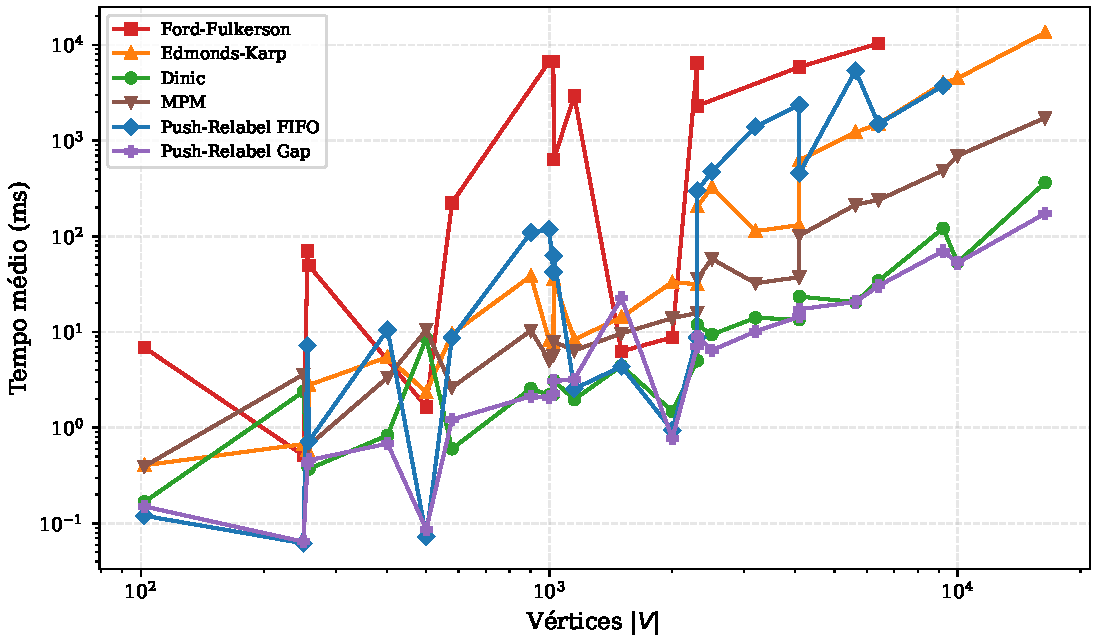
\includegraphics[width=0.92\textwidth]{book/figures/scalability_maxflow}
    \caption{Escalabilidade dos algoritmos de fluxo máximo em função de $|V|$ (escala log-log).}
    \label{fig:scalability_maxflow}
\end{figure}
}{}

\IfFileExists{book/figures/bars_maxflow.pdf}{
\begin{figure}[!ht]
    \centering
    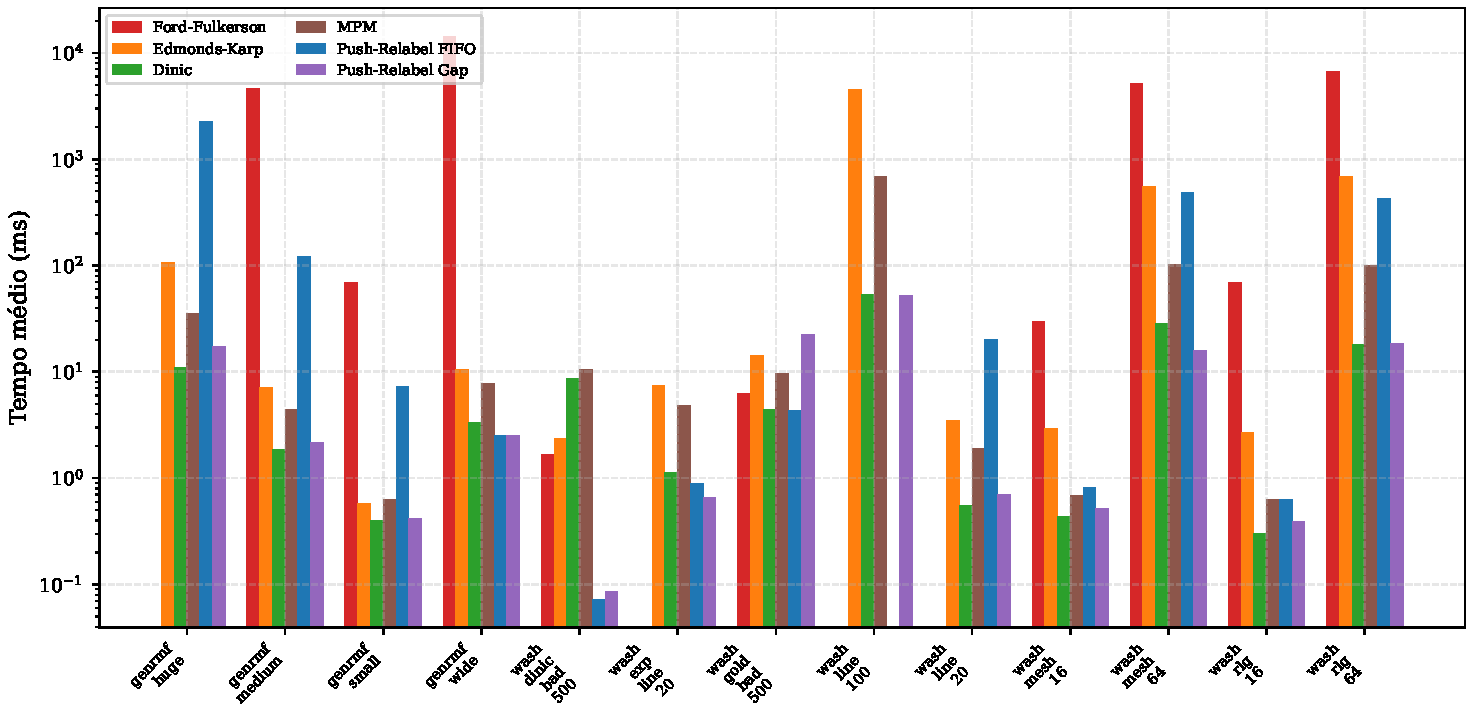
\includegraphics[width=0.98\textwidth]{book/figures/bars_maxflow}
    \caption{Comparação direta dos tempos médios de execução por instância (algoritmos de fluxo máximo).}
    \label{fig:bars_maxflow}
\end{figure}
}{}


\section{Resultados Experimentais: Fluxo de Custo Mínimo}\label{sec:bench_resultados_mincost}

A Tabela~\ref{tab:results_mincost} apresenta os resultados para os algoritmos de fluxo de custo mínimo nas 40 instâncias de referência Netgen da suíte DIMACS, reportando o custo ótimo $z^*$ e o menor tempo por instância em \textbf{negrito}.

\IfFileExists{book/tables/table_min_cost.tex}{
\begingroup
\small
\setlength{\tabcolsep}{4pt}
\begin{longtable}{llrrrrrrl}
\caption{Resultados experimentais dos motores de fluxo de custo mínimo.}\label{tab:results_mincost}\\
\toprule
\textbf{Instância} & \textbf{Algoritmo} & $|V|$ & $|A|$ & $f^*$ & $z^*$ & $\bar{t}$ (ms) & \textbf{Status} \\
\midrule
\endfirsthead
\caption[]{Resultados experimentais dos motores de fluxo de custo mínimo (continuação)}\\
\toprule
\textbf{Instância} & \textbf{Algoritmo} & $|V|$ & $|A|$ & $f^*$ & $z^*$ & $\bar{t}$ (ms) & \textbf{Status} \\
\midrule
\endhead
\bottomrule
\endfoot
netgen\_01.min & NetworkSimplex & 202 & 1508 & 100000 & 196587626 & \textbf{3.42} & OK \\
netgen\_01.min & SuccessiveShortestDijkstra & 202 & 1508 & 100000 & 196587626 & 9.06 & OK \\
netgen\_01.min & SuccessiveShortest & 202 & 1508 & 100000 & 196587626 & 5.27 & OK \\
netgen\_01.min & CycleCanceling & 202 & 1508 & 100000 & 196587626 & 215.56 & OK \\
\midrule
netgen\_02.min & NetworkSimplex & 202 & 1711 & 100000 & 194072029 & \textbf{2.58} & OK \\
netgen\_02.min & SuccessiveShortestDijkstra & 202 & 1711 & 100000 & 194072029 & 8.45 & OK \\
netgen\_02.min & SuccessiveShortest & 202 & 1711 & 100000 & 194072029 & 4.79 & OK \\
netgen\_02.min & CycleCanceling & 202 & 1711 & 100000 & 194072029 & 259.68 & OK \\
\midrule
netgen\_03.min & NetworkSimplex & 202 & 2200 & 100000 & 159442947 & \textbf{3.65} & OK \\
netgen\_03.min & SuccessiveShortestDijkstra & 202 & 2200 & 100000 & 159442947 & 10.41 & OK \\
netgen\_03.min & SuccessiveShortest & 202 & 2200 & 100000 & 159442947 & 7.30 & OK \\
netgen\_03.min & CycleCanceling & 202 & 2200 & 100000 & 159442947 & 387.21 & OK \\
\midrule
netgen\_04.min & NetworkSimplex & 202 & 2400 & 100000 & 138936551 & \textbf{3.66} & OK \\
netgen\_04.min & SuccessiveShortestDijkstra & 202 & 2400 & 100000 & 138936551 & 10.25 & OK \\
netgen\_04.min & SuccessiveShortest & 202 & 2400 & 100000 & 138936551 & 7.15 & OK \\
netgen\_04.min & CycleCanceling & 202 & 2400 & 100000 & 138936551 & 455.97 & OK \\
\midrule
netgen\_05.min & NetworkSimplex & 202 & 3100 & 100000 & 102950805 & \textbf{4.11} & OK \\
netgen\_05.min & SuccessiveShortestDijkstra & 202 & 3100 & 100000 & 102950805 & 13.48 & OK \\
netgen\_05.min & SuccessiveShortest & 202 & 3100 & 100000 & 102950805 & 10.68 & OK \\
netgen\_05.min & CycleCanceling & 202 & 3100 & 100000 & 102950805 & 739.45 & OK \\
\midrule
netgen\_06.min & NetworkSimplex & 302 & 3474 & 150000 & 191968577 & \textbf{6.94} & OK \\
netgen\_06.min & SuccessiveShortestDijkstra & 302 & 3474 & 150000 & 191968577 & 26.27 & OK \\
netgen\_06.min & SuccessiveShortest & 302 & 3474 & 150000 & 191968577 & 18.49 & OK \\
netgen\_06.min & CycleCanceling & 302 & 3474 & 150000 & 191968577 & 1568.24 & OK \\
\midrule
netgen\_07.min & NetworkSimplex & 302 & 4819 & 150000 & 172742047 & \textbf{10.05} & OK \\
netgen\_07.min & SuccessiveShortestDijkstra & 302 & 4819 & 150000 & 172742047 & 29.67 & OK \\
netgen\_07.min & SuccessiveShortest & 302 & 4819 & 150000 & 172742047 & 24.84 & OK \\
netgen\_07.min & CycleCanceling & 302 & 4819 & 150000 & 172742047 & 2744.12 & OK \\
\midrule
netgen\_08.min & NetworkSimplex & 302 & 5469 & 150000 & 177575586 & \textbf{10.86} & OK \\
netgen\_08.min & SuccessiveShortestDijkstra & 302 & 5469 & 150000 & 177575586 & 30.33 & OK \\
netgen\_08.min & SuccessiveShortest & 302 & 5469 & 150000 & 177575586 & 26.47 & OK \\
netgen\_08.min & CycleCanceling & 302 & 5469 & 150000 & 177575586 & 3306.26 & OK \\
\midrule
netgen\_09.min & NetworkSimplex & 302 & 6375 & 150000 & 144994180 & \textbf{12.75} & OK \\
netgen\_09.min & SuccessiveShortestDijkstra & 302 & 6375 & 150000 & 144994180 & 32.63 & OK \\
netgen\_09.min & SuccessiveShortest & 302 & 6375 & 150000 & 144994180 & 28.13 & OK \\
netgen\_09.min & CycleCanceling & 302 & 6375 & 150000 & 144994180 & 5569.99 & OK \\
\midrule
netgen\_10.min & NetworkSimplex & 302 & 6620 & 150000 & 148675665 & \textbf{12.78} & OK \\
netgen\_10.min & SuccessiveShortestDijkstra & 302 & 6620 & 150000 & 148675665 & 36.42 & OK \\
netgen\_10.min & SuccessiveShortest & 302 & 6620 & 150000 & 148675665 & 35.98 & OK \\
netgen\_10.min & CycleCanceling & 302 & 6620 & 150000 & 148675665 & 5255.40 & OK \\
\midrule
netgen\_11.min & NetworkSimplex & 402 & 1500 & 0 & 0 & 0.31 & OK \\
netgen\_11.min & SuccessiveShortestDijkstra & 402 & 1500 & 0 & 0 & 0.23 & OK \\
netgen\_11.min & SuccessiveShortest & 402 & 1500 & 0 & 0 & \textbf{0.18} & OK \\
netgen\_11.min & CycleCanceling & 402 & 1500 & 0 & 0 & 0.53 & OK \\
\midrule
netgen\_12.min & NetworkSimplex & 402 & 2250 & 0 & 0 & 0.40 & OK \\
netgen\_12.min & SuccessiveShortestDijkstra & 402 & 2250 & 0 & 0 & 0.29 & OK \\
netgen\_12.min & SuccessiveShortest & 402 & 2250 & 0 & 0 & \textbf{0.28} & OK \\
netgen\_12.min & CycleCanceling & 402 & 2250 & 0 & 0 & 0.81 & OK \\
\midrule
netgen\_13.min & NetworkSimplex & 402 & 3000 & 0 & 0 & 0.35 & OK \\
netgen\_13.min & SuccessiveShortestDijkstra & 402 & 3000 & 0 & 0 & 0.30 & OK \\
netgen\_13.min & SuccessiveShortest & 402 & 3000 & 0 & 0 & \textbf{0.29} & OK \\
netgen\_13.min & CycleCanceling & 402 & 3000 & 0 & 0 & 1.02 & OK \\
\midrule
netgen\_14.min & NetworkSimplex & 402 & 3750 & 0 & 0 & 0.57 & OK \\
netgen\_14.min & SuccessiveShortestDijkstra & 402 & 3750 & 0 & 0 & 0.33 & OK \\
netgen\_14.min & SuccessiveShortest & 402 & 3750 & 0 & 0 & \textbf{0.29} & OK \\
netgen\_14.min & CycleCanceling & 402 & 3750 & 0 & 0 & 1.34 & OK \\
\midrule
netgen\_15.min & NetworkSimplex & 402 & 4500 & 0 & 0 & 0.47 & OK \\
netgen\_15.min & SuccessiveShortestDijkstra & 402 & 4500 & 0 & 0 & \textbf{0.44} & OK \\
netgen\_15.min & SuccessiveShortest & 402 & 4500 & 0 & 0 & 0.47 & OK \\
netgen\_15.min & CycleCanceling & 402 & 4500 & 0 & 0 & 1.71 & OK \\
\midrule
netgen\_16.min & NetworkSimplex & 402 & 1374 & 400000 & 6815524469 & \textbf{2.49} & OK \\
netgen\_16.min & SuccessiveShortestDijkstra & 402 & 1374 & 400000 & 6815524469 & 5.70 & OK \\
netgen\_16.min & SuccessiveShortest & 402 & 1374 & 400000 & 6815524469 & 3.91 & OK \\
netgen\_16.min & CycleCanceling & 402 & 1374 & 400000 & 6815524469 & 75.16 & OK \\
\midrule
netgen\_17.min & NetworkSimplex & 402 & 2511 & 400000 & 2646770386 & \textbf{3.81} & OK \\
netgen\_17.min & SuccessiveShortestDijkstra & 402 & 2511 & 400000 & 2646770386 & 6.01 & OK \\
netgen\_17.min & SuccessiveShortest & 402 & 2511 & 400000 & 2646770386 & 4.07 & OK \\
netgen\_17.min & CycleCanceling & 402 & 2511 & 400000 & 2646770386 & 204.99 & OK \\
\midrule
netgen\_18.min & NetworkSimplex & 402 & 1374 & 400000 & 6663684919 & \textbf{2.49} & OK \\
netgen\_18.min & SuccessiveShortestDijkstra & 402 & 1374 & 400000 & 6663684919 & 5.21 & OK \\
netgen\_18.min & SuccessiveShortest & 402 & 1374 & 400000 & 6663684919 & 3.45 & OK \\
netgen\_18.min & CycleCanceling & 402 & 1374 & 400000 & 6663684919 & 80.27 & OK \\
\midrule
netgen\_19.min & NetworkSimplex & 402 & 2511 & 400000 & 2618979806 & \textbf{3.67} & OK \\
netgen\_19.min & SuccessiveShortestDijkstra & 402 & 2511 & 400000 & 2618979806 & 6.01 & OK \\
netgen\_19.min & SuccessiveShortest & 402 & 2511 & 400000 & 2618979806 & 4.14 & OK \\
netgen\_19.min & CycleCanceling & 402 & 2511 & 400000 & 2618979806 & 209.40 & OK \\
\midrule
netgen\_20.min & NetworkSimplex & 402 & 1484 & 400000 & 6749969302 & \textbf{2.49} & OK \\
netgen\_20.min & SuccessiveShortestDijkstra & 402 & 1484 & 400000 & 6749969302 & 5.25 & OK \\
netgen\_20.min & SuccessiveShortest & 402 & 1484 & 400000 & 6749969302 & 3.07 & OK \\
netgen\_20.min & CycleCanceling & 402 & 1484 & 400000 & 6749969302 & 117.08 & OK \\
\midrule
netgen\_21.min & NetworkSimplex & 402 & 2904 & 400000 & 2631027973 & \textbf{3.42} & OK \\
netgen\_21.min & SuccessiveShortestDijkstra & 402 & 2904 & 400000 & 2631027973 & 6.34 & OK \\
netgen\_21.min & SuccessiveShortest & 402 & 2904 & 400000 & 2631027973 & 4.22 & OK \\
netgen\_21.min & CycleCanceling & 402 & 2904 & 400000 & 2631027973 & 271.33 & OK \\
\midrule
netgen\_22.min & NetworkSimplex & 402 & 1484 & 400000 & 6621515104 & 2.47 & OK \\
netgen\_22.min & SuccessiveShortestDijkstra & 402 & 1484 & 400000 & 6621515104 & 4.49 & OK \\
netgen\_22.min & SuccessiveShortest & 402 & 1484 & 400000 & 6621515104 & \textbf{2.42} & OK \\
netgen\_22.min & CycleCanceling & 402 & 1484 & 400000 & 6621515104 & 110.87 & OK \\
\midrule
netgen\_23.min & NetworkSimplex & 402 & 2904 & 400000 & 2630071408 & \textbf{3.50} & OK \\
netgen\_23.min & SuccessiveShortestDijkstra & 402 & 2904 & 400000 & 2630071408 & 6.49 & OK \\
netgen\_23.min & SuccessiveShortest & 402 & 2904 & 400000 & 2630071408 & 4.31 & OK \\
netgen\_23.min & CycleCanceling & 402 & 2904 & 400000 & 2630071408 & 255.31 & OK \\
\midrule
netgen\_24.min & NetworkSimplex & 402 & 1398 & 400000 & 6829799687 & 2.44 & OK \\
netgen\_24.min & SuccessiveShortestDijkstra & 402 & 1398 & 400000 & 6829799687 & 3.09 & OK \\
netgen\_24.min & SuccessiveShortest & 402 & 1398 & 400000 & 6829799687 & \textbf{2.29} & OK \\
netgen\_24.min & CycleCanceling & 402 & 1398 & 400000 & 6829799687 & 57.83 & OK \\
\midrule
netgen\_25.min & NetworkSimplex & 402 & 2692 & 400000 & 6396423129 & \textbf{3.47} & OK \\
netgen\_25.min & SuccessiveShortestDijkstra & 402 & 2692 & 400000 & 6396423129 & 7.27 & OK \\
netgen\_25.min & SuccessiveShortest & 402 & 2692 & 400000 & 6396423129 & 6.00 & OK \\
netgen\_25.min & CycleCanceling & 402 & 2692 & 400000 & 6396423129 & 166.21 & OK \\
\midrule
netgen\_26.min & NetworkSimplex & 402 & 1398 & 400000 & 5297702923 & 1.94 & OK \\
netgen\_26.min & SuccessiveShortestDijkstra & 402 & 1398 & 400000 & 5297702923 & 1.36 & OK \\
netgen\_26.min & SuccessiveShortest & 402 & 1398 & 400000 & 5297702923 & \textbf{0.69} & OK \\
netgen\_26.min & CycleCanceling & 402 & 1398 & 400000 & 5297702923 & 19.78 & OK \\
\midrule
netgen\_27.min & NetworkSimplex & 402 & 2692 & 400000 & 4863992745 & 3.20 & OK \\
netgen\_27.min & SuccessiveShortestDijkstra & 402 & 2692 & 400000 & 4863992745 & 3.49 & OK \\
netgen\_27.min & SuccessiveShortest & 402 & 2692 & 400000 & 4863992745 & \textbf{2.81} & OK \\
netgen\_27.min & CycleCanceling & 402 & 2692 & 400000 & 4863992745 & 87.80 & OK \\
\midrule
netgen\_28.min & NetworkSimplex & 1002 & 3000 & 1000000 & 11599233408 & 16.84 & OK \\
netgen\_28.min & SuccessiveShortestDijkstra & 1002 & 3000 & 1000000 & 11599233408 & 16.46 & OK \\
netgen\_28.min & SuccessiveShortest & 1002 & 3000 & 1000000 & 11599233408 & \textbf{13.00} & OK \\
netgen\_28.min & CycleCanceling & 1002 & 3000 & 1000000 & 11599233408 & 1102.81 & OK \\
\midrule
netgen\_29.min & NetworkSimplex & 1002 & 3500 & 1000000 & 11700773092 & 18.83 & OK \\
netgen\_29.min & SuccessiveShortestDijkstra & 1002 & 3500 & 1000000 & 11700773092 & 21.39 & OK \\
netgen\_29.min & SuccessiveShortest & 1002 & 3500 & 1000000 & 11700773092 & \textbf{17.36} & OK \\
netgen\_29.min & CycleCanceling & 1002 & 3500 & 1000000 & 11700773092 & 1145.25 & OK \\
\midrule
netgen\_30.min & NetworkSimplex & 1002 & 4500 & 1000000 & 8782721260 & 23.33 & OK \\
netgen\_30.min & SuccessiveShortestDijkstra & 1002 & 4500 & 1000000 & 8782721260 & 24.64 & OK \\
netgen\_30.min & SuccessiveShortest & 1002 & 4500 & 1000000 & 8782721260 & \textbf{22.69} & OK \\
netgen\_30.min & CycleCanceling & 1002 & 4500 & 1000000 & 8782721260 & 1989.27 & OK \\
\midrule
netgen\_31.min & NetworkSimplex & 1002 & 4900 & 1000000 & 8577913734 & 26.10 & OK \\
netgen\_31.min & SuccessiveShortestDijkstra & 1002 & 4900 & 1000000 & 8577913734 & 27.70 & OK \\
netgen\_31.min & SuccessiveShortest & 1002 & 4900 & 1000000 & 8577913734 & \textbf{21.53} & OK \\
netgen\_31.min & CycleCanceling & 1002 & 4900 & 1000000 & 8577913734 & 1766.12 & OK \\
\midrule
netgen\_32.min & NetworkSimplex & 1502 & 4492 & 1500000 & 17996365110 & 40.75 & OK \\
netgen\_32.min & SuccessiveShortestDijkstra & 1502 & 4492 & 1500000 & 17996365110 & 41.66 & OK \\
netgen\_32.min & SuccessiveShortest & 1502 & 4492 & 1500000 & 17996365110 & \textbf{37.16} & OK \\
netgen\_32.min & CycleCanceling & 1502 & 4492 & 1500000 & 17996365110 & 5639.30 & OK \\
\midrule
netgen\_33.min & NetworkSimplex & 1502 & 4535 & 1500000 & 18424893900 & \textbf{44.59} & OK \\
netgen\_33.min & SuccessiveShortestDijkstra & 1502 & 4535 & 1500000 & 18424893900 & 44.63 & OK \\
netgen\_33.min & SuccessiveShortest & 1502 & 4535 & 1500000 & 18424893900 & 44.62 & OK \\
netgen\_33.min & CycleCanceling & 1502 & 4535 & 1500000 & 18424893900 & 5172.76 & OK \\
\midrule
netgen\_34.min & NetworkSimplex & 1502 & 5257 & 1500000 & 14596094907 & 52.30 & OK \\
netgen\_34.min & SuccessiveShortestDijkstra & 1502 & 5257 & 1500000 & 14596094907 & 42.97 & OK \\
netgen\_34.min & SuccessiveShortest & 1502 & 5257 & 1500000 & 14596094907 & \textbf{40.19} & OK \\
netgen\_34.min & CycleCanceling & 1502 & 5257 & 1500000 & 14596094907 & 6407.65 & OK \\
\midrule
netgen\_35.min & NetworkSimplex & 1502 & 5880 & 1500000 & 14350903861 & \textbf{53.26} & OK \\
netgen\_35.min & SuccessiveShortestDijkstra & 1502 & 5880 & 1500000 & 14350903861 & 59.49 & OK \\
netgen\_35.min & SuccessiveShortest & 1502 & 5880 & 1500000 & 14350903861 & 62.66 & OK \\
netgen\_35.min & CycleCanceling & 1502 & 5880 & 1500000 & 14350903861 & 8420.28 & OK \\
\midrule
netgen\_36.min & NetworkSimplex & 8002 & 16200 & 4000000 & 87957673940 & \textbf{1775.15} & OK \\
netgen\_36.min & SuccessiveShortestDijkstra & 8002 & 16200 & 4000000 & 87957673940 & 2069.65 & OK \\
netgen\_36.min & SuccessiveShortest & 8002 & 16200 & 4000000 & 87957673940 & 2942.66 & OK \\
netgen\_36.min & CycleCanceling & 8002 & 16200 & -1 & -1 & --- & TLE \\
\midrule
netgen\_37.min & NetworkSimplex & 5002 & 23950 & 4000000 & 35607266430 & \textbf{1490.74} & OK \\
netgen\_37.min & SuccessiveShortestDijkstra & 5002 & 23950 & 4000000 & 35607266430 & 1712.00 & OK \\
netgen\_37.min & SuccessiveShortest & 5002 & 23950 & 4000000 & 35607266430 & 2589.79 & OK \\
netgen\_37.min & CycleCanceling & 5002 & 23950 & -1 & -1 & --- & TLE \\
\midrule
netgen\_38.min & NetworkSimplex & 3002 & 35625 & 2000000 & 7265734372 & \textbf{756.55} & OK \\
netgen\_38.min & SuccessiveShortestDijkstra & 3002 & 35625 & 2000000 & 7265734372 & 1104.99 & OK \\
netgen\_38.min & SuccessiveShortest & 3002 & 35625 & 2000000 & 7265734372 & 1773.57 & OK \\
netgen\_38.min & CycleCanceling & 3002 & 35625 & -1 & -1 & --- & TLE \\
\midrule
netgen\_39.min & NetworkSimplex & 5002 & 15880 & 4000000 & 48660418428 & \textbf{887.09} & OK \\
netgen\_39.min & SuccessiveShortestDijkstra & 5002 & 15880 & 4000000 & 48660418428 & 1224.72 & OK \\
netgen\_39.min & SuccessiveShortest & 5002 & 15880 & 4000000 & 48660418428 & 1581.67 & OK \\
netgen\_39.min & CycleCanceling & 5002 & 15880 & -1 & -1 & --- & TLE \\
\midrule
netgen\_40.min & NetworkSimplex & 3002 & 23400 & 2000000 & 11068572024 & \textbf{475.23} & OK \\
netgen\_40.min & SuccessiveShortestDijkstra & 3002 & 23400 & 2000000 & 11068572024 & 550.14 & OK \\
netgen\_40.min & SuccessiveShortest & 3002 & 23400 & 2000000 & 11068572024 & 763.12 & OK \\
netgen\_40.min & CycleCanceling & 3002 & 23400 & -1 & -1 & --- & TLE \\
\end{longtable}
\endgroup

}{}

\IfFileExists{book/figures/scalability_mincost.pdf}{
\begin{figure}[!ht]
    \centering
    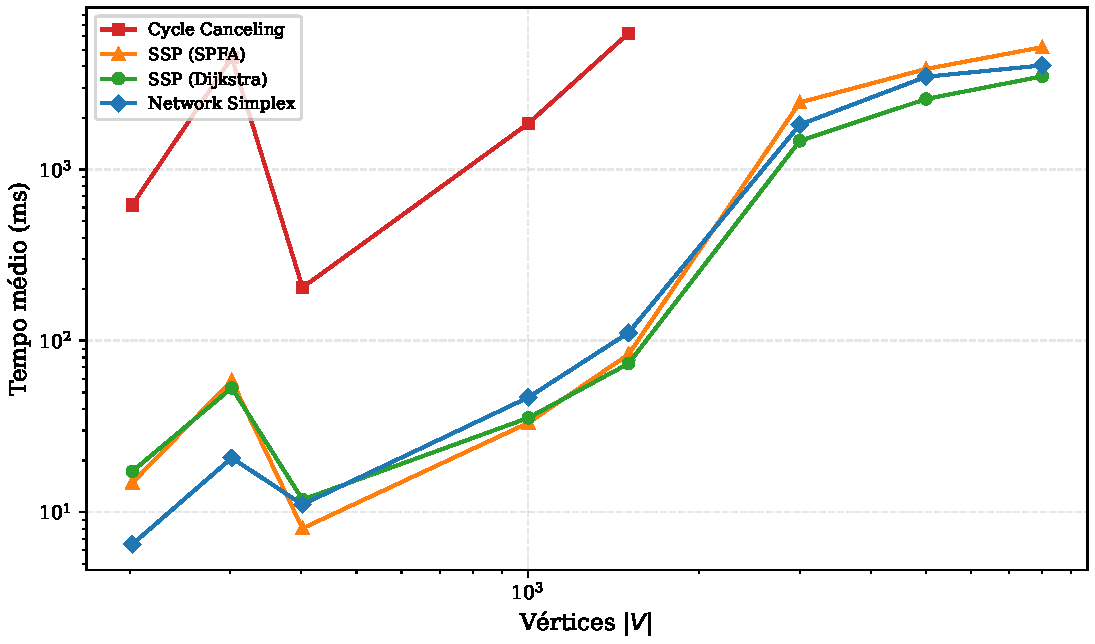
\includegraphics[width=0.92\textwidth]{book/figures/scalability_mincost}
    \caption{Escalabilidade dos algoritmos de fluxo de custo mínimo em função de $|V|$ (escala log-log).}
    \label{fig:scalability_mincost}
\end{figure}
}{}

\IfFileExists{book/figures/bars_mincost.pdf}{
\begin{figure}[!ht]
    \centering
    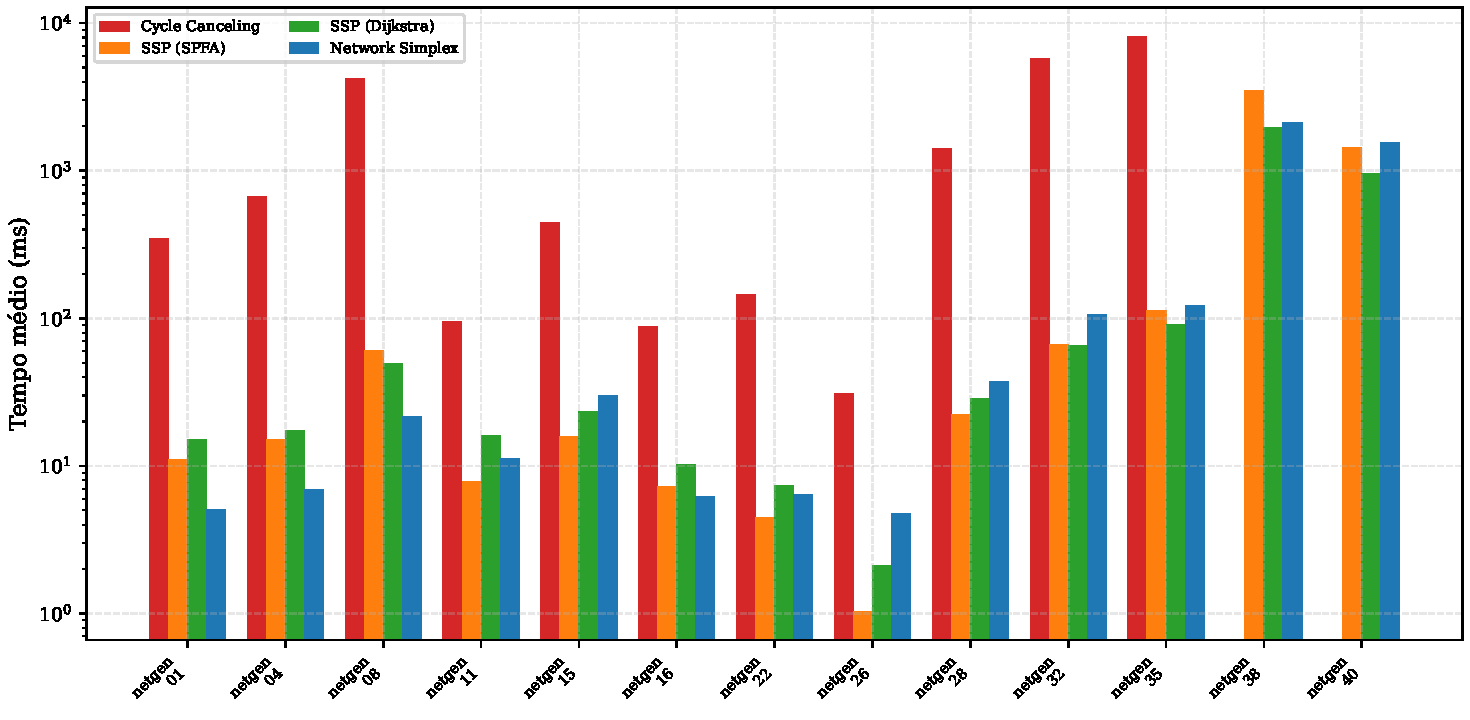
\includegraphics[width=0.98\textwidth]{book/figures/bars_mincost}
    \caption{Comparação direta dos tempos médios de execução por instância (algoritmos de fluxo de custo mínimo).}
    \label{fig:bars_mincost}
\end{figure}
}{}


\section{Resultados Experimentais: Emparelhamento e Atribuição Bipartida}\label{sec:bench_resultados_bipartite}

Para quantificar o ganho prático das estruturas dedicadas em relação às reduções gerais de fluxo, avaliaram-se os motores \lstinline{Kuhn} e \lstinline{HopcroftKarp} frente aos seis motores de fluxo máximo nas 10 instâncias de emparelhamento bipartido (Tabela~\ref{tab:benchmarks_bipartite_matching} e Figura~\ref{fig:bars_bipartite_matching}), bem como o algoritmo Húngaro (\lstinline{KuhnMunkres}) frente aos quatro motores de custo mínimo nas 8 instâncias de atribuição ponderada (Tabela~\ref{tab:benchmarks_bipartite_assignment} e Figura~\ref{fig:bars_bipartite_assignment}).

\IfFileExists{book/tables/table_bipartite_matching.tex}{
\begin{table}[!ht]
\centering
\small
\setlength{\tabcolsep}{3.5pt}
\begin{tabular}{lrrrrrrrrrrr}
\toprule
\textbf{Instância} & $|V|$ & $|A|$ & $|M^*|$ & \textbf{HK} & \textbf{Kuhn} & \textbf{Dinic} & \textbf{PR-Gap} & \textbf{MPM} & \textbf{PR} & \textbf{EK} & \textbf{FF} \\
\midrule
\texttt{bip\_dense\_1000} & 2.002 & 152.751 & 1.000 & 20,7 & 76,4 & \textbf{18,4} & 23,4 & 30,4 & 19,5 & 205 & 206 \\
\texttt{bip\_dense\_300} & 602 & 23.620 & 300 & 4,70 & 5,66 & \textbf{2,98} & 4,07 & 5,75 & 4,12 & 12,7 & 13,1 \\
\texttt{bip\_dense\_600} & 1.202 & 73.471 & 600 & \textbf{10,6} & 27,3 & 12,0 & 10,9 & 16,1 & 11,2 & 56,2 & 57,4 \\
\texttt{bip\_regular\_1200} & 2.402 & 20.400 & 1.200 & 5,08 & 18,3 & \textbf{3,53} & 3,58 & 11,7 & 4,68 & 37,5 & 49,1 \\
\texttt{bip\_sparse\_1000} & 2.002 & 12.000 & 1.000 & 2,98 & 8,89 & 3,00 & \textbf{2,98} & 8,92 & 3,61 & 22,1 & 18,8 \\
\texttt{bip\_sparse\_2000} & 4.002 & 28.000 & 2.000 & 5,95 & 41,3 & \textbf{5,52} & 5,93 & 24,1 & 6,81 & 93,0 & 119 \\
\texttt{bip\_sparse\_500} & 1.002 & 5.000 & 500 & 2,50 & 2,44 & \textbf{0,63} & 1,27 & 2,64 & 1,10 & 5,72 & 4,90 \\
\texttt{bip\_trap\_1000} & 2.002 & 11.770 & 1.000 & 1,72 & 12,9 & \textbf{1,25} & 25,4 & 6,75 & 29,3 & 20,3 & 29,5 \\
\texttt{bip\_trap\_1500} & 3.002 & 17.718 & 1.500 & 4,37 & 26,8 & \textbf{4,34} & 60,9 & 15,3 & 64,3 & 45,8 & 76,5 \\
\texttt{bip\_trap\_500} & 1.002 & 4.858 & 500 & \textbf{1,07} & 3,08 & 1,29 & 5,65 & 3,08 & 6,38 & 5,50 & 6,38 \\
\bottomrule
\end{tabular}
\caption{Comparação experimental entre algoritmos dedicados (Kuhn e Hopcroft-Karp) e motores gerais de fluxo máximo em instâncias de emparelhamento bipartido (tempos médios em ms).}
\label{tab:benchmarks_bipartite_matching}
\end{table}

}{}

\IfFileExists{book/figures/bars_bipartite_matching.pdf}{
\begin{figure}[!ht]
    \centering
    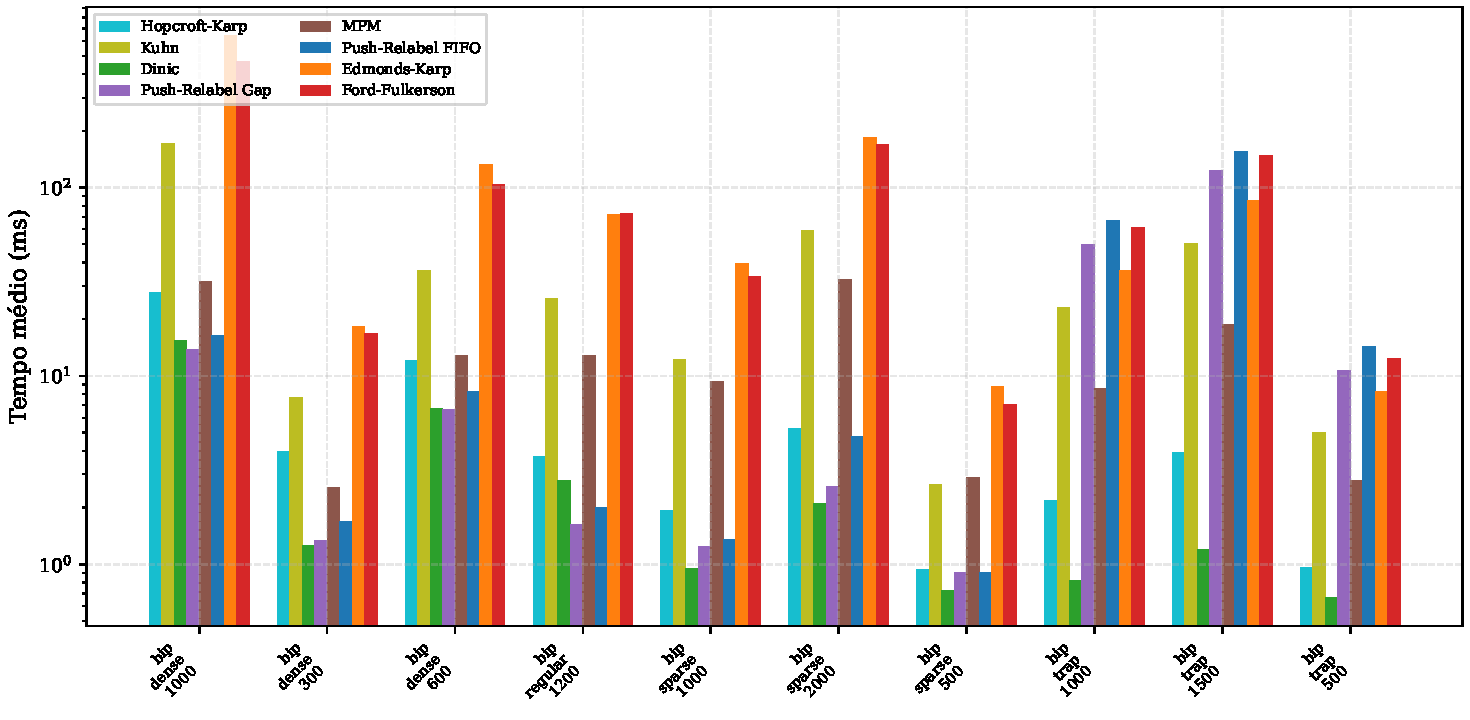
\includegraphics[width=0.95\textwidth]{book/figures/bars_bipartite_matching}
    \caption{Tempos médios de execução nas instâncias de emparelhamento bipartido máximo: algoritmos dedicados (\texttt{HopcroftKarp} e \texttt{Kuhn}) versus motores gerais de fluxo máximo.}
    \label{fig:bars_bipartite_matching}
\end{figure}
}{}

\IfFileExists{book/tables/table_bipartite_assignment.tex}{
\begin{table}[!ht]
\centering
\small
\setlength{\tabcolsep}{3.5pt}
\begin{tabular}{lrrrrrrrr}
\toprule
\textbf{Instância} & $|V|$ & $|A|$ & $z^*$ & \textbf{Húngaro} & \textbf{Simplex} & \textbf{SSP-Dijk} & \textbf{SSP-SPFA} & \textbf{CC} \\
\midrule
\texttt{assign\_euclid\_150} & 302 & 22.800 & 113.735 & \textbf{3,79} & 56,4 & 22,5 & 25,8 & 2.374 \\
\texttt{assign\_euclid\_220} & 442 & 48.840 & 163.859 & \textbf{8,27} & 162 & 72,5 & 104 & 15.642 \\
\texttt{assign\_highcost\_150} & 302 & 22.800 & 1.889.344 & \textbf{4,58} & 51,0 & 24,4 & 23,9 & 1.970 \\
\texttt{assign\_highcost\_220} & 442 & 48.840 & 1.638.938 & \textbf{7,67} & 176 & 67,9 & 77,5 & 13.396 \\
\texttt{assign\_uniform\_120} & 242 & 14.640 & 1.715 & \textbf{1,84} & 24,2 & 11,8 & 10,0 & 650 \\
\texttt{assign\_uniform\_180} & 362 & 32.760 & 1.890 & \textbf{5,30} & 92,7 & 39,6 & 41,8 & 5.327 \\
\texttt{assign\_uniform\_240} & 482 & 58.080 & 1.795 & \textbf{7,67} & 212 & 92,9 & 102 & 19.576 \\
\texttt{assign\_uniform\_80} & 162 & 6.560 & 1.548 & \textbf{1,12} & 7,01 & 4,83 & 3,39 & 135 \\
\bottomrule
\end{tabular}
\caption{Comparação experimental entre o algoritmo Húngaro (Kuhn-Munkres) e motores gerais de fluxo de custo mínimo em instâncias de atribuição bipartida (tempos médios em ms).}
\label{tab:benchmarks_bipartite_assignment}
\end{table}

}{}

\IfFileExists{book/figures/bars_bipartite_assignment.pdf}{
\begin{figure}[!ht]
    \centering
    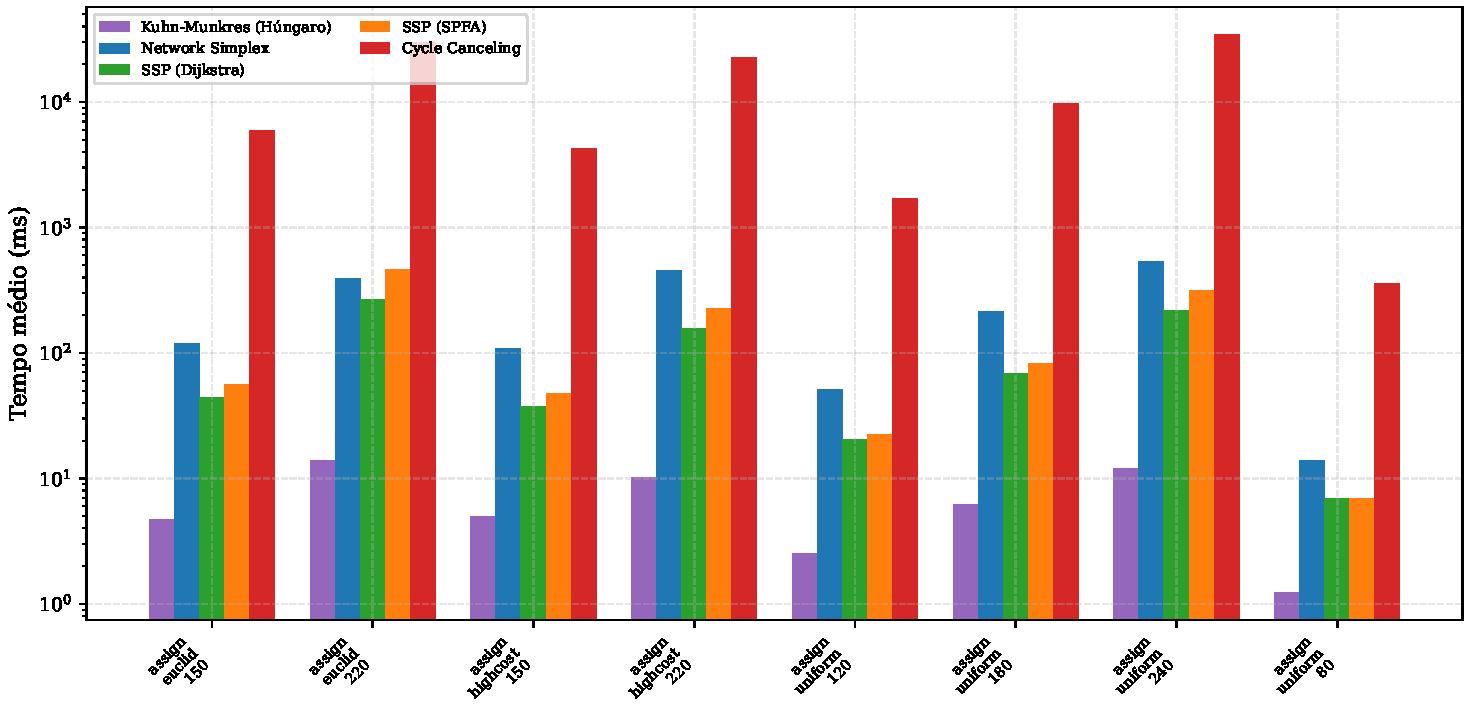
\includegraphics[width=0.95\textwidth]{book/figures/bars_bipartite_assignment}
    \caption{Tempos médios de execução nas instâncias de atribuição bipartida ponderada: algoritmo Húngaro (\texttt{KuhnMunkres}) versus motores gerais de fluxo de custo mínimo.}
    \label{fig:bars_bipartite_assignment}
\end{figure}
}{}

Observa-se que \lstinline{HopcroftKarp} atinge os menores tempos em todas as instâncias de emparelhamento bipartido, beneficiando-se da ausência de manipulação explícita dos arcos da fonte e do sorvedouro durante as fases de busca, seguido de perto por \lstinline{Dinic}. Analogamente, nas instâncias densas de atribuição bipartida, \lstinline{KuhnMunkres} supera os algoritmos gerais de fluxo de custo mínimo ao atualizar os potenciais duais diretamente sobre a matriz compacta em $\mathcal{O}(|V|^3)$.


% =========================================================================
% EPÍLOGO DO LIVRO: SÍNTESE E HORIZONTES DE PESQUISA
% =========================================================================
\chapter*{Epílogo: Síntese e Horizontes de Pesquisa}\label{sec:conclusoes}
\addcontentsline{toc}{chapter}{Epílogo: Síntese e Horizontes de Pesquisa}

Os resultados e implementações consolidados neste volume integram a teoria matemática da Otimização Combinatória à engenharia de software em C++23. O texto estruturou-se em quatro eixos:

\begin{enumerate}[leftmargin=1.5em, itemsep=0.4em]
    \item \textbf{Fundamentação Teórica:} Demonstração matemática dos teoremas estruturais de fluxo (Fluxo Máximo e Corte Mínimo, Integralidade, Decomposição de Fluxo, Teoremas de Menger, König e as Quatro Dualidades em grafos bipartidos; e, em custo mínimo, otimalidade por ciclos negativos, custos reduzidos, folga complementar e Total Unimodularidade da matriz de incidência).

    \item \textbf{Arquitetura em C++23:} Desenvolvimento de classes base abstratas e 13 algoritmos especializados divididos em duas famílias:
    \begin{itemize}
        \item \textbf{Família \lstinline{FlowNetwork} (Fluxo Máximo e Emparelhamento Bipartido):} \lstinline{FordFulkerson}, \lstinline{EdmondsKarp}, \lstinline{Dinic}, \lstinline{MPM}, \lstinline{PushRelabel} (FIFO), \lstinline{PushRelabelImproved} (Gap Heuristic), \lstinline{Kuhn} e \lstinline{HopcroftKarp}.
        \item \textbf{Família \lstinline{CostNetwork} (Custo Mínimo e Atribuição Bipartida):} \lstinline{CycleCanceling}, \lstinline{SuccessiveShortest} (SPFA), \lstinline{SuccessiveShortestDijkstra} (Potenciais), \lstinline{NetworkSimplex} e \lstinline{KuhnMunkres} (Algoritmo Húngaro).
    \end{itemize}

    \item \textbf{Reduções e Aplicações:} Resolução de problemas clássicos (\textit{Maximum Bipartite Matching}, \textit{Minimum Vertex Cover}, \textit{Maximum Independent Set}, caminhos disjuntos e corte mínimo) e aplicação em \textbf{Segmentação Interativa de Imagens} via corte mínimo em grafos (\textit{Graph Cuts}).

    \item \textbf{Avaliação Experimental:} Protocolo de medição de tempo de CPU sob isolamento em instâncias padronizadas da literatura (coleções DIMACS), validando a corretude das soluções por certificação cruzada.
\end{enumerate}

Como trabalhos futuros, destacam-se a avaliação empírica sobre grafos esparsos de grande porte, a implementação de versões paralelas em OpenMP para algoritmos de pré-fluxo e a exploração de regras de pivoteamento adicionais no \textit{Network Simplex} (como \textit{Candidate List Pricing}).




\backmatter

\bibliographystyle{plain}
\bibliography{common/references}

\appendix
\part{Apêndices e Implementações em C++23}

% =========================================================================
% ARQUITETURA DE SOFTWARE EM C++23 E ESTRUTURAS DE DADOS
% =========================================================================
\apendice{Arquitetura Orientada a Objetos em C++23 e Estruturas de Dados}
\label{ap:arquitetura}

A implementação dos modelos matemáticos abstratos em algoritmos computacionais de alto desempenho foi realizada no paradigma da Orientação a Objetos através do padrão ISO C++23.

\paragraph{Tipagem e Margem de Segurança Numérica.}
A biblioteca adota apelidos de tipo (\textit{Type Aliases}) padronizados: \lstinline{Long} (\lstinline{long long}) para capacidades e fluxos, e \lstinline{Size} (\lstinline{std::size_t}) para identificadores nodais e dimensionamento de estruturas de dados. Para mitigar o risco de estouro de inteiros (\textit{Integer Overflow}) em somas cumulativas de capacidades infinitas, as constantes de saturação são definidas com deslocamento defensivo de 8 bits à direita:
\begin{lstlisting}[language=C++, numbers=none, basicstyle=\ttfamily\footnotesize, frame=none, backgroundcolor=\color{white}]
constexpr Long INF = std::numeric_limits<Long>::max() >> 8;
constexpr Size MAX = std::numeric_limits<Size>::max() >> 8;
\end{lstlisting}

\paragraph{Representação Contígua de Grafo Residual e Emparelhamento XOR.}
Para favorecer a localidade de cache da CPU e eliminar o overhead de alocações dinâmicas dispersas, a estrutura de adjacência da rede é mantida em duas estruturas integradas:
\begin{enumerate}
    \item \lstinline{std::vector<Edge> edges}: vetor contíguo na memória contendo todas as conexões da rede (\lstinline{from}, \lstinline{to}, \lstinline{capacity}, \lstinline{flow});
    \item \lstinline{std::vector<std::vector<Size>> adj}: lista de adjacência onde cada entrada armazena apenas os índices numéricos dos arcos no vetor principal \lstinline{edges}.
\end{enumerate}

No método \lstinline{add_edge(u, v, cap, rev_cap)}, os arcos direto e reverso são alocados em pares sequenciais contíguos (índices $2k$ e $2k+1$). Consequentemente, o acesso ao arco residual simétrico opera em tempo estritamente $\mathcal{O}(1)$ via operador bit a bit Ou Exclusivo (\lstinline{id ^ 1ULL}):
\begin{lstlisting}[language=C++, numbers=none, basicstyle=\ttfamily\footnotesize, frame=none, backgroundcolor=\color{white}]
void push_flow(const Size edge_id, const Long flow_amount) {
    edges[edge_id].flow += flow_amount;
    edges[edge_id ^ 1ULL].flow -= flow_amount;
}
\end{lstlisting}

\paragraph{Hierarquia Polimórfica e Padrões de Projeto.}
A biblioteca organiza-se em duas famílias baseadas nos padrões \textit{Strategy}, \textit{Factory Method} e \textit{Prototype}~\cite{gamma1994design}:
\begin{itemize}
    \item \textbf{Família \lstinline{FlowNetwork} (Fluxo Máximo):} Interface base abstrata com o método virtual puro \lstinline{compute_max_flow(source, sink)}. Os algoritmos concretos (\lstinline{FordFulkerson}, \lstinline{EdmondsKarp}, \lstinline{Dinic}, \lstinline{MPM}, \lstinline{PushRelabel}, \lstinline{PushRelabelImproved}, \lstinline{Kuhn} e \lstinline{HopcroftKarp}) implementam estratégias de busca distintas mantendo total intercambialidade;
    \item \textbf{Família \lstinline{CostNetwork} (Custo Mínimo):} Interface base abstrata que incorpora o custo linear unitário $w$ aos arcos, com o método virtual puro \lstinline{compute_min_cost_max_flow(source, sink)} implementado por \lstinline{CycleCanceling}, \lstinline{SuccessiveShortest}, \lstinline{SuccessiveShortestDijkstra}, \lstinline{NetworkSimplex} e \lstinline{KuhnMunkres}.
\end{itemize}

Os métodos virtuais \lstinline{make(n)} e \lstinline{clone()} permitem a instanciação e a clonagem profunda (\textit{deep copy}) de instâncias polimórficas preservando o estado residual, o que é fundamental em aplicações iterativas como corte mínimo e segmentação de imagens.

\newpage

% =========================================================================
% IMPLEMENTAÇÃO DA INTERFACE BASE ``FLOW-NETWORK''
% =========================================================================
\apendice{Implementação da Interface Base ``Flow-Network''}
\label{ap:flownetwork}

\begin{lstlisting}[caption={Implementação em C++ da interface base \lstinline{FlowNetwork} para a modelagem abstrata de redes de fluxo.}, label={lst:flownetwork}]
#ifndef FLOW_NETWORK_HPP
#define FLOW_NETWORK_HPP

#include <limits>
#include <memory>
#include <vector>

using Long = long long;
using Size = std::size_t;

constexpr Long INF = std::numeric_limits<Long>::max() >> 8;
constexpr Size MAX = std::numeric_limits<Size>::max() >> 8;

class FlowNetwork
{
public:
	struct Edge
	{
		Size from, to;
		Long capacity, flow;
	};

	explicit FlowNetwork(const Size n) : size(n), adjacency(n) {}
	virtual ~FlowNetwork() = default;

	virtual std::unique_ptr<FlowNetwork> make(const Size n) const = 0;
	virtual std::unique_ptr<FlowNetwork> clone() const = 0;

	virtual void add_edge(
	    const Size from, const Size to, const Long capacity,
	    const Long reverse_capacity = 0
	)
	{
		adjacency[from].push_back(edges.size());
		edges.push_back({from, to, capacity, 0});
		adjacency[to].push_back(edges.size());
		edges.push_back({to, from, reverse_capacity, 0});
	}

	virtual Long compute_max_flow(const Size source, const Size sink) = 0;

	[[nodiscard]] Size get_size() const
	{
		return size;
	}

	[[nodiscard]] const std::vector<Edge> &get_edges() const
	{
		return edges;
	}

	[[nodiscard]] const std::vector<std::vector<Size>> &get_adjacency() const
	{
		return adjacency;
	}

protected:
	Size size;
	std::vector<Edge> edges;
	std::vector<std::vector<Size>> adjacency;

	[[nodiscard]] Long get_residual_capacity(const Size edge_id) const
	{
		return edges[edge_id].capacity - edges[edge_id].flow;
	}

	void push_flow(const Size edge_id, const Long flow_amount)
	{
		edges[edge_id].flow += flow_amount;
		edges[edge_id ^ 1ULL].flow -= flow_amount;
	}
};

#endif // FLOW_NETWORK_HPP
\end{lstlisting}

\newpage

% =========================================================================
% IMPLEMENTAÇÃO DA CLASSE ``FORD-FULKERSON''
% =========================================================================
\apendice{Implementação da Classe ``Ford-Fulkerson''}
\label{ap:ford_fulkerson}

\begin{lstlisting}[caption={Implementação em C++ da classe \lstinline{FordFulkerson}, método genérico de caminhos aumentantes via DFS.}, label={lst:ford_fulkerson}]
#ifndef FORD_FULKERSON_HPP
#define FORD_FULKERSON_HPP

#include "FlowNetwork.hpp"

class FordFulkerson : public FlowNetwork
{
public:
	explicit FordFulkerson(const Size n) : FlowNetwork(n), visited(n, 0), token(0) {}

	static std::unique_ptr<FlowNetwork> create(const Size n)
	{
		return std::make_unique<FordFulkerson>(n);
	}

	std::unique_ptr<FlowNetwork> make(const Size n) const override
	{
		return std::make_unique<FordFulkerson>(n);
	}

	std::unique_ptr<FlowNetwork> clone() const override
	{
		return std::make_unique<FordFulkerson>(*this);
	}

	Long compute_max_flow(const Size source, const Size sink) override
	{
		Long total_flow = 0;
		token = 0;

		while (true)
		{
			++token;
			const Long bottleneck = dfs(source, sink, INF);
			if (bottleneck == 0)
				break;
			total_flow += bottleneck;
		}

		return total_flow;
	}

private:
	std::vector<Size> visited;
	Size token;

	Long dfs(const Size current_node, const Size sink, const Long flow_pushed)
	{
		if (current_node == sink)
			return flow_pushed;

		visited[current_node] = token;

		for (const Size edge_id : adjacency[current_node])
		{
			const Size next_node = edges[edge_id].to;
			const Long residual_capacity = get_residual_capacity(edge_id);

			if (visited[next_node] == token || residual_capacity <= 0)
				continue;

			const Long bottleneck = std::min(flow_pushed, residual_capacity);
			const Long flow_transmitted = dfs(next_node, sink, bottleneck);

			if (flow_transmitted > 0)
			{
				push_flow(edge_id, flow_transmitted);
				return flow_transmitted;
			}
		}

		return 0;
	}
};

#endif // FORD_FULKERSON_HPP
\end{lstlisting}

\newpage

% =========================================================================
% IMPLEMENTAÇÃO DA CLASSE ``EDMONDS-KARP''
% =========================================================================
\apendice{Implementação da Classe ``Edmonds-Karp''}
\label{ap:edmonds_karp}

\begin{lstlisting}[caption={Implementação em C++ da classe \lstinline{EdmondsKarp}, baseada na seleção iterativa de caminhos mais curtos via Busca em Largura (BFS).}, label={lst:edmonds_karp}]
#ifndef EDMONDS_KARP_HPP
#define EDMONDS_KARP_HPP

#include "FlowNetwork.hpp"
#include <algorithm>
#include <queue>

class EdmondsKarp : public FlowNetwork
{
public:
	explicit EdmondsKarp(const Size n) : FlowNetwork(n), parent_edge(n, MAX) {}

	static std::unique_ptr<FlowNetwork> create(const Size n)
	{
		return std::make_unique<EdmondsKarp>(n);
	}

	std::unique_ptr<FlowNetwork> make(const Size n) const override
	{
		return std::make_unique<EdmondsKarp>(n);
	}

	std::unique_ptr<FlowNetwork> clone() const override
	{
		return std::make_unique<EdmondsKarp>(*this);
	}

	Long compute_max_flow(const Size source, const Size sink) override
	{
		Long total_flow = 0;

		while (const Long bottleneck = bfs(source, sink))
		{
			total_flow += bottleneck;
			retrace(source, sink, bottleneck);
		}

		return total_flow;
	}

private:
	std::vector<Size> parent_edge;

	Long bfs(const Size source, const Size sink)
	{
		std::fill(parent_edge.begin(), parent_edge.end(), MAX);
		std::queue<std::pair<Size, Long>> queue;

		parent_edge[source] = source;
		queue.push({source, INF});

		while (!queue.empty())
		{
			const auto [current_node, current_flow] = queue.front();
			queue.pop();

			for (const Size edge_id : adjacency[current_node])
			{
				const Size next_node = edges[edge_id].to;
				const Long residual_capacity = get_residual_capacity(edge_id);

				if (parent_edge[next_node] != MAX || residual_capacity <= 0)
					continue;

				parent_edge[next_node] = edge_id;
				const Long bottleneck = std::min(current_flow, residual_capacity);

				if (next_node == sink)
					return bottleneck;

				queue.push({next_node, bottleneck});
			}
		}
		return 0;
	}

	void retrace(const Size source, const Size sink, const Long bottleneck)
	{
		Size current_node = sink;
		while (current_node != source)
		{
			const Size edge_id = parent_edge[current_node];
			push_flow(edge_id, bottleneck);
			current_node = edges[edge_id].from;
		}
	}
};

#endif // EDMONDS_KARP_HPP
\end{lstlisting}

\newpage

% =========================================================================
% IMPLEMENTAÇÃO DA CLASSE ``DINIC''
% =========================================================================
\apendice{Implementação da Classe ``Dinic''}
\label{ap:dinic}

\begin{lstlisting}[caption={Implementação em C++ da classe \lstinline{Dinic}, estruturada com Digrafo de Níveis e otimização de ponteiros mortos no cálculo do fluxo bloqueador.}, label={lst:dinic}]
#ifndef DINIC_HPP
#define DINIC_HPP

#include "FlowNetwork.hpp"
#include <algorithm>
#include <queue>

class Dinic : public FlowNetwork
{
public:
	explicit Dinic(const Size n) : FlowNetwork(n), level(n), next_edge_ptr(n) {}

	static std::unique_ptr<FlowNetwork> create(const Size n)
	{
		return std::make_unique<Dinic>(n);
	}

	std::unique_ptr<FlowNetwork> make(const Size n) const override
	{
		return std::make_unique<Dinic>(n);
	}

	std::unique_ptr<FlowNetwork> clone() const override
	{
		return std::make_unique<Dinic>(*this);
	}

	Long compute_max_flow(const Size source, const Size sink) override
	{
		Long total_flow = 0;
		while (bfs(source, sink))
		{
			std::fill(next_edge_ptr.begin(), next_edge_ptr.end(), 0);
			while (const Long flow_pushed = dfs(source, sink, INF))
				total_flow += flow_pushed;
		}
		return total_flow;
	}

private:
	std::vector<Size> level;
	std::vector<Size> next_edge_ptr;

	bool bfs(const Size source, const Size sink)
	{
		std::fill(level.begin(), level.end(), MAX);
		std::queue<Size> queue;

		level[source] = 0;
		queue.push(source);

		while (!queue.empty())
		{
			const Size current_node = queue.front();
			queue.pop();

			for (const Size edge_id : adjacency[current_node])
			{
				const Size next_node = edges[edge_id].to;
				const Long residual_capacity = get_residual_capacity(edge_id);

				if (level[next_node] != MAX || residual_capacity <= 0)
					continue;

				level[next_node] = level[current_node] + 1;
				queue.push(next_node);
			}
		}
		return level[sink] != MAX;
	}

	Long dfs(const Size current_node, const Size sink, const Long flow_pushed)
	{
		if (current_node == sink)
			return flow_pushed;

		for (Size &ptr = next_edge_ptr[current_node];
		     ptr < adjacency[current_node].size();
		     ++ptr)
		{
			const Size edge_id = adjacency[current_node][ptr];
			const Size next_node = edges[edge_id].to;
			const Long residual_capacity = get_residual_capacity(edge_id);

			if (level[current_node] + 1 != level[next_node] ||
			    residual_capacity <= 0)
				continue;

			const Long bottleneck = std::min(flow_pushed, residual_capacity);
			const Long flow_transmitted = dfs(next_node, sink, bottleneck);

			if (flow_transmitted == 0)
				continue;

			push_flow(edge_id, flow_transmitted);
			return flow_transmitted;
		}
		return 0;
	}
};

#endif // DINIC_HPP
\end{lstlisting}

\newpage

% =========================================================================
% IMPLEMENTAÇÃO DA CLASSE ``MPM''
% =========================================================================
\apendice{Implementação da Classe ``MPM''}
\label{ap:mpm}

\begin{lstlisting}[caption={Implementação em C++ do algoritmo de Malhotra, Kumar e Maheshwari (MPM).}, label={lst:mpm}]
#ifndef MPM_HPP
#define MPM_HPP

#include "FlowNetwork.hpp"
#include <algorithm>
#include <queue>
#include <vector>

class MPM : public FlowNetwork
{
public:
	explicit MPM(const Size n)
	    : FlowNetwork(n), distance_level(n), capacity_in(n), capacity_out(n),
	      excess(n), ptr_in(n), ptr_out(n), edges_in(n), edges_out(n), alive(n),
	      in_queue(n)
	{
	}

	static std::unique_ptr<FlowNetwork> create(const Size n)
	{
		return std::make_unique<MPM>(n);
	}

	std::unique_ptr<FlowNetwork> make(const Size n) const override
	{
		return std::make_unique<MPM>(n);
	}

	std::unique_ptr<FlowNetwork> clone() const override
	{
		return std::make_unique<MPM>(*this);
	}

	Long compute_max_flow(const Size source, const Size sink) override
	{
		Long total_flow = 0;

		while (build_level_graph(source, sink))
		{
			initialize_phase(source, sink);

			while (true)
			{
				prune_zero_nodes(source, sink);
				if (!alive[source] || !alive[sink])
					break;

				Size ref_node = MAX;
				Long min_potential = INF;

				for (Size u = 0; u < size; ++u)
				{
					if (!alive[u])
						continue;

					const Long pot = node_potential(u, source, sink);
					if (pot < min_potential)
					{
						min_potential = pot;
						ref_node = u;
					}
				}

				if (ref_node == MAX || min_potential <= 0)
					break;

				push_from_reference(ref_node, sink, min_potential);
				pull_to_reference(ref_node, source, min_potential);
				total_flow += min_potential;

				remove_node(ref_node);
			}
		}

		return total_flow;
	}

private:
	std::vector<Size> distance_level;
	std::vector<Long> capacity_in;
	std::vector<Long> capacity_out;
	std::vector<Long> excess;
	std::vector<Size> ptr_in;
	std::vector<Size> ptr_out;
	std::vector<std::vector<Size>> edges_in;
	std::vector<std::vector<Size>> edges_out;
	std::vector<bool> alive;
	std::vector<bool> in_queue;

	Long node_potential(const Size u, const Size source, const Size sink) const
	{
		if (u == source)
			return capacity_out[u];
		if (u == sink)
			return capacity_in[u];
		return std::min(capacity_in[u], capacity_out[u]);
	}

	bool build_level_graph(const Size source, const Size sink)
	{
		std::fill(distance_level.begin(), distance_level.end(), MAX);
		std::queue<Size> q;

		distance_level[source] = 0;
		q.push(source);

		while (!q.empty())
		{
			const Size u = q.front();
			q.pop();

			if (u == sink)
				continue;

			for (const Size edge_id : adjacency[u])
			{
				const Size v = edges[edge_id].to;
				if (get_residual_capacity(edge_id) > 0 && distance_level[v] == MAX)
				{
					distance_level[v] = distance_level[u] + 1;
					q.push(v);
				}
			}
		}

		return distance_level[sink] != MAX;
	}

	void initialize_phase(const Size source, const Size sink)
	{
		std::fill(capacity_in.begin(), capacity_in.end(), 0);
		std::fill(capacity_out.begin(), capacity_out.end(), 0);
		std::fill(ptr_in.begin(), ptr_in.end(), 0);
		std::fill(ptr_out.begin(), ptr_out.end(), 0);
		std::fill(alive.begin(), alive.end(), false);

		for (Size u = 0; u < size; ++u)
		{
			edges_in[u].clear();
			edges_out[u].clear();
			if (distance_level[u] < distance_level[sink] || u == sink)
				alive[u] = (distance_level[u] != MAX);
		}

		for (Size u = 0; u < size; ++u)
		{
			if (!alive[u] || u == sink)
				continue;

			for (const Size edge_id : adjacency[u])
			{
				const Size v = edges[edge_id].to;
				const Long cap = get_residual_capacity(edge_id);

				if (cap > 0 && alive[v] &&
				    distance_level[v] == distance_level[u] + 1)
				{
					edges_out[u].push_back(edge_id);
					edges_in[v].push_back(edge_id);
					capacity_out[u] += cap;
					capacity_in[v] += cap;
				}
			}
		}

		(void)source;
	}

	void remove_node(const Size u)
	{
		if (!alive[u])
			return;

		alive[u] = false;

		for (Size i = ptr_out[u]; i < edges_out[u].size(); ++i)
		{
			const Size edge_id = edges_out[u][i];
			const Size v = edges[edge_id].to;
			if (alive[v])
				capacity_in[v] -= get_residual_capacity(edge_id);
		}

		for (Size i = ptr_in[u]; i < edges_in[u].size(); ++i)
		{
			const Size edge_id = edges_in[u][i];
			const Size v = edges[edge_id].from;
			if (alive[v])
				capacity_out[v] -= get_residual_capacity(edge_id);
		}
	}

	void prune_zero_nodes(const Size source, const Size sink)
	{
		std::queue<Size> q;
		for (Size u = 0; u < size; ++u)
		{
			if (alive[u] && node_potential(u, source, sink) == 0)
				q.push(u);
		}

		while (!q.empty())
		{
			const Size u = q.front();
			q.pop();

			if (!alive[u])
				continue;

			alive[u] = false;

			for (Size i = ptr_out[u]; i < edges_out[u].size(); ++i)
			{
				const Size edge_id = edges_out[u][i];
				const Size v = edges[edge_id].to;
				if (alive[v])
				{
					capacity_in[v] -= get_residual_capacity(edge_id);
					if (node_potential(v, source, sink) == 0)
						q.push(v);
				}
			}

			for (Size i = ptr_in[u]; i < edges_in[u].size(); ++i)
			{
				const Size edge_id = edges_in[u][i];
				const Size v = edges[edge_id].from;
				if (alive[v])
				{
					capacity_out[v] -= get_residual_capacity(edge_id);
					if (node_potential(v, source, sink) == 0)
						q.push(v);
				}
			}
		}
	}

	void push_from_reference(const Size ref_node, const Size sink, const Long delta)
	{
		std::fill(excess.begin(), excess.end(), 0);
		std::fill(in_queue.begin(), in_queue.end(), false);

		std::queue<Size> q;
		excess[ref_node] = delta;
		q.push(ref_node);
		in_queue[ref_node] = true;

		while (!q.empty())
		{
			const Size u = q.front();
			q.pop();

			if (u == sink)
				continue;

			while (excess[u] > 0 && ptr_out[u] < edges_out[u].size())
			{
				const Size edge_id = edges_out[u][ptr_out[u]];
				const Size v = edges[edge_id].to;

				if (!alive[v])
				{
					++ptr_out[u];
					continue;
				}

				const Long cap = get_residual_capacity(edge_id);
				if (cap <= 0)
				{
					++ptr_out[u];
					continue;
				}

				const Long pushed = std::min(excess[u], cap);
				push_flow(edge_id, pushed);
				excess[u] -= pushed;
				excess[v] += pushed;
				capacity_out[u] -= pushed;
				capacity_in[v] -= pushed;

				if (v != sink && !in_queue[v])
				{
					in_queue[v] = true;
					q.push(v);
				}

				if (get_residual_capacity(edge_id) == 0)
					++ptr_out[u];
			}
		}
	}

	void pull_to_reference(const Size ref_node, const Size source, const Long delta)
	{
		std::fill(excess.begin(), excess.end(), 0);
		std::fill(in_queue.begin(), in_queue.end(), false);

		std::queue<Size> q;
		excess[ref_node] = delta;
		q.push(ref_node);
		in_queue[ref_node] = true;

		while (!q.empty())
		{
			const Size u = q.front();
			q.pop();

			if (u == source)
				continue;

			while (excess[u] > 0 && ptr_in[u] < edges_in[u].size())
			{
				const Size edge_id = edges_in[u][ptr_in[u]];
				const Size v = edges[edge_id].from;

				if (!alive[v])
				{
					++ptr_in[u];
					continue;
				}

				const Long cap = get_residual_capacity(edge_id);
				if (cap <= 0)
				{
					++ptr_in[u];
					continue;
				}

				const Long pulled = std::min(excess[u], cap);
				push_flow(edge_id, pulled);
				excess[u] -= pulled;
				excess[v] += pulled;
				capacity_in[u] -= pulled;
				capacity_out[v] -= pulled;

				if (v != source && !in_queue[v])
				{
					in_queue[v] = true;
					q.push(v);
				}

				if (get_residual_capacity(edge_id) == 0)
					++ptr_in[u];
			}
		}
	}
};

#endif // MPM_HPP
\end{lstlisting}

\newpage

% =========================================================================
% IMPLEMENTAÇÃO DA CLASSE ``PUSH-RELABEL''
% =========================================================================
\apendice{Implementação da Classe ``Push-Relabel''}
\label{ap:push_relabel}

\begin{lstlisting}[caption={Implementação em C++ da classe \lstinline{PushRelabel}, baseada no método de pré-fluxos e política de processamento em fila (FIFO).}, label={lst:push_relabel}]
#ifndef PUSH_RELABEL_HPP
#define PUSH_RELABEL_HPP

#include "FlowNetwork.hpp"
#include <algorithm>
#include <queue>

class PushRelabel : public FlowNetwork
{
public:
	explicit PushRelabel(const Size n)
	    : FlowNetwork(n), height(n), excess(n), next_edge_ptr(n), in_queue(n, false),
	      source_node(0), sink_node(0)
	{
	}

	static std::unique_ptr<FlowNetwork> create(const Size n)
	{
		return std::make_unique<PushRelabel>(n);
	}

	std::unique_ptr<FlowNetwork> make(const Size n) const override
	{
		return std::make_unique<PushRelabel>(n);
	}

	std::unique_ptr<FlowNetwork> clone() const override
	{
		return std::make_unique<PushRelabel>(*this);
	}

	Long compute_max_flow(const Size source, const Size sink) override
	{
		source_node = source;
		sink_node = sink;
		initialize_preflow();

		while (!active_queue.empty())
		{
			const Size current_node = active_queue.front();
			active_queue.pop();
			in_queue[current_node] = false;
			discharge_node(current_node);
		}

		return excess[sink];
	}

private:
	std::vector<Size> height;
	std::vector<Long> excess;
	std::vector<Size> next_edge_ptr;
	std::queue<Size> active_queue;
	std::vector<bool> in_queue;
	Size source_node, sink_node;

	void initialize_preflow()
	{
		std::fill(height.begin(), height.end(), 0);
		std::fill(excess.begin(), excess.end(), 0);
		std::fill(next_edge_ptr.begin(), next_edge_ptr.end(), 0);
		std::fill(in_queue.begin(), in_queue.end(), false);
		active_queue = {};

		height[source_node] = size;

		for (const Size edge_id : adjacency[source_node])
		{
			const Long cap = edges[edge_id].capacity;
			if (cap <= 0)
				continue;

			push_flow(edge_id, cap);
			const Size next_node = edges[edge_id].to;
			excess[next_node] += cap;

			if (next_node == source_node || next_node == sink_node ||
			    in_queue[next_node])
				continue;

			active_queue.push(next_node);
			in_queue[next_node] = true;
		}
	}

	void discharge_node(const Size current_node)
	{
		while (excess[current_node] > 0)
		{
			if (next_edge_ptr[current_node] >= adjacency[current_node].size())
			{
				relabel_node(current_node);
				next_edge_ptr[current_node] = 0;
				continue;
			}

			const Size edge_id = adjacency[current_node]
			                              [next_edge_ptr[current_node]];
			const Size next_node = edges[edge_id].to;
			const Long residual_capacity = get_residual_capacity(edge_id);

			if (residual_capacity > 0 &&
			    height[current_node] == height[next_node] + 1)
			{
				push_preflow(current_node, edge_id);

				if (next_node != source_node && next_node != sink_node &&
				    !in_queue[next_node] && excess[next_node] > 0)
				{
					active_queue.push(next_node);
					in_queue[next_node] = true;
				}
			}
			else
			{
				next_edge_ptr[current_node]++;
			}
		}
	}

	void relabel_node(const Size current_node)
	{
		Size min_height = MAX;
		for (const Size edge_id : adjacency[current_node])
		{
			if (get_residual_capacity(edge_id) <= 0)
				continue;
			min_height = std::min(min_height, height[edges[edge_id].to]);
		}

		if (min_height != MAX)
			height[current_node] = min_height + 1;
	}

	void push_preflow(const Size current_node, const Size edge_id)
	{
		const Size next_node = edges[edge_id].to;
		const Long residual_capacity = get_residual_capacity(edge_id);
		const Long flow_to_push = std::min(excess[current_node], residual_capacity);

		push_flow(edge_id, flow_to_push);
		excess[current_node] -= flow_to_push;
		excess[next_node] += flow_to_push;
	}
};

#endif // PUSH_RELABEL_HPP
\end{lstlisting}

\newpage

% =========================================================================
% IMPLEMENTAÇÃO DA CLASSE ``PUSH-RELABEL IMPROVED''
% =========================================================================
\apendice{Implementação da Classe ``Push-Relabel Improved''}
\label{ap:push_relabel_improved}

\begin{lstlisting}[caption={Implementação em C++ da classe \lstinline{PushRelabelImproved}, otimizada empiricamente com a Heurística de Lacuna (\textit{Gap Heuristic}).}, label={lst:push_relabel_improved}]
#ifndef PUSH_RELABEL_IMPROVED_HPP
#define PUSH_RELABEL_IMPROVED_HPP

#include "FlowNetwork.hpp"
#include <algorithm>

class PushRelabelImproved : public FlowNetwork
{
public:
	explicit PushRelabelImproved(const Size n)
	    : FlowNetwork(n), height(n), excess(n), height_count(2 * n + 1),
	      next_edge_ptr(n), active_buckets(2 * n + 1), highest_active(0),
	      source_node(0), sink_node(0)
	{
	}

	static std::unique_ptr<FlowNetwork> create(const Size n)
	{
		return std::make_unique<PushRelabelImproved>(n);
	}

	std::unique_ptr<FlowNetwork> make(const Size n) const override
	{
		return std::make_unique<PushRelabelImproved>(n);
	}

	std::unique_ptr<FlowNetwork> clone() const override
	{
		return std::make_unique<PushRelabelImproved>(*this);
	}

	Long compute_max_flow(const Size source, const Size sink) override
	{
		source_node = source;
		sink_node = sink;
		initialize_preflow();

		while (true)
		{
			if (active_buckets[highest_active].empty())
			{
				if (highest_active == 0)
					break;
				highest_active--;
				continue;
			}

			const Size current_node = active_buckets[highest_active].back();
			active_buckets[highest_active].pop_back();

			if (height[current_node] != highest_active)
				continue;

			discharge_node(current_node);
		}

		return excess[sink];
	}

private:
	std::vector<Size> height;
	std::vector<Long> excess;
	std::vector<Size> height_count;
	std::vector<Size> next_edge_ptr;
	std::vector<std::vector<Size>> active_buckets;
	Size highest_active;
	Size source_node, sink_node;

	void initialize_preflow()
	{
		std::fill(height.begin(), height.end(), 0);
		std::fill(excess.begin(), excess.end(), 0);
		std::fill(height_count.begin(), height_count.end(), 0);
		std::fill(next_edge_ptr.begin(), next_edge_ptr.end(), 0);
		for (auto &bucket : active_buckets)
			bucket.clear();
		highest_active = 0;

		height[source_node] = size;
		height_count[size] = 1;
		height_count[0] = size - 1;

		for (const Size edge_id : adjacency[source_node])
		{
			const Long cap = edges[edge_id].capacity;
			if (cap > 0)
			{
				push_flow(edge_id, cap);
				excess[edges[edge_id].to] += cap;
				enqueue_active_node(edges[edge_id].to);
			}
		}
	}

	void discharge_node(const Size current_node)
	{
		while (excess[current_node] > 0)
		{
			if (next_edge_ptr[current_node] >= adjacency[current_node].size())
			{
				relabel_node(current_node);
				next_edge_ptr[current_node] = 0;
				continue;
			}

			const Size edge_id = adjacency[current_node]
			                              [next_edge_ptr[current_node]];
			const Size next_node = edges[edge_id].to;
			const Long residual_capacity = get_residual_capacity(edge_id);

			if (residual_capacity > 0 &&
			    height[current_node] == height[next_node] + 1)
				push_preflow(current_node, edge_id);
			else
				next_edge_ptr[current_node]++;
		}
	}

	void relabel_node(const Size current_node)
	{
		Size min_height = MAX;
		for (const Size edge_id : adjacency[current_node])
		{
			if (get_residual_capacity(edge_id) <= 0)
				continue;
			min_height = std::min(min_height, height[edges[edge_id].to]);
		}

		if (min_height == MAX)
			return;

		const Size old_height = height[current_node];
		height_count[old_height]--;

		height[current_node] = min_height + 1;
		height_count[height[current_node]]++;
		enqueue_active_node(current_node);

		if (height_count[old_height] == 0 && old_height < size)
			apply_gap_heuristic(old_height);
	}

	void apply_gap_heuristic(const Size gap_height)
	{
		for (Size i = 0; i < size; ++i)
		{
			if (i == source_node || height[i] <= gap_height || height[i] >= size)
				continue;

			height_count[height[i]]--;
			height[i] = std::max(height[i], size + 1);
			height_count[height[i]]++;
			enqueue_active_node(i);
		}
	}

	void push_preflow(const Size current_node, const Size edge_id)
	{
		const Size next_node = edges[edge_id].to;
		const Long residual_capacity = get_residual_capacity(edge_id);
		const Long flow_to_push = std::min(excess[current_node], residual_capacity);

		push_flow(edge_id, flow_to_push);
		excess[current_node] -= flow_to_push;
		excess[next_node] += flow_to_push;

		if (excess[next_node] == flow_to_push)
			enqueue_active_node(next_node);
	}

	void enqueue_active_node(const Size node)
	{
		if (node == source_node || node == sink_node || excess[node] <= 0)
			return;

		active_buckets[height[node]].push_back(node);
		highest_active = std::max(highest_active, height[node]);
	}
};

#endif // PUSH_RELABEL_IMPROVED_HPP
\end{lstlisting}

\newpage

% =========================================================================
% IMPLEMENTAÇÃO DA CLASSE ``KUHN''
% =========================================================================
\apendice{Implementação da Classe ``Kuhn''}
\label{ap:kuhn}

\begin{lstlisting}[caption={Implementação em C++ do algoritmo de Kuhn para emparelhamento bipartido máximo.}, label={lst:kuhn}]
#ifndef KUHN_HPP
#define KUHN_HPP

#include "FlowNetwork.hpp"
#include <algorithm>
#include <vector>

class Kuhn : public FlowNetwork
{
public:
	explicit Kuhn(const Size n)
	    : FlowNetwork(n), match_left(n, MAX), match_right(n, MAX),
	      matched_edge_left(n, MAX), source_edge(n, MAX), sink_edge(n, MAX),
	      bipartite_adj(n), visited(n, 0), token(0)
	{
	}

	static std::unique_ptr<FlowNetwork> create(const Size n)
	{
		return std::make_unique<Kuhn>(n);
	}

	std::unique_ptr<FlowNetwork> make(const Size n) const override
	{
		return std::make_unique<Kuhn>(n);
	}

	std::unique_ptr<FlowNetwork> clone() const override
	{
		return std::make_unique<Kuhn>(*this);
	}

	Long compute_max_flow(const Size source, const Size sink) override
	{
		std::vector<Size> left_nodes;
		if (!extract_bipartite_graph(source, sink, left_nodes))
			return compute_fallback_flow(source, sink);

		std::fill(match_left.begin(), match_left.end(), MAX);
		std::fill(match_right.begin(), match_right.end(), MAX);
		std::fill(matched_edge_left.begin(), matched_edge_left.end(), MAX);
		std::fill(visited.begin(), visited.end(), 0);
		token = 0;

		Long total_matched = 0;
		for (const Size u : left_nodes)
		{
			++token;
			if (dfs_augment(u))
				++total_matched;
		}

		for (const Size u : left_nodes)
		{
			const Size v = match_left[u];
			if (v == MAX)
				continue;

			push_flow(source_edge[u], 1);
			push_flow(matched_edge_left[u], 1);
			push_flow(sink_edge[v], 1);
		}

		return total_matched;
	}

private:
	std::vector<Size> match_left;
	std::vector<Size> match_right;
	std::vector<Size> matched_edge_left;
	std::vector<Size> source_edge;
	std::vector<Size> sink_edge;
	std::vector<std::vector<Size>> bipartite_adj;
	std::vector<Size> visited;
	Size token;

	bool dfs_augment(const Size u)
	{
		visited[u] = token;

		for (const Size edge_id : bipartite_adj[u])
		{
			const Size v = edges[edge_id].to;
			const Size next_u = match_right[v];

			if (next_u == MAX || (visited[next_u] != token && dfs_augment(next_u)))
			{
				match_left[u] = v;
				match_right[v] = u;
				matched_edge_left[u] = edge_id;
				return true;
			}
		}

		return false;
	}

	bool extract_bipartite_graph(
	    const Size source, const Size sink, std::vector<Size> &left_nodes
	)
	{
		std::fill(source_edge.begin(), source_edge.end(), MAX);
		std::fill(sink_edge.begin(), sink_edge.end(), MAX);
		for (Size u = 0; u < size; ++u)
			bipartite_adj[u].clear();

		std::vector<int> side(size, 0);

		for (Size id = 0; id < edges.size(); id += 2)
		{
			if (edges[id].flow != 0)
				return false;
		}

		for (const Size edge_id : adjacency[source])
		{
			if ((edge_id & 1U) != 0U)
				continue;

			const Size u = edges[edge_id].to;
			if (u == source || u == sink || edges[edge_id].capacity != 1 ||
			    source_edge[u] != MAX)
				return false;

			source_edge[u] = edge_id;
			side[u] = 1;
			left_nodes.push_back(u);
		}

		for (Size id = 0; id < edges.size(); id += 2)
		{
			const Size u = edges[id].from;
			const Size v = edges[id].to;
			const Long cap = edges[id].capacity;

			if (cap <= 0 || u == source)
				continue;

			if (v == sink)
			{
				if (u == sink || side[u] == 1 || cap != 1 || sink_edge[u] != MAX)
					return false;
				sink_edge[u] = id;
				side[u] = 2;
			}
		}

		for (Size id = 0; id < edges.size(); id += 2)
		{
			const Size u = edges[id].from;
			const Size v = edges[id].to;
			const Long cap = edges[id].capacity;

			if (cap <= 0 || u == source || v == sink)
				continue;

			if (side[u] != 1 || side[v] != 2)
				return false;

			bipartite_adj[u].push_back(id);
		}

		return true;
	}

	Long dfs_fallback(const Size u, const Size sink, const Long pushed)
	{
		if (u == sink)
			return pushed;

		visited[u] = token;

		for (const Size edge_id : adjacency[u])
		{
			const Size v = edges[edge_id].to;
			const Long cap = get_residual_capacity(edge_id);

			if (visited[v] == token || cap <= 0)
				continue;

			const Long tr = dfs_fallback(v, sink, std::min(pushed, cap));
			if (tr > 0)
			{
				push_flow(edge_id, tr);
				return tr;
			}
		}

		return 0;
	}

	Long compute_fallback_flow(const Size source, const Size sink)
	{
		std::fill(visited.begin(), visited.end(), 0);
		token = 0;
		Long total_flow = 0;

		while (true)
		{
			++token;
			const Long pushed = dfs_fallback(source, sink, INF);
			if (pushed == 0)
				break;
			total_flow += pushed;
		}

		return total_flow;
	}
};

#endif // KUHN_HPP
\end{lstlisting}

\newpage

% =========================================================================
% IMPLEMENTAÇÃO DA CLASSE ``HOPCROFT-KARP''
% =========================================================================
\apendice{Implementação da Classe ``Hopcroft-Karp''}
\label{ap:hopcroft_karp}

\begin{lstlisting}[caption={Implementação em C++ do algoritmo de Hopcroft-Karp para emparelhamento bipartido máximo.}, label={lst:hopcroft_karp}]
#ifndef HOPCROFT_KARP_HPP
#define HOPCROFT_KARP_HPP

#include "FlowNetwork.hpp"
#include <algorithm>
#include <queue>
#include <vector>

class HopcroftKarp : public FlowNetwork
{
public:
	explicit HopcroftKarp(const Size n)
	    : FlowNetwork(n), match_left(n, MAX), match_right(n, MAX),
	      matched_edge_left(n, MAX), source_edge(n, MAX), sink_edge(n, MAX),
	      dist(n, MAX), next_ptr(n, 0), bipartite_adj(n)
	{
	}

	static std::unique_ptr<FlowNetwork> create(const Size n)
	{
		return std::make_unique<HopcroftKarp>(n);
	}

	std::unique_ptr<FlowNetwork> make(const Size n) const override
	{
		return std::make_unique<HopcroftKarp>(n);
	}

	std::unique_ptr<FlowNetwork> clone() const override
	{
		return std::make_unique<HopcroftKarp>(*this);
	}

	Long compute_max_flow(const Size source, const Size sink) override
	{
		std::vector<Size> left_nodes;
		if (!extract_bipartite_graph(source, sink, left_nodes))
			return compute_fallback_flow(source, sink);

		std::fill(match_left.begin(), match_left.end(), MAX);
		std::fill(match_right.begin(), match_right.end(), MAX);
		std::fill(matched_edge_left.begin(), matched_edge_left.end(), MAX);

		Long total_matched = 0;

		while (bfs_bipartite(left_nodes))
		{
			for (const Size u : left_nodes)
				next_ptr[u] = 0;

			for (const Size u : left_nodes)
			{
				if (match_left[u] == MAX && dfs_bipartite(u))
					++total_matched;
			}
		}

		for (const Size u : left_nodes)
		{
			const Size v = match_left[u];
			if (v == MAX)
				continue;

			push_flow(source_edge[u], 1);
			push_flow(matched_edge_left[u], 1);
			push_flow(sink_edge[v], 1);
		}

		return total_matched;
	}

private:
	std::vector<Size> match_left;
	std::vector<Size> match_right;
	std::vector<Size> matched_edge_left;
	std::vector<Size> source_edge;
	std::vector<Size> sink_edge;
	std::vector<Size> dist;
	std::vector<Size> next_ptr;
	std::vector<std::vector<Size>> bipartite_adj;

	bool bfs_bipartite(const std::vector<Size> &left_nodes)
	{
		std::queue<Size> q;
		for (const Size u : left_nodes)
		{
			if (match_left[u] == MAX)
			{
				dist[u] = 0;
				q.push(u);
			}
			else
			{
				dist[u] = MAX;
			}
		}

		bool found_augmenting_path = false;

		while (!q.empty())
		{
			const Size u = q.front();
			q.pop();

			for (const Size edge_id : bipartite_adj[u])
			{
				const Size v = edges[edge_id].to;
				const Size next_u = match_right[v];

				if (next_u == MAX)
				{
					found_augmenting_path = true;
				}
				else if (dist[next_u] == MAX)
				{
					dist[next_u] = dist[u] + 1;
					q.push(next_u);
				}
			}
		}

		return found_augmenting_path;
	}

	bool dfs_bipartite(const Size u)
	{
		for (Size &i = next_ptr[u]; i < bipartite_adj[u].size(); ++i)
		{
			const Size edge_id = bipartite_adj[u][i];
			const Size v = edges[edge_id].to;
			const Size next_u = match_right[v];

			if (next_u == MAX ||
			    (dist[next_u] == dist[u] + 1 && dfs_bipartite(next_u)))
			{
				match_left[u] = v;
				match_right[v] = u;
				matched_edge_left[u] = edge_id;
				return true;
			}
		}

		dist[u] = MAX;
		return false;
	}

	bool extract_bipartite_graph(
	    const Size source, const Size sink, std::vector<Size> &left_nodes
	)
	{
		std::fill(source_edge.begin(), source_edge.end(), MAX);
		std::fill(sink_edge.begin(), sink_edge.end(), MAX);
		for (Size u = 0; u < size; ++u)
			bipartite_adj[u].clear();

		std::vector<int> side(size, 0);

		for (Size id = 0; id < edges.size(); id += 2)
		{
			if (edges[id].flow != 0)
				return false;
		}

		for (const Size edge_id : adjacency[source])
		{
			if ((edge_id & 1U) != 0U)
				continue;

			const Size u = edges[edge_id].to;
			if (u == source || u == sink || edges[edge_id].capacity != 1 ||
			    source_edge[u] != MAX)
				return false;

			source_edge[u] = edge_id;
			side[u] = 1;
			left_nodes.push_back(u);
		}

		for (Size id = 0; id < edges.size(); id += 2)
		{
			const Size u = edges[id].from;
			const Size v = edges[id].to;
			const Long cap = edges[id].capacity;

			if (cap <= 0 || u == source)
				continue;

			if (v == sink)
			{
				if (u == sink || side[u] == 1 || cap != 1 || sink_edge[u] != MAX)
					return false;
				sink_edge[u] = id;
				side[u] = 2;
			}
		}

		for (Size id = 0; id < edges.size(); id += 2)
		{
			const Size u = edges[id].from;
			const Size v = edges[id].to;
			const Long cap = edges[id].capacity;

			if (cap <= 0 || u == source || v == sink)
				continue;

			if (side[u] != 1 || side[v] != 2)
				return false;

			bipartite_adj[u].push_back(id);
		}

		return true;
	}

	bool bfs_fallback(const Size source, const Size sink)
	{
		std::fill(dist.begin(), dist.end(), MAX);
		std::queue<Size> q;
		dist[source] = 0;
		q.push(source);

		while (!q.empty())
		{
			const Size u = q.front();
			q.pop();

			for (const Size edge_id : adjacency[u])
			{
				const Size v = edges[edge_id].to;
				if (get_residual_capacity(edge_id) > 0 && dist[v] == MAX)
				{
					dist[v] = dist[u] + 1;
					q.push(v);
				}
			}
		}

		return dist[sink] != MAX;
	}

	Long dfs_fallback(const Size u, const Size sink, const Long pushed)
	{
		if (pushed == 0 || u == sink)
			return pushed;

		for (Size &i = next_ptr[u]; i < adjacency[u].size(); ++i)
		{
			const Size edge_id = adjacency[u][i];
			const Size v = edges[edge_id].to;
			const Long cap = get_residual_capacity(edge_id);

			if (dist[v] != dist[u] + 1 || cap <= 0)
				continue;

			const Long tr = dfs_fallback(v, sink, std::min(pushed, cap));
			if (tr > 0)
			{
				push_flow(edge_id, tr);
				return tr;
			}
		}

		return 0;
	}

	Long compute_fallback_flow(const Size source, const Size sink)
	{
		Long total_flow = 0;
		while (bfs_fallback(source, sink))
		{
			std::fill(next_ptr.begin(), next_ptr.end(), 0);
			while (const Long pushed = dfs_fallback(source, sink, INF))
				total_flow += pushed;
		}
		return total_flow;
	}
};

#endif // HOPCROFT_KARP_HPP
\end{lstlisting}

\newpage

% =========================================================================
% IMPLEMENTAÇÃO DA INTERFACE BASE ``COST-NETWORK''
% =========================================================================
\apendice{Implementação da Interface Base ``Cost-Network''}
\label{ap:costnetwork}

\begin{lstlisting}[caption={Implementação em C++ da interface base \lstinline{CostNetwork} para a modelagem abstrata de redes de fluxo com custos.}, label={lst:costnetwork}]
#ifndef COST_NETWORK_HPP
#define COST_NETWORK_HPP

#include <limits>
#include <memory>
#include <vector>

using Long = long long;
using Size = std::size_t;

constexpr Long INF = std::numeric_limits<Long>::max() >> 8;
constexpr Size MAX = std::numeric_limits<Size>::max() >> 8;

class CostNetwork
{
public:
	struct Edge
	{
		Size from, to;
		Long capacity, cost, flow;
	};

	explicit CostNetwork(const Size n) : size(n), adjacency(n) {}
	virtual ~CostNetwork() = default;

	virtual std::unique_ptr<CostNetwork> make(const Size n) const = 0;
	virtual std::unique_ptr<CostNetwork> clone() const = 0;

	virtual void add_edge(
	    const Size from, const Size to, const Long capacity, const Long cost
	)
	{
		adjacency[from].push_back(edges.size());
		edges.push_back({from, to, capacity, cost, 0});
		adjacency[to].push_back(edges.size());
		edges.push_back({to, from, 0, -cost, 0});
	}

	virtual Long compute_min_cost_max_flow(const Size source, const Size sink) = 0;

	[[nodiscard]] Long get_total_flow(const Size source) const
	{
		Long total = 0;
		for (const Size edge_id : adjacency[source])
			total += edges[edge_id].flow;
		return total;
	}

	[[nodiscard]] Size get_size() const
	{
		return size;
	}

	[[nodiscard]] const std::vector<Edge> &get_edges() const
	{
		return edges;
	}

	[[nodiscard]] const std::vector<std::vector<Size>> &get_adjacency() const
	{
		return adjacency;
	}

protected:
	Size size;
	std::vector<Edge> edges;
	std::vector<std::vector<Size>> adjacency;

	[[nodiscard]] Long get_residual_capacity(const Size edge_id) const
	{
		return edges[edge_id].capacity - edges[edge_id].flow;
	}

	void push_flow(const Size edge_id, const Long flow_amount)
	{
		edges[edge_id].flow += flow_amount;
		edges[edge_id ^ 1ULL].flow -= flow_amount;
	}
};

#endif // COST_NETWORK_HPP
\end{lstlisting}

\newpage

% =========================================================================
% IMPLEMENTAÇÃO DA CLASSE ``CYCLE-CANCELING''
% =========================================================================
\apendice{Implementação da Classe ``Cycle-Canceling''}
\label{ap:cycle_canceling}

\begin{lstlisting}[caption={Implementação em C++ do algoritmo \textit{Cycle Canceling}.}, label={lst:cycle_canceling}]
#ifndef CYCLE_CANCELING_HPP
#define CYCLE_CANCELING_HPP

#include "CostNetwork.hpp"
#include <algorithm>
#include <queue>

class CycleCanceling : public CostNetwork
{
public:
	explicit CycleCanceling(const Size n)
	    : CostNetwork(n), distance(n), parent_edge(n)
	{
	}

	static std::unique_ptr<CostNetwork> create(const Size n)
	{
		return std::make_unique<CycleCanceling>(n);
	}

	std::unique_ptr<CostNetwork> make(const Size n) const override
	{
		return std::make_unique<CycleCanceling>(n);
	}

	std::unique_ptr<CostNetwork> clone() const override
	{
		return std::make_unique<CycleCanceling>(*this);
	}

	Long compute_min_cost_max_flow(const Size source, const Size sink) override
	{
		saturate_max_flow(source, sink);

		while (find_negative_cycle())
			cancel_cycle();

		Long total_cost = 0;
		for (Size i = 0; i < edges.size(); i += 2)
			total_cost += edges[i].flow * edges[i].cost;
		return total_cost;
	}

private:
	std::vector<Long> distance;
	std::vector<Size> parent_edge;
	Size cycle_node;

	void saturate_max_flow(const Size source, const Size sink)
	{
		while (true)
		{
			std::vector<Size> parent(size, MAX);
			std::queue<std::pair<Size, Long>> queue;

			parent[source] = source;
			queue.push({source, INF});

			while (!queue.empty())
			{
				const auto [current, current_flow] = queue.front();
				queue.pop();

				for (const Size edge_id : adjacency[current])
				{
					const Size next = edges[edge_id].to;
					if (parent[next] != MAX || get_residual_capacity(edge_id) <= 0)
						continue;

					parent[next] = edge_id;
					const Long bottleneck = std::min(
					    current_flow, get_residual_capacity(edge_id)
					);

					if (next == sink)
					{
						Size node = sink;
						while (node != source)
						{
							const Size eid = parent[node];
							push_flow(eid, bottleneck);
							node = edges[eid].from;
						}
						goto next_iteration;
					}
					queue.push({next, bottleneck});
				}
			}
			return;
		next_iteration:;
		}
	}

	bool find_negative_cycle()
	{
		std::fill(distance.begin(), distance.end(), 0);
		std::fill(parent_edge.begin(), parent_edge.end(), MAX);

		cycle_node = MAX;
		for (Size iteration = 0; iteration < size; ++iteration)
		{
			cycle_node = MAX;
			for (Size edge_id = 0; edge_id < edges.size(); ++edge_id)
			{
				if (get_residual_capacity(edge_id) <= 0)
					continue;

				const Size u = edges[edge_id].from;
				const Size v = edges[edge_id].to;

				if (distance[u] + edges[edge_id].cost < distance[v])
				{
					distance[v] = distance[u] + edges[edge_id].cost;
					parent_edge[v] = edge_id;
					if (iteration == size - 1)
						cycle_node = v;
				}
			}
		}

		if (cycle_node == MAX)
			return false;

		for (Size i = 0; i < size; ++i)
		{
			if (parent_edge[cycle_node] == MAX)
				return false;
			cycle_node = edges[parent_edge[cycle_node]].from;
		}
		return true;
	}

	void cancel_cycle()
	{
		Long bottleneck = INF;
		Size current = cycle_node;
		do
		{
			const Size edge_id = parent_edge[current];
			bottleneck = std::min(bottleneck, get_residual_capacity(edge_id));
			current = edges[edge_id].from;
		} while (current != cycle_node);

		current = cycle_node;
		do
		{
			const Size edge_id = parent_edge[current];
			push_flow(edge_id, bottleneck);
			current = edges[edge_id].from;
		} while (current != cycle_node);
	}
};

#endif // CYCLE_CANCELING_HPP
\end{lstlisting}

\newpage

% =========================================================================
% IMPLEMENTAÇÃO DA CLASSE ``SUCCESSIVE-SHORTEST-PATH''
% =========================================================================
\apendice{Implementação da Classe ``Successive-Shortest-Path''}
\label{ap:successive_shortest}

\begin{lstlisting}[caption={Implementação em C++ do algoritmo \textit{Successive Shortest Path} com SPFA.}, label={lst:successive_shortest}]
#ifndef SUCCESSIVE_SHORTEST_HPP
#define SUCCESSIVE_SHORTEST_HPP

#include "CostNetwork.hpp"
#include <algorithm>
#include <queue>

class SuccessiveShortest : public CostNetwork
{
public:
	explicit SuccessiveShortest(const Size n)
	    : CostNetwork(n), distance(n), parent_edge(n), in_queue(n)
	{
	}

	static std::unique_ptr<CostNetwork> create(const Size n)
	{
		return std::make_unique<SuccessiveShortest>(n);
	}

	std::unique_ptr<CostNetwork> make(const Size n) const override
	{
		return std::make_unique<SuccessiveShortest>(n);
	}

	std::unique_ptr<CostNetwork> clone() const override
	{
		return std::make_unique<SuccessiveShortest>(*this);
	}

	Long compute_min_cost_max_flow(const Size source, const Size sink) override
	{
		Long total_cost = 0;

		while (spfa(source, sink))
		{
			Long bottleneck = INF;
			for (Size node = sink; node != source;)
			{
				const Size edge_id = parent_edge[node];
				bottleneck = std::min(bottleneck, get_residual_capacity(edge_id));
				node = edges[edge_id].from;
			}

			for (Size node = sink; node != source;)
			{
				const Size edge_id = parent_edge[node];
				push_flow(edge_id, bottleneck);
				node = edges[edge_id].from;
			}

			total_cost += bottleneck * distance[sink];
		}

		return total_cost;
	}

private:
	std::vector<Long> distance;
	std::vector<Size> parent_edge;
	std::vector<bool> in_queue;

	bool spfa(const Size source, const Size sink)
	{
		std::fill(distance.begin(), distance.end(), INF);
		std::fill(parent_edge.begin(), parent_edge.end(), MAX);
		std::fill(in_queue.begin(), in_queue.end(), false);

		distance[source] = 0;
		in_queue[source] = true;
		std::queue<Size> queue;
		queue.push(source);

		while (!queue.empty())
		{
			const Size current = queue.front();
			queue.pop();
			in_queue[current] = false;

			for (const Size edge_id : adjacency[current])
			{
				const Size next = edges[edge_id].to;
				const Long new_distance = distance[current] + edges[edge_id].cost;

				if (get_residual_capacity(edge_id) <= 0 ||
				    new_distance >= distance[next])
					continue;

				distance[next] = new_distance;
				parent_edge[next] = edge_id;

				if (!in_queue[next])
				{
					in_queue[next] = true;
					queue.push(next);
				}
			}
		}

		return distance[sink] != INF;
	}
};

#endif // SUCCESSIVE_SHORTEST_HPP
\end{lstlisting}

\newpage

% =========================================================================
% IMPLEMENTAÇÃO DA CLASSE ``SUCCESSIVE-SHORTEST-PATH'' COM DIJKSTRA E POTENCIAIS
% =========================================================================
\apendice{Implementação da Classe ``Successive-Shortest-Path'' com Dijkstra e Potenciais}
\label{ap:successive_shortest_dijkstra}

\begin{lstlisting}[caption={Implementação em C++ do algoritmo \textit{Successive Shortest Path} com Potenciais Nodais e Dijkstra.}, label={lst:successive_shortest_dijkstra}]
#ifndef SUCCESSIVE_SHORTEST_DIJKSTRA_HPP
#define SUCCESSIVE_SHORTEST_DIJKSTRA_HPP

#include "CostNetwork.hpp"
#include <algorithm>
#include <queue>
#include <vector>

class SuccessiveShortestDijkstra : public CostNetwork
{
public:
	explicit SuccessiveShortestDijkstra(const Size n)
	    : CostNetwork(n), potential(n, 0), distance(n), parent_edge(n)
	{
	}

	static std::unique_ptr<CostNetwork> create(const Size n)
	{
		return std::make_unique<SuccessiveShortestDijkstra>(n);
	}

	std::unique_ptr<CostNetwork> make(const Size n) const override
	{
		return std::make_unique<SuccessiveShortestDijkstra>(n);
	}

	std::unique_ptr<CostNetwork> clone() const override
	{
		return std::make_unique<SuccessiveShortestDijkstra>(*this);
	}

	Long compute_min_cost_max_flow(const Size source, const Size sink) override
	{
		bool has_negative_cost = false;
		for (const auto &e : edges)
		{
			if (e.capacity > 0 && e.cost < 0)
			{
				has_negative_cost = true;
				break;
			}
		}

		std::fill(potential.begin(), potential.end(), 0);
		if (has_negative_cost)
		{
			std::fill(distance.begin(), distance.end(), INF);
			std::vector<bool> in_queue(size, false);
			std::queue<Size> q;

			distance[source] = 0;
			in_queue[source] = true;
			q.push(source);

			while (!q.empty())
			{
				const Size curr = q.front();
				q.pop();
				in_queue[curr] = false;

				for (const Size edge_id : adjacency[curr])
				{
					if (get_residual_capacity(edge_id) <= 0)
						continue;

					const Size next = edges[edge_id].to;
					const Long new_d = distance[curr] + edges[edge_id].cost;

					if (new_d < distance[next])
					{
						distance[next] = new_d;
						if (!in_queue[next])
						{
							in_queue[next] = true;
							q.push(next);
						}
					}
				}
			}

			for (Size i = 0; i < size; ++i)
			{
				if (distance[i] != INF)
					potential[i] = distance[i];
			}
		}

		while (true)
		{
			std::fill(distance.begin(), distance.end(), INF);
			std::fill(parent_edge.begin(), parent_edge.end(), MAX);

			using Pair = std::pair<Long, Size>;
			std::priority_queue<Pair, std::vector<Pair>, std::greater<Pair>> pq;

			distance[source] = 0;
			pq.push({0, source});

			while (!pq.empty())
			{
				const auto [d, curr] = pq.top();
				pq.pop();

				if (d > distance[curr])
					continue;

				for (const Size edge_id : adjacency[curr])
				{
					if (get_residual_capacity(edge_id) <= 0)
						continue;

					const Size next = edges[edge_id].to;
					const Long reduced_cost = edges[edge_id].cost + potential[curr] -
					                          potential[next];

					if (distance[curr] + reduced_cost < distance[next])
					{
						distance[next] = distance[curr] + reduced_cost;
						parent_edge[next] = edge_id;
						pq.push({distance[next], next});
					}
				}
			}

			if (distance[sink] == INF)
				break;

			for (Size i = 0; i < size; ++i)
			{
				if (distance[i] != INF)
					potential[i] += distance[i];
			}

			Long bottleneck = INF;
			for (Size curr = sink; curr != source;
			     curr = edges[parent_edge[curr]].from)
			{
				bottleneck = std::min(
				    bottleneck, get_residual_capacity(parent_edge[curr])
				);
			}

			for (Size curr = sink; curr != source;
			     curr = edges[parent_edge[curr]].from)
			{
				push_flow(parent_edge[curr], bottleneck);
			}
		}

		Long total_cost = 0;
		for (Size i = 0; i < edges.size(); i += 2)
		{
			total_cost += edges[i].flow * edges[i].cost;
		}

		return total_cost;
	}

private:
	std::vector<Long> potential;
	std::vector<Long> distance;
	std::vector<Size> parent_edge;
};

#endif // SUCCESSIVE_SHORTEST_DIJKSTRA_HPP
\end{lstlisting}

\newpage

% =========================================================================
% IMPLEMENTAÇÃO DA CLASSE ``NETWORK-SIMPLEX''
% =========================================================================
\apendice{Implementação da Classe ``Network-Simplex''}
\label{ap:network_simplex}

\begin{lstlisting}[caption={Implementação em C++ do algoritmo \textit{Network Simplex}.}, label={lst:network_simplex}]
#ifndef NETWORK_SIMPLEX_HPP
#define NETWORK_SIMPLEX_HPP

#include "CostNetwork.hpp"
#include <algorithm>
#include <cstdint>
#include <numeric>
#include <queue>
#include <vector>

class NetworkSimplex : public CostNetwork
{
public:
	explicit NetworkSimplex(const Size n) : CostNetwork(n) {}

	static std::unique_ptr<CostNetwork> create(const Size n)
	{
		return std::make_unique<NetworkSimplex>(n);
	}

	std::unique_ptr<CostNetwork> make(const Size n) const override
	{
		return std::make_unique<NetworkSimplex>(n);
	}

	std::unique_ptr<CostNetwork> clone() const override
	{
		return std::make_unique<NetworkSimplex>(*this);
	}

	Long compute_min_cost_max_flow(const Size source, const Size sink) override
	{
		Long max_c = 1;
		for (const auto &e : edges)
			max_c = std::max(max_c, std::abs(e.cost));

		const Long back_cost = -(max_c * static_cast<Long>(size + 2) + 1);
		const Size back_edge_idx = edges.size();
		add_edge(sink, source, INF, back_cost);

		const Size num_nodes = size + 1;
		const Size root = size;
		adjacency.resize(num_nodes);

		parent.assign(num_nodes, root);
		depth.assign(num_nodes, 1);
		potential.assign(num_nodes, 0);
		parent_edge.assign(num_nodes, MAX);
		tree_adj.assign(num_nodes, {});

		arc_state.assign(edges.size() / 2, ArcState::LOWER);

		const Long big_m = std::abs(back_cost) * static_cast<Long>(size + 2) +
		                   100000;

		depth[root] = 0;
		potential[root] = 0;
		bfs_q.resize(num_nodes);

		for (Size v = 0; v < size; ++v)
		{
			const Size art_id = edges.size();
			adjacency[v].push_back(art_id);
			edges.push_back({v, root, INF, big_m, 0});
			adjacency[root].push_back(art_id + 1);
			edges.push_back({root, v, 0, -big_m, 0});

			parent[v] = root;
			parent_edge[v] = art_id;
			potential[v] = -big_m;
			arc_state.push_back(ArcState::TREE);
			tree_adj[root].push_back({v, art_id});
			tree_adj[v].push_back({root, art_id});
		}

		Size search_cursor = 0;
		const Size total_edges = edges.size();
		const Size block_size = std::max<Size>(64, std::min<Size>(total_edges, 256));

		while (true)
		{
			Size entering = MAX;
			Long best_violation = 0;
			Size scanned = 0;

			while (scanned < total_edges)
			{
				const Size current_block = std::min(
				    block_size, total_edges - scanned
				);
				for (Size k = 0; k < current_block; k += 2)
				{
					const Size i = search_cursor;
					search_cursor += 2;
					if (search_cursor >= total_edges)
						search_cursor = 0;
					scanned += 2;

					const Size arc_idx = i / 2;
					if (arc_state[arc_idx] == ArcState::TREE)
						continue;

					const Long rc = reduced_cost(i);
					if (arc_state[arc_idx] == ArcState::LOWER && rc < best_violation)
					{
						best_violation = rc;
						entering = i;
					}
					else if (arc_state[arc_idx] == ArcState::UPPER &&
					         -rc < best_violation)
					{
						best_violation = -rc;
						entering = i;
					}
				}

				if (entering != MAX)
					break;
			}

			if (entering == MAX)
				break;

			pivot(entering);
		}

		Long total_cost = 0;
		for (Size i = 0; i < back_edge_idx; i += 2)
		{
			total_cost += edges[i].flow * edges[i].cost;
		}

		adjacency[sink].pop_back();
		adjacency[source].pop_back();
		for (Size v = 0; v < size; ++v)
		{
			adjacency[v].pop_back();
		}
		adjacency.resize(size);
		edges.resize(back_edge_idx);

		return total_cost;
	}

private:
	enum class ArcState : uint8_t
	{
		LOWER,
		UPPER,
		TREE
	};

	struct TreeEdge
	{
		Size neighbor;
		Size edge_id;
	};

	std::vector<Size> parent;
	std::vector<Size> depth;
	std::vector<Long> potential;
	std::vector<Size> parent_edge;
	std::vector<ArcState> arc_state;
	std::vector<std::vector<TreeEdge>> tree_adj;
	std::vector<Size> bfs_q;

	[[nodiscard]] Long reduced_cost(const Size edge_id) const
	{
		return edges[edge_id].cost + potential[edges[edge_id].from] -
		       potential[edges[edge_id].to];
	}

	Size find_lca(Size u, Size v) const
	{
		while (u != v)
		{
			if (depth[u] < depth[v])
				std::swap(u, v);
			u = parent[u];
		}
		return u;
	}

	void pivot(const Size entering)
	{
		const Size arc_idx = entering / 2;
		Size u = edges[entering].from;
		Size v = edges[entering].to;

		const bool is_upper = (arc_state[arc_idx] == ArcState::UPPER);
		if (is_upper)
			std::swap(u, v);

		const Size lca = find_lca(u, v);

		Long bottleneck = is_upper
		                      ? edges[entering].flow
		                      : (edges[entering].capacity - edges[entering].flow);
		Size leaving_edge = entering;
		bool leaving_is_entering = true;

		for (Size curr = v; curr != lca; curr = parent[curr])
		{
			const Size pe = parent_edge[curr];
			Long cap;
			if (edges[pe].from == curr)
				cap = edges[pe].capacity - edges[pe].flow;
			else
				cap = edges[pe].flow;

			if (cap < bottleneck)
			{
				bottleneck = cap;
				leaving_edge = pe;
				leaving_is_entering = false;
			}
		}

		for (Size curr = u; curr != lca; curr = parent[curr])
		{
			const Size pe = parent_edge[curr];
			Long cap;
			if (edges[pe].to == curr)
				cap = edges[pe].capacity - edges[pe].flow;
			else
				cap = edges[pe].flow;

			if (cap <= bottleneck)
			{
				bottleneck = cap;
				leaving_edge = pe;
				leaving_is_entering = false;
			}
		}

		if (bottleneck == 0 && leaving_is_entering)
		{
			arc_state[arc_idx] = is_upper ? ArcState::LOWER : ArcState::UPPER;
			return;
		}

		if (!is_upper)
		{
			edges[entering].flow += bottleneck;
			edges[entering ^ 1ULL].flow -= bottleneck;
		}
		else
		{
			edges[entering].flow -= bottleneck;
			edges[entering ^ 1ULL].flow += bottleneck;
		}

		for (Size curr = v; curr != lca; curr = parent[curr])
		{
			const Size pe = parent_edge[curr];
			if (edges[pe].from == curr)
			{
				edges[pe].flow += bottleneck;
				edges[pe ^ 1ULL].flow -= bottleneck;
			}
			else
			{
				edges[pe].flow -= bottleneck;
				edges[pe ^ 1ULL].flow += bottleneck;
			}
		}

		for (Size curr = u; curr != lca; curr = parent[curr])
		{
			const Size pe = parent_edge[curr];
			if (edges[pe].to == curr)
			{
				edges[pe].flow += bottleneck;
				edges[pe ^ 1ULL].flow -= bottleneck;
			}
			else
			{
				edges[pe].flow -= bottleneck;
				edges[pe ^ 1ULL].flow += bottleneck;
			}
		}

		if (leaving_is_entering)
		{
			arc_state[arc_idx] = (edges[entering].flow == edges[entering].capacity)
			                         ? ArcState::UPPER
			                         : ArcState::LOWER;
			return;
		}

		const Size leaving_arc_idx = leaving_edge / 2;
		arc_state[leaving_arc_idx] = (edges[leaving_edge].flow == 0)
		                                 ? ArcState::LOWER
		                                 : ArcState::UPPER;
		arc_state[arc_idx] = ArcState::TREE;

		const Size lu = edges[leaving_edge].from;
		const Size lv = edges[leaving_edge].to;
		auto &adj_lu = tree_adj[lu];
		adj_lu.erase(
		    std::remove_if(
		        adj_lu.begin(),
		        adj_lu.end(),
		        [&](const TreeEdge &te) { return te.neighbor == lv; }
		    ),
		    adj_lu.end()
		);
		auto &adj_lv = tree_adj[lv];
		adj_lv.erase(
		    std::remove_if(
		        adj_lv.begin(),
		        adj_lv.end(),
		        [&](const TreeEdge &te) { return te.neighbor == lu; }
		    ),
		    adj_lv.end()
		);

		const Size orig_u = edges[entering].from;
		const Size orig_v = edges[entering].to;
		const Size canon_entering = entering & ~1ULL;
		tree_adj[orig_u].push_back({orig_v, canon_entering});
		tree_adj[orig_v].push_back({orig_u, canon_entering});

		const Size root = size;
		Size q_head = 0, q_tail = 0;
		bfs_q[q_tail++] = root;
		parent[root] = root;
		depth[root] = 0;
		parent_edge[root] = MAX;
		potential[root] = 0;

		while (q_head < q_tail)
		{
			const Size curr = bfs_q[q_head++];
			const Size p = parent[curr];

			for (const auto &[neighbor, eid] : tree_adj[curr])
			{
				if (neighbor == p)
					continue;

				parent[neighbor] = curr;
				depth[neighbor] = depth[curr] + 1;
				parent_edge[neighbor] = eid;

				if (edges[eid].from == curr)
					potential[neighbor] = potential[curr] + edges[eid].cost;
				else
					potential[neighbor] = potential[curr] - edges[eid].cost;

				bfs_q[q_tail++] = neighbor;
			}
		}
	}
};

#endif // NETWORK_SIMPLEX_HPP
\end{lstlisting}

\newpage

% =========================================================================
% IMPLEMENTAÇÃO DA CLASSE ``KUHN-MUNKRES''
% =========================================================================
\apendice{Implementação da Classe ``Kuhn-Munkres''}
\label{ap:kuhn_munkres}

\begin{lstlisting}[caption={Implementação em C++ do algoritmo Húngaro (Kuhn-Munkres) para atribuição bipartida de custo mínimo.}, label={lst:kuhn_munkres}]
#ifndef KUHN_MUNKRES_HPP
#define KUHN_MUNKRES_HPP

#include "CostNetwork.hpp"
#include <algorithm>
#include <queue>
#include <vector>

class KuhnMunkres : public CostNetwork
{
public:
	explicit KuhnMunkres(const Size n)
	    : CostNetwork(n), source_edge(n, MAX), sink_edge(n, MAX), left_index(n, MAX),
	      right_index(n, MAX)
	{
	}

	static std::unique_ptr<CostNetwork> create(const Size n)
	{
		return std::make_unique<KuhnMunkres>(n);
	}

	std::unique_ptr<CostNetwork> make(const Size n) const override
	{
		return std::make_unique<KuhnMunkres>(n);
	}

	std::unique_ptr<CostNetwork> clone() const override
	{
		return std::make_unique<KuhnMunkres>(*this);
	}

	Long compute_min_cost_max_flow(const Size source, const Size sink) override
	{
		std::vector<Size> left_nodes;
		std::vector<Size> right_nodes;
		std::vector<std::vector<Long>> cost_matrix;
		std::vector<std::vector<Size>> edge_matrix;

		if (!extract_assignment_matrix(
		        source, sink, left_nodes, right_nodes, cost_matrix, edge_matrix
		    ))
		{
			return compute_fallback_min_cost_flow(source, sink);
		}

		const Size n_rows = left_nodes.size();
		const Size n_cols = right_nodes.size();

		if (n_rows == 0 || n_cols == 0)
			return 0;

		std::vector<Long> u_pot(n_rows + 1, 0);
		std::vector<Long> v_pot(n_cols + 1, 0);
		std::vector<Size> match_col(n_cols + 1, 0);
		std::vector<Size> way(n_cols + 1, 0);

		for (Size i = 1; i <= n_rows; ++i)
		{
			match_col[0] = i;
			Size j0 = 0;
			std::vector<Long> minv(n_cols + 1, INF);
			std::vector<bool> used(n_cols + 1, false);

			do
			{
				used[j0] = true;
				const Size i0 = match_col[j0];
				Long delta = INF;
				Size j1 = 0;

				for (Size j = 1; j <= n_cols; ++j)
				{
					if (used[j])
						continue;

					const Long cell_cost = cost_matrix[i0 - 1][j - 1];
					if (cell_cost >= INF)
						continue;

					const Long cur = cell_cost - u_pot[i0] - v_pot[j];
					if (cur < minv[j])
					{
						minv[j] = cur;
						way[j] = j0;
					}
					if (minv[j] < delta)
					{
						delta = minv[j];
						j1 = j;
					}
				}

				if (delta == INF)
					return compute_fallback_min_cost_flow(source, sink);

				for (Size j = 0; j <= n_cols; ++j)
				{
					if (used[j])
					{
						u_pot[match_col[j]] += delta;
						v_pot[j] -= delta;
					}
					else
					{
						minv[j] -= delta;
					}
				}

				j0 = j1;
			} while (match_col[j0] != 0);

			do
			{
				const Size j1 = way[j0];
				match_col[j0] = match_col[j1];
				j0 = j1;
			} while (j0 != 0);
		}

		for (Size j = 1; j <= n_cols; ++j)
		{
			const Size i = match_col[j];
			if (i == 0)
				continue;

			const Size u_node = left_nodes[i - 1];
			const Size v_node = right_nodes[j - 1];
			const Size edge_id = edge_matrix[i - 1][j - 1];

			push_flow(source_edge[u_node], 1);
			push_flow(edge_id, 1);
			push_flow(sink_edge[v_node], 1);
		}

		Long total_cost = 0;
		for (Size id = 0; id < edges.size(); id += 2)
			total_cost += edges[id].flow * edges[id].cost;

		return total_cost;
	}

private:
	std::vector<Size> source_edge;
	std::vector<Size> sink_edge;
	std::vector<Size> left_index;
	std::vector<Size> right_index;

	bool extract_assignment_matrix(
	    const Size source, const Size sink, std::vector<Size> &left_nodes,
	    std::vector<Size> &right_nodes, std::vector<std::vector<Long>> &cost_matrix,
	    std::vector<std::vector<Size>> &edge_matrix
	)
	{
		std::fill(source_edge.begin(), source_edge.end(), MAX);
		std::fill(sink_edge.begin(), sink_edge.end(), MAX);
		std::fill(left_index.begin(), left_index.end(), MAX);
		std::fill(right_index.begin(), right_index.end(), MAX);

		std::vector<int> side(size, 0);

		for (Size id = 0; id < edges.size(); id += 2)
		{
			if (edges[id].flow != 0)
				return false;
		}

		for (const Size edge_id : adjacency[source])
		{
			if ((edge_id & 1U) != 0U)
				continue;

			const Size u = edges[edge_id].to;
			if (u == source || u == sink || edges[edge_id].capacity != 1 ||
			    source_edge[u] != MAX)
				return false;

			source_edge[u] = edge_id;
			side[u] = 1;
			left_index[u] = left_nodes.size();
			left_nodes.push_back(u);
		}

		for (Size id = 0; id < edges.size(); id += 2)
		{
			const Size u = edges[id].from;
			const Size v = edges[id].to;
			const Long cap = edges[id].capacity;

			if (cap <= 0 || u == source)
				continue;

			if (v == sink)
			{
				if (u == sink || side[u] == 1 || cap != 1 || sink_edge[u] != MAX)
					return false;
				sink_edge[u] = id;
				side[u] = 2;
				right_index[u] = right_nodes.size();
				right_nodes.push_back(u);
			}
		}

		if (left_nodes.size() > right_nodes.size())
			return false;

		cost_matrix.assign(
		    left_nodes.size(), std::vector<Long>(right_nodes.size(), INF)
		);
		edge_matrix.assign(
		    left_nodes.size(), std::vector<Size>(right_nodes.size(), MAX)
		);

		for (Size id = 0; id < edges.size(); id += 2)
		{
			const Size u = edges[id].from;
			const Size v = edges[id].to;
			const Long cap = edges[id].capacity;

			if (cap <= 0 || u == source || v == sink)
				continue;

			if (side[u] != 1 || side[v] != 2)
				return false;

			const Size r = left_index[u];
			const Size c = right_index[v];
			const Long total_edge_cost = edges[source_edge[u]].cost +
			                             edges[id].cost + edges[sink_edge[v]].cost;

			if (total_edge_cost < cost_matrix[r][c])
			{
				cost_matrix[r][c] = total_edge_cost;
				edge_matrix[r][c] = id;
			}
		}

		return true;
	}

	Long compute_fallback_min_cost_flow(const Size source, const Size sink)
	{
		for (Size id = 0; id < edges.size(); ++id)
			edges[id].flow = 0;

		std::vector<Long> potential(size, 0);
		std::vector<Long> distance(size, INF);
		std::vector<Size> parent_edge(size, MAX);

		while (true)
		{
			std::fill(distance.begin(), distance.end(), INF);
			std::fill(parent_edge.begin(), parent_edge.end(), MAX);

			using Pair = std::pair<Long, Size>;
			std::priority_queue<Pair, std::vector<Pair>, std::greater<Pair>> pq;

			distance[source] = 0;
			pq.push({0, source});

			while (!pq.empty())
			{
				const auto [d, curr] = pq.top();
				pq.pop();

				if (d > distance[curr])
					continue;

				for (const Size edge_id : adjacency[curr])
				{
					if (get_residual_capacity(edge_id) <= 0)
						continue;

					const Size next = edges[edge_id].to;
					const Long reduced_cost = edges[edge_id].cost + potential[curr] -
					                          potential[next];

					if (distance[curr] + reduced_cost < distance[next])
					{
						distance[next] = distance[curr] + reduced_cost;
						parent_edge[next] = edge_id;
						pq.push({distance[next], next});
					}
				}
			}

			if (distance[sink] == INF)
				break;

			for (Size i = 0; i < size; ++i)
			{
				if (distance[i] != INF)
					potential[i] += distance[i];
			}

			Long bottleneck = INF;
			for (Size curr = sink; curr != source;
			     curr = edges[parent_edge[curr]].from)
			{
				bottleneck = std::min(
				    bottleneck, get_residual_capacity(parent_edge[curr])
				);
			}

			for (Size curr = sink; curr != source;
			     curr = edges[parent_edge[curr]].from)
			{
				push_flow(parent_edge[curr], bottleneck);
			}
		}

		Long total_cost = 0;
		for (Size id = 0; id < edges.size(); id += 2)
			total_cost += edges[id].flow * edges[id].cost;

		return total_cost;
	}
};

#endif // KUHN_MUNKRES_HPP
\end{lstlisting}

\newpage

% =========================================================================
% ACESSO AO CÓDIGO-FONTE E REPOSITÓRIO GITHUB
% =========================================================================
\apendice{Acesso ao Código-Fonte e Repositório GitHub}
\label{ap:github}

Para garantir a reprodutibilidade dos experimentos e disponibilizar o código-fonte desenvolvido, todo o material está organizado em repositório público no GitHub.

O repositório \textbf{Networks Flow} está estruturado nos seguintes diretórios principais:
\begin{itemize}[leftmargin=1.5em, itemsep=0.2em]
\raggedright
    \item \textbf{Fluxo Máximo} (\path{Implementações/FlowNetwork/}): Módulos base e algoritmos (\lstinline{FordFulkerson}, \lstinline{EdmondsKarp}, \lstinline{Dinic}, \lstinline{PushRelabel} e \lstinline{PushRelabelImproved});
    \item \textbf{Fluxo de Custo Mínimo} (\path{Implementações/CostNetwork/}): Módulos base e algoritmos (\lstinline{CycleCanceling}, \lstinline{SuccessiveShortestPath} e \lstinline{NetworkSimplex});
    \item \textbf{Problemas} (\path{Implementações/Problemas/}): Resoluções para problemas combinatórios clássicos (como \textit{Minimum Vertex Cover}, emparelhamentos e caminhos disjuntos);
    \item \textbf{Aplicações Práticas} (\path{Aplicações/Segmentação de Imagens/}): Segmentação de imagens via corte mínimo em grafos (\textit{Graph Cuts});
    \item \textbf{Experimentos} (\path{Experimentos/}): Scripts de automação de testes, leitura de instâncias DIMACS e avaliação experimental.
\end{itemize}

O código-fonte completo pode ser consultado, clonado e executado através do endereço:

\vspace{0.4cm}
\begin{center}
    \fbox{\url{https://github.com/GabrielFrigo4/networks-flow}}
\end{center}
\vspace{0.4cm}

O repositório contém o histórico de desenvolvimento e as instruções para compilação e reprodução dos experimentos.


\end{document}
